% Springer Nature journal-article template, version 3.1 (December 2024).
\documentclass[pdflatex,sn-mathphys-num]{sn-jnl}

% Standalone focused-submission source.  The secondary full-version
% branches have been removed from this distributable file.
\usepackage{amsmath,amssymb,amsthm}
\usepackage{booktabs,longtable,array,tabularx,graphicx}
\usepackage{microtype}
\usepackage{enumitem}
\usepackage{placeins}

\theoremstyle{thmstyleone}
\newtheorem{theorem}{Theorem}[section]
\newtheorem{proposition}[theorem]{Proposition}
\newtheorem{lemma}[theorem]{Lemma}
\newtheorem{corollary}[theorem]{Corollary}
\newtheorem*{namedlemma}{Lemma}
\theoremstyle{thmstylethree}
\newtheorem{definition}[theorem]{Definition}
\newtheorem{example}[theorem]{Example}
\theoremstyle{thmstyletwo}
\newtheorem{remark}[theorem]{Remark}
\newtheorem*{namedremark}{Remark}

\newcommand{\Z}{\mathbb Z}
\newcommand{\R}{\mathbb R}
\newcommand{\N}{\mathbb N}
\newcommand{\TV}{\mathsf{TV}}
\newcommand{\Unif}{\mathsf{U}}
\newcommand{\supp}{\operatorname{supp}}
\newcommand{\vol}{\operatorname{vol}}
\newcommand{\rank}{\operatorname{rank}}
\newcommand{\E}{\mathbb E}
\newcommand{\Geom}{\mathsf{Geom}}
\newcommand{\HighBits}{\mathsf{HighBits}}
\newcommand{\woneEncode}{\mathsf{w1Encode}}
\newcommand{\SampleInBall}{\mathsf{SampleInBall}}

\title[Exact balancing calculus for lattice cross-covariograms]{Exact
Coordinate-Balancing Calculus and Sharp Stability for Symmetric Lattice
Cross-Covariograms}

\author*[1]{\fnm{Shunqi} \sur{Lu}}\email{32023210246@cueb.edu.cn}

\affil*[1]{\orgdiv{School of Artificial Intelligence},
\orgname{Capital University of Economics and Business},
\orgaddress{\street{121 Zhangjialukou, Huaxiang, Fengtai District},
\city{Beijing}, \postcode{100070}, \country{China}}}

\begin{document}

\abstract{For finite $A,B\subset\Z^d$, write $g_{A,B}(u)=|A\cap(B-u)|$.  We
study how this cross-covariogram varies as the coordinate
composition of $u$ is balanced along a fixed $\ell_1$ shell.
A centered exchange-fiber property, satisfied by lattice sections of
compact convex sets invariant under signed coordinate permutations,
decomposes every unit balancing transfer into parity-fiber endpoint
exposures in $\{0,1\}$, yielding the Schur order on each shell and a
fiberwise equality certificate for comparable shifts.  For two equal Lee
balls of radius $t$ in dimension $d\ge3$ and comparable shifts
on an active shell $2\le s\le2t$, the overlap deficit is at least a closed
constant times the number of unit transfers needed; a central-box
section theorem evaluates that constant in lower-dimensional Lee-ball
counts.  Incomparable shifts may share a value, so equality statements are
order-theoretic.  For $4\le s\le2t$ the extremizers are
characterized: each interior shell carries exactly
$\lfloor s/2\rfloor-1$ balanced-gap minimizing orbits, independently of $d$
and $t$, with equality only across single such transfers; the two outermost
shells contribute a boundary family.  A structural theorem then evaluates the
sharp layer for the interpolating bodies $C_d+bB_\infty^d$ in every dimension:
the sharp constant is determined by lattice-point counts of the same body two
dimensions down, together with an explicit facet surcharge for transfers into
a zero coordinate, and one inequality in $(d,b,s)$ decides which transfer is
minimizing.  Equal cubes and equal Lee balls are its two degenerate
regimes.  Thus convex hyperoctahedral symmetry
preserves the transfer sign but neither the sharp scale nor the minimizing
orbit; reversals can occur once convexity or coordinate-permutation
symmetry fails.}

\keywords{lattice cross-covariogram, majorization, hyperoctahedral symmetry,
Lee balls, discrete rearrangement, quantitative stability}

\pacs[MSC Classification]{52C07, 11H06, 52B20, 05A20}

\maketitle

\section{Introduction}

For finite lattice sets $A,B\subset\Z^d$, their discrete cross-covariogram is
\[
 g_{A,B}(u)=|A\cap(B-u)|
 =|\{x\in A:x+u\in B\}|.
\]
Suppose that $A$ and $B$ are cut from compact convex sets invariant under
signed coordinate permutations.  The value of $g_{A,B}$ then depends only on
the decreasing absolute-coordinate composition
$|u|^\downarrow=(|u|_{(1)},\ldots,|u|_{(d)})$.  Fixing $\|u\|_1$ fixes the
translation shell but not this orbit.  The basic geometric problem is to
compare the overlaps produced by the different compositions on one shell.

The natural comparison is majorization.  A unit Robin Hood transfer
\begin{equation}
 (a,b)\longmapsto(a-1,b+1),\qquad a\ge b+2,
 \label{eq:intro-transfer}
\end{equation}
makes two coordinates more balanced while preserving their sum.  Three
questions arise.  First, for which lattice bodies does every such move have a
fixed sign?  Second, can one recover its exact integer increment and all
equality cases rather than only monotonicity?  Third, when the increment is
strict, which transfer is smallest, what geometric quantity evaluates its
sharp value, and how does that quantity move with the shape of the body?

The first question has a strong precedent, which we state at once.
Anderson's translation inequality, Mudholkar's group-majorization theorem,
and the convolution theorem of Marshall and Olkin give broad continuous
Schur orders \cite{Anderson55,Mudholkar66,MarshallOlkin74}.  More pointedly,
the decreasing-in-transposition (DT) composition theorem of Hollander,
Proschan, and Sethuraman, also applied by them to overlapping sums, allows,
in the formulation of Joag-Dev and Sethuraman, any
coordinate-permutation-invariant Borel measure for which the composition is
well defined~\cite{HollanderProschanSethuraman77,%
HollanderProschanSethuraman81,JoagDevSethuraman92}.  Specializing that
measure to the lattice Dirac comb already implies the nonnegative sign of an
integer balancing transfer, so we do not claim the qualitative order itself
as new.  What that framework does not produce is an increment, an equality
criterion, or an extremal arc, and those are what the second and third
questions ask for.

The object of this paper is the exact discrete differential behind the sign.
Fix two coordinates and write
\[
 r=x_i+x_j,\qquad w=x_i-x_j.
\]
This rotation of coordinates is standard.
Once the residual coordinates and $r$ are fixed, a convex
coordinate-permutation-invariant body cuts the $w$-line in a centered
interval, whose lattice points form a centered interval in one coset of
$2\Z$.  A transfer~\eqref{eq:intro-transfer} fixes $R=a+b$ and replaces
$D=a-b$ by $D-2$; on each fiber this shifts one centered parity interval one
lattice step toward another, and the overlap change is exactly zero or one.
Summing these atomic exposures gives the whole increment
(Theorem~\ref{thm:general-transfer}).  The identity implies the sign in
parity-exact form---the cross-covariogram of any two hyperoctahedrally
invariant compact convex lattice sections is Schur-concave on every fixed
$\ell_1$ shell, for possibly different bodies with no rationality
assumption---but it also says that an arc is flat if and only if every one of
its parity fibers has zero exposure.  Everything quantitative below is read
off from which fibers are exposed.  The argument needs only the weaker,
purely discrete centered exchange-fiber property; convex hyperoctahedral
symmetry is a sufficient hypothesis for it.

The quantitative theory is developed first for two equal Lee balls
\[
 B_1^d(t)=\{x\in\Z^d:\|x\|_1\le t\},
\]
whose translation shells $s=\|u\|_1$ are \emph{active} for $2\le s\le2t$.
Throughout the paper, a shell is called \emph{interior} when $d\ge3$ and
$4\le s\le2t-2$; the remaining active shells are the two outermost ones,
$s\in\{2t-1,2t\}$, and the small shells $s\in\{2,3\}$, and $d=2$ is
degenerate in the precise sense that all arcs of a shell then carry the same
weight $2t-s+1$.  Three theorems describe the weighted majorization graph of
an active shell, all for $d\ge3$.  First, an exact evaluation: the least arc
weight $\kappa_{d,t,s}$ has a closed form in lower-dimensional Lee-ball
counts, obtained from a central-section theorem for integer boxes that is
proved by a signed Erd\H{o}s--Ko--Rado incidence bound, with the even--odd
split of the formula reflecting one central box layer versus two adjacent
layers.  Second, a classification: for $4\le s\le2t$ the arcs attaining
$\kappa_{d,t,s}$ are determined exactly; on every interior shell they form
the balanced-gap axial family, the $\lfloor s/2\rfloor-1$ transfers of
donor--recipient gap two whose residual mass sits in a single
coordinate---a count independent of both $d\ge3$ and $t$---while the two
outermost shells acquire an explicitly described boundary family.  Third, a
rigidity theorem: the comparable pairs whose overlap deficit equals
$\kappa_{d,t,s}$ times their transfer distance are characterized at every
distance, and on interior shells they are single family arcs and nothing
else.

The last step is structural.  All three sharp models solved here attain their
constants inside one set of arcs, the gap-two transfers whose residual mass
sits in a single coordinate, indexed by the recipient; what the body decides is
which member.  For $C_d+bB_\infty^d$ in every dimension
$d\ge3$, on every shell that avoids the outer boundary layer,
Theorem~\ref{thm:structural} evaluates the sharp constant by self-overlaps of
the \emph{same body two dimensions down}, with an explicit surcharge for
transfers into a zero coordinate, and determines the minimizing orbit by the
sign of one quantity
\[
 \Theta_{d,b}(s)=(2b+1)\bigl(2(2b+1)-s-1\bigr)-2(d-3).
\]
Its two terms are a facet contribution and a dimensional one.  Only a
transfer into a zero coordinate meets the two capped layers of the cube
summand, which costs the surcharge; in exchange its residual mass is larger
by two, worth an amount proportional to the number of free residual
coordinates.  When $\Theta_{d,b}(s)>0$ the
minimizer is the member with recipient one, outside the canonical
axial-residual orbit that is sharp for Lee balls and cubes; when
$\Theta_{d,b}(s)<0$ it jumps back to the canonical orbit; and both signs, as
well as the tie, occur.  Equal cubes are the degenerate case of the same
computation in which the surcharge is absent, so their unique minimizer is
canonical on all active shells; equal Lee balls are the opposite extreme, in
which the factorization fails on every arc and the whole balanced-gap family
becomes minimizing.  One mechanism thus produces three regimes, and the
transition between them is located exactly.

Two endpoint phenomena and two boundaries remain:
capped cross-polytopes have a tent-shaped crossover in the magnitude of the
atomic $(2,0)\to(1,1)$ increment; at fixed axial radius two the three bodies
$2B_\infty^3$, $C_3+B_\infty^3$, and $2C_3$ already have different sharp
constants and minimizing orbits (Table~\ref{tab:polytope-phase}); sign
reversals do occur once convexity or coordinate-permutation symmetry is
dropped; and an explicit finite-quotient reversal records a separate
arithmetic boundary.  No deformation inside the convex hyperoctahedral class
can reverse the transfer sign; what moves is the sharp scale and the
minimizing orbit.  Appendix~\ref{app:radial} lifts the lens order for Lee
balls to a cone of radial correlations, where equality is characterized by
the support of the mixed-difference coefficients.

\subsection{Contributions}

The results form the chain summarized in Fig.~\ref{fig:architecture}.

\begin{enumerate}[leftmargin=2em]
  \item \emph{Universal parity-exact transfer calculus.}  A centered
  exchange fiber has an explicit endpoint exposure in $\{0,1\}$.  Summing
  these exposures proves fixed-shell majorization and a fiberwise equality
  certificate for any pair of hyperoctahedrally invariant compact convex
  lattice sections.

  \item \emph{Sharp Lee stability, classification, and radial equality.}
  For unequal Lee balls we derive the full two-parity kernel and residual
  convolution.  For equal balls in dimension $d\ge3$, a central-box theorem
  evaluates the exact active-shell stability constant by an even--odd
  formula in lower-dimensional Lee-ball counts, a classification theorem
  lists all minimizing arcs for $4\le s\le2t$---on interior shells exactly
  the $\lfloor s/2\rfloor-1$ balanced-gap axial transfers, a count
  independent of $d\ge3$ and $t$---and a rigidity theorem characterizes all
  pairs attaining equality in the stability inequality, confining them on
  interior shells to single arcs.  The same lens gaps give the order and an
  exact mixed-difference support criterion for equality in the Lee-radial
  correlation cone (Appendix~\ref{app:radial}).

  \item \emph{A structural theorem with an exact facet threshold.}  For the
  interpolating family $C_d+bB_\infty^d$ in every dimension a master kernel
  reduces each arc weight to a lower-dimensional lattice-point count plus an
  explicit facet surcharge carried only by transfers into a zero coordinate.
  This evaluates the sharp constant and the minimizing orbit on every shell
  below the boundary layer, and it locates the exact threshold
  $\Theta_{d,b}(s)=0$ at which the minimizing orbit changes.  Integer cubes
  and equal Lee balls are the two degenerate regimes of the same mechanism,
  with, respectively, one and $\lfloor s/2\rfloor-1$ minimizing arcs.
  Capped cross-polytopes add an exact magnitude crossover, and
  counterexamples exhibit sign reversals once convexity or
  coordinate-permutation symmetry is removed from the sufficient hypothesis.

\end{enumerate}

\begin{figure}[ht]
  \centering
  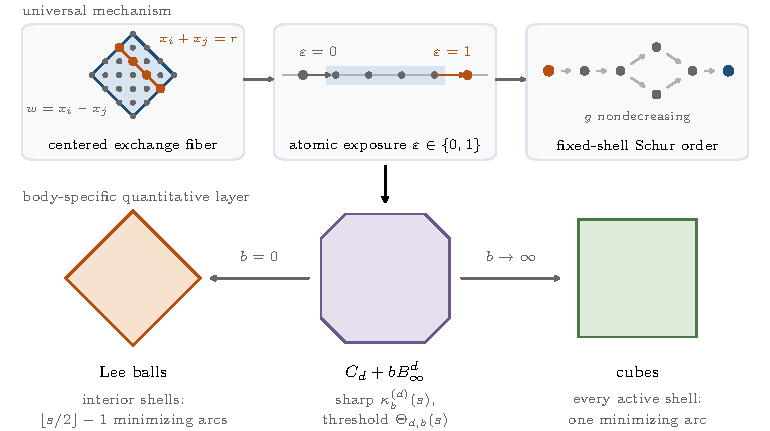
\includegraphics{fig-architecture}
  \caption{Logical architecture; the bodies are two-dimensional schematics.
  Above: a centered exchange fiber, the straight slice on which the other
  coordinates and $r=x_i+x_j$ are fixed while $w=x_i-x_j$ varies; the atomic
  exposure $\varepsilon\in\{0,1\}$ of one balancing transfer, according to
  whether the moved endpoint leaves the opposite interval; and the order
  their sum produces on a fixed shell, drawn as the majorization Hasse
  diagram of $s=6$ in $d=3$ and oriented from skewed to balanced, the
  direction along which $g$ does not decrease.  Below: the quantitative
  layer, which is body-dependent.  The structural theorem of Section~\ref{sec:structural}
  evaluates it on the interpolating family $C_d+bB_\infty^d$ and recovers
  equal Lee balls and equal cubes as the two degenerate regimes, the cases
  without factorization and without surcharge; the Lee count is that of the
  interior shells $4\le s\le2t-2$.}
  \label{fig:architecture}
\end{figure}

\subsection{Organization}

Section~\ref{sec:related} positions the result within covariogram,
majorization, and discrete-rearrangement theory.
Section~\ref{sec:universal} proves the universal exchange-fiber calculus.
Section~\ref{sec:shapes} develops the sharp Lee specialization and its radial
equality theory.  Section~\ref{sec:polytope-phases} proves the cube constant
and the two interpolation phenomena, and Section~\ref{sec:structural} the
structural evaluation and its facet threshold.
Section~\ref{sec:quotient-boundary} gives an explicit finite-quotient
reversal.  The exact lens enumerator and reproduction details are deferred to
the appendices.

\section{Related work}
\label{sec:related}

In each neighbouring literature the
overlap function, or a global rearrangement of it, is the object of study;
here the two bodies are fixed and known, and the object of study is the
order of the overlap values along the majorization graph of one $\ell_1$
shell, resolved edge by edge into exact integer increments.

\subsection{Covariograms, cross-covariograms, and translated intersections}

The function
\[
 u\mapsto J_{p,q}^{(d)}(u)
 =
 \left|
 B_1^d(p)\cap(B_1^d(q)-u)
 \right|
\]
is a discrete cross-covariogram; more generally this paper studies
$u\mapsto |(K\cap\Z^d)\cap((L\cap\Z^d)-u)|$ for two known symmetric convex
bodies $K,L$.  The continuous covariogram originated in random-set and
integral geometry, and geometric tomography made the inverse
question---which bodies are determined by all translated-overlap
volumes?---a central theme~\cite{Matheron75,Gardner06,Bianchi23Survey}.
For planar convex bodies that program developed through partial results and
the resolution of Matheron's conjecture
\cite{Bianchi05Matheron,AverkovBianchi09}, with a complementary phase
retrieval formulation~\cite{BianchiGardnerKiderlen11}, and unequal sets have
their own reconstruction problem~\cite{Bianchi09Cross}.  Translated
intersections also appear in direct geometric inequalities: the radial
dependence of the continuous intersection volume is tied to
ellipsoids~\cite{MeyerReisnerSchmuck93}, and recent unpublished work of
Bianchi, Burchard, and Lin (arXiv:2508.03887) studies strict concavity of
cross-covariograms along Euclidean segments.

For finite lattice sets, discrete covariograms were developed in connection
with sums, projections, sections, and reconstruction
\cite{GGZ05,AverkovLangfeld12}; homometric lattice-convex sets show that the
complete discrete covariogram can have nontrivial equality classes
\cite{RosenblattSeymour82,AverkovLangfeld16}.  Alonso-Guti\'errez, Lucas
Mar\'in, and Mart\'in Go\~ni studied the lattice-point-enumerator
covariogram $\widetilde g_K(x)=\mathrm G_n\bigl(K\cap(x+K)\bigr)$ and the
associated covariogram ball bodies in connection with discrete projection
inequalities of Zhang type~\cite{AlonsoLucasMartinGoni25}; their results
concern radial integrals and inclusions between ball bodies.  Discrete
tomography reconstructs finite sets from X-rays, with a corresponding notion
of stability under noisy or inconsistent projection data
\cite{GardnerGritzmann97,AlpersGritzmann06}.  Our equality classes are not
homometric pairs and our stability is not robustness to perturbed data;
both are intrinsic to the values of one fixed cross-covariogram along the
integer unit-transfer graph.

\subsection{Lee geometry, compositions, and lattice tilings}

Lee introduced the nonbinary metric~\cite{Lee58} and its channel-theoretic
form followed soon afterwards~\cite{ChiangWolf71}.  In finite Lee spaces the
natural association relations are indexed by Lee compositions rather than by
scalar Lee distance alone, a distinction underlying the Lee scheme and its
linear-programming theory \cite{Astola82Scheme,AstolaTabus16}: composition
sensitivity is itself classical.  Our refinement fixes the total Lee length
of a translation on $\Z^d$ and resolves the change between comparable
compositions into exact increments.  Tiling and packing by Lee balls
\cite{GolombWelch70,Post75,Horak09Tilings,HorakKim18,ZhangZhou19,LeungZhou20}
and perfect, quasi-perfect, diameter-perfect, and dense Lee codes
\cite{Etzion11,HorakAlBdaiwi12,ZhangGe24Diameter,XiaoZhou24} constrain
disjoint or near-disjoint families of translates rather than comparing the
lens deficits of two translations on one shell.
Explicit finite-$q$ intersection formulas do occur in identifying-code
bounds~\cite{RD21} and through generating functions for Lee-ball volumes
~\cite{BhattacharyaBanerjee19}, but not the fixed-shell comparison
structure studied here.

One recent preprint is a close methodological neighbour.  Albader
(arXiv:2606.17527) studies local fault repair
of perfect resource placements in dense two-dimensional Gaussian networks
and, for that repair geometry, proves exact replacement numbers together
with the sharp minimum-overlap formula $\Omega_G(t)=t+1$ for $t\ge2$ among
minimum-size repairs.  The overlap lower bound there is obtained in the
rotated coordinates $u=x+y$, $v=x-y$, in which planar Lee balls become
parity-constrained squares: exactly the
two-dimensional case of the sum--difference slicing used throughout
Section~\ref{sec:universal} and of the diamond-to-square parity treatment
opening Section~\ref{sec:shapes}, and both arguments exploit two parity
classes to obtain exact counts.  The results are nevertheless disjoint.
The optimization there is over replacement placements repairing a failed
Lee cell in the plane, and its extremal quantity is a minimum overlap among
minimum-size repairs; here the two bodies are fixed, the variable is their
relative integer translation on a prescribed $\ell_1$ shell in every
dimension $d\ge3$, and the extremal data are the sharp transfer constant
$\kappa_{d,t,s}$, the minimizing arcs, and the equality pairs of a
stability inequality.  The rotation is a shared tool, not a shared theorem.

\subsection{Rearrangement, compression, and quantitative stability}

Anderson proved monotonicity of the integral of a symmetric unimodal function
over a translated symmetric convex set~\cite{Anderson55}.  Mudholkar replaced
central symmetry by invariance under a finite measure-preserving linear group
and obtained group-majorization, including permutation and signed-permutation
cases~\cite{Mudholkar66}; Marshall and Olkin proved convolution preservation
of Schur-concavity for continuous multivariate densities
~\cite{MarshallOlkin74}.  These continuous results rule out a volume-level
sign transition between the cross-polytope and cube.

The closest qualitative antecedent on the lattice comes from DT functions.
Hollander, Proschan, and Sethuraman established their composition properties
~\cite{HollanderProschanSethuraman77} and in a companion paper proved the DT
property of \emph{overlapping sums} of independent random variables
~\cite{HollanderProschanSethuraman81}.  Theorems~4--5 of Joag-Dev and
Sethuraman formulate the composition theorem for any
coordinate-permutation-invariant Borel measure for which the composition is
well defined~\cite{JoagDevSethuraman92}; taking that measure to be
$\sum_{z\in\Z^d}\delta_z$ and the two kernels to be indicators of symmetric
convex bodies yields the nonnegative sign of every lattice balancing
transfer.  As announced in the introduction, we do not claim that sign, that
is, the inequality of Corollary~\ref{cor:general-majorization}, as new.  What
the preservation route does not produce is an increment value, an equality
criterion, or an extremal set: it returns one inequality per comparison,
whereas Theorem~\ref{thm:general-transfer} returns the identity
~\eqref{eq:general-transfer} expressing that comparison as a sum of
$\{0,1\}$-valued parity-fiber exposures over explicitly indexed lattice
fibers, and forgetting which fibers are exposed recovers the DT conclusion.
To the best of our knowledge that identity does not appear in the DT
literature.  The results below all depend on which fibers are exposed: the
fiberwise equality certificate of
Corollary~\ref{cor:general-majorization}, the closed constants of
Theorems~\ref{thm:sharp-kappa} and~\ref{thm:cube-sharp}, the extremal
classifications of Theorems~\ref{thm:arc-classification}
and~\ref{thm:pair-rigidity}, and the structural evaluation of
Section~\ref{sec:structural}.

The centered exchange-fiber property should also be compared with existing
discrete set classes.  It is a sectional condition: every two-coordinate
fiber, in sum--difference coordinates, must be a centered parity interval.
It is implied by convex hyperoctahedral lattice sections, but it is not an
exchange axiom in the sense of discrete convex analysis.  The M-convex and
jump-system exchange axioms~\cite{Murota03,BouchetCunningham95} constrain
how one point of a set can move toward another point of the \emph{same} set
and impose no symmetry, whereas the present property constrains the shape
and centering of one-dimensional parity sections and imposes no exchange
between distinct points.  Neither condition subsumes the other: the set
$\{(0,0),(2,2)\}\subset\Z^2$ has centered exchange fibers (both difference
fibers are the single point $\{0\}$) but violates the two-step exchange
axiom of a jump system, since no lattice point adjacent to $(0,0)$ toward
$(2,2)$ admits a second step into the set, and for the same reason it is
not M$^\natural$-convex; conversely, the singleton $\{(1,0)\}$ is both a
trivial M-convex set and a trivial jump system, yet its difference fiber
$\{1\}$ is not centered.  We therefore use a separate name.

Classical symmetric-decreasing rearrangement compares a function or a set
with a centered equimeasurable profile; the Riesz inequality and its
multilinear extensions are standard instances
\cite{Riesz30,BrascampLiebLuttinger74,LiebLoss01}.  The abstract vector order
used here is classical majorization, equivalently generated by elementary
balancing transforms
\cite{HardyLittlewoodPolya52,MarshallOlkinArnold11}.  Equality in
continuous Riesz rearrangement and local symmetrization by polarization have
their own theories~\cite{Burchard96,BrockSolynin00}, and monotone or
supermodular integrands provide a broader functional
setting~\cite{BurchardHajaiej06}.  Discrete convolution and Schwarz
rearrangements have been developed on graphs and integer
lattices~\cite{Hajaiej10,GuptaSteinerberger24,HajaiejHanHua22}, and
coordinate compression is a classical local-to-global method in discrete
isoperimetry~\cite{BollobasLeaderCompression91,BarberErde18}.  All of these
move the sets or functions: a rearrangement recenters them, and compression
changes a set to improve a boundary or shadow.  Recentering in particular
erases the distinction between the translations $(2,0)$ and $(1,1)$, which
is precisely the fixed-shell variable retained here.  Our local move acts on
the integer translation partition rather than on either radial profile, and
its effect is an exact finite difference.

Quantitative stability normally asks whether an analytic deficit controls
distance from an extremal orbit.  Sharp quantitative isoperimetry and its
transport developments and surveys provide prototypes
\cite{FuscoMaggiPratelli08,FigalliMaggiPratelli10,Fusco15};
stability for Riesz rearrangement gives a closer continuous correlation
analogue~\cite{CarlenMaggi17}.  Discrete lattice stability results typically
describe large near-minimizers by their proximity to structured sets such as
zonotopes~\cite{BarberErdeKeevashRoberts23}.  Our statements have a
different exact finite structure: on one fixed integer shell the metric is
the minimum number of unit Robin Hood transfers, the deficit is a sum of
explicit integer arc weights, and the extremal constants, arcs, and pairs
are evaluated and classified rather than bounded.

\subsection{Lattice-point enumeration and the finite-quotient boundary}

The normalization $B_1^d(t)=tC_d\cap\Z^d$ places Lee balls within the standard
theory of integer-point enumeration in polytopes and generating functions
\cite{BeckRobins15,Barvinok08}, and cross-polytopes have been studied through
their lattice points, intrinsic volumes, and packing density
\cite{BetkeHenk93,FejesTothFodorVigh15}.  Discrete Brunn--Minkowski
inequalities and lattice-point enumerator bounds compare counts under sums,
dilations, sections, or projections
\cite{GardnerGronchi01,IglesiasYepesZvavitch20,FreyerHenk22}, whereas our
sets and radii are fixed.  One structure from that circle of ideas does
reappear as a conclusion rather than a hypothesis: the sharp constants of
Section~\ref{sec:structural} are computed from lattice-point counts of the
same body in dimension $d-2$.  Finally, the universal theorem below uses the centered
interval cut out by a fixed coordinate-sum line together with the parity
sublattice of $\Z^d$; wrap-around destroys that slicing, and
Section~\ref{sec:quotient-boundary} shows that the naive finite-$q$
extension is false.


\section{Coordinate balancing for symmetric lattice bodies}
\label{sec:universal}

Throughout the paper the notation is divided as follows: $K,L$ denote
compact convex sets in $\R^d$ and $A,B$ finite lattice sets, typically their
lattice sections; $u,v$ are integer shift vectors and $\lambda,\mu$ their
decreasing absolute-coordinate compositions on one shell; $a,b$ are the two
entries changed by a unit transfer~\eqref{eq:intro-transfer} and $w$ is the
residual shift vector of the untouched coordinates; $p,q,t$ are radii, $s$
is a shell weight, and $K$ inside a binomial coefficient is a truncation
level, never a body.

We first isolate the part of the argument that does not depend on Lee balls.
For a finite set $A\subset\Z^d$, coordinates $i<j$, a residual vector
$z\in\Z^{d-2}$, and $r\in\Z$, define the difference fiber
\begin{equation}
 \mathcal I_A^{ij}(z,r)=
 \left\{\delta\in r+2\Z:
 x_{-\{i,j\}}=z,\
 x_i=\frac{r+\delta}{2},\
 x_j=\frac{r-\delta}{2},\ x\in A\right\}.
 \label{eq:exchange-fiber}
\end{equation}
The parity restriction is the image of $\Z^2$ under
$(x_i,x_j)\mapsto(x_i+x_j,x_i-x_j)$.

\begin{figure}[tbp]
\centering
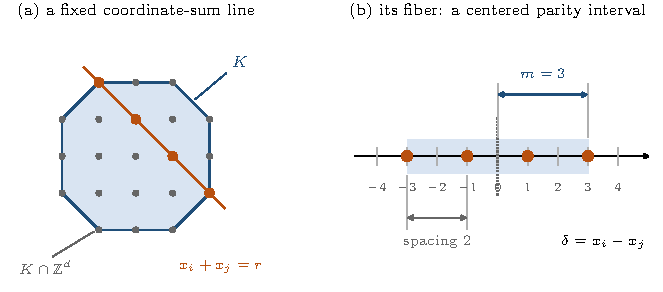
\includegraphics{fig-exchange-fiber}
\caption{The exchange fiber of Definition~\ref{def:exchange-fiber}.  On the
left, $K$ is a symmetric planar section of the body and the grey dots are the
lattice points $K\cap\Z^d$ in it.  Fixing the residual coordinates and the sum
$x_i+x_j=r$ cuts out the segment drawn in orange; its lattice points, recorded
through $\delta=x_i-x_j$, form a centered interval of one parity class.
Here the four marked points have $\delta\in\{-3,-1,1,3\}$, so $m=3$.}
\label{fig:exchange-fiber}
\end{figure}

\begin{definition}[Centered exchange fibers]
\label{def:exchange-fiber}
We say that $A$ has the \emph{centered exchange-fiber property} if every
nonempty set in~\eqref{eq:exchange-fiber} is of the form
\begin{equation}
 \{-m,-m+2,\ldots,m-2,m\}
 \qquad(m\in\Z_{\ge0},\ m\equiv r\pmod2).
 \label{eq:centered-parity-interval}
\end{equation}
No convex hull is mentioned in this definition; it is a finite, directly
checkable property of a lattice set.  Figure~\ref{fig:exchange-fiber} shows a
planar instance.
\end{definition}

For two finite sets put
\[
 g_{A,B}(u)=|A\cap(B-u)|=|\{x\in A:x+u\in B\}|.
\]

\begin{proposition}[Convex symmetric bodies have centered exchange fibers]
\label{prop:convex-exchange-fibers}
Let $K\subset\R^d$ be a compact convex set invariant under coordinate
permutations.  Then $K\cap\Z^d$ has the centered exchange-fiber property.  If
$K$ is invariant under signed coordinate permutations, then $K\cap\Z^d$ is
invariant under the same group.  Moreover, if $K$ and $L$ are both invariant
under that group, then
\[
 g_{K\cap\Z^d,L\cap\Z^d}(\gamma u)
 =g_{K\cap\Z^d,L\cap\Z^d}(u)
\]
for every signed coordinate permutation $\gamma$ and every $u\in\Z^d$.
\end{proposition}

\begin{proof}
Fix $i,j,z,r$.  Intersecting $K$ with the affine line on which the residual
coordinates and $x_i+x_j=r$ are fixed gives an interval, possibly empty or a
singleton.  The transposition $i\leftrightarrow j$ preserves this line and
maps $\delta=x_i-x_j$ to $-\delta$, so the interval is centered.  Its lattice
points have $\delta\equiv r\pmod2$ and therefore form exactly the parity
interval~\eqref{eq:centered-parity-interval}.  The last assertion follows by
applying the same signed permutation to the summation variable and to both
bodies.
\end{proof}

The atomic fact behind the general theorem is one-dimensional and exact; the
content lies in the fiberwise assembly and its quantitative
consequences.  Figure~\ref{fig:atomic-exposure} shows its
three regimes.

\begin{figure}[tbp]
\centering
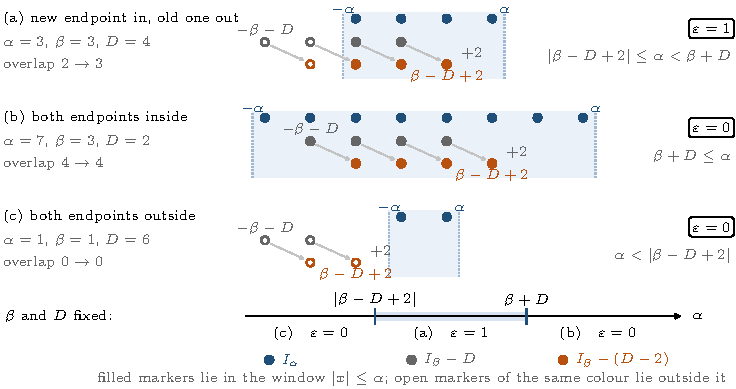
\includegraphics{fig-atomic-exposure}
\caption{The three regimes of Lemma~\ref{lem:atomic-exposure}, each drawn with
its own $(\alpha,\beta,D)$.  Translating the whole interval $I_\beta-D$ by two
deletes its left endpoint $-\beta-D$ and appends the right endpoint
$\beta-D+2$, so the overlap with $I_\alpha$ can grow by at most one point.  It
grows when the new endpoint lies in the window $|x|\le\alpha$ while the deleted
one did not~(a), and is unchanged when both lie inside~(b) or both
outside~(c); the fourth combination cannot occur because
$|\beta-D+2|\le\beta+D$.  The bottom line is the partition of the
$\alpha$-axis at fixed $\beta$ and $D$ that these three regimes
produce, which is the
criterion~\eqref{eq:atomic-exposure-criterion}.}
\label{fig:atomic-exposure}
\end{figure}

\begin{lemma}[Atomic parity-interval exposure]
\label{lem:atomic-exposure}
Let
\[
 I_\alpha=\{-\alpha,-\alpha+2,\ldots,\alpha\},\qquad
 I_\beta=\{-\beta,-\beta+2,\ldots,\beta\},
\]
where $\alpha,\beta\in\Z_{\ge0}$, and assume that
$I_\alpha$ and $I_\beta-D$ lie in the same coset of $2\Z$.  For every integer
$D\ge2$,
\begin{align}
 \varepsilon_{\alpha,\beta}(D)
 &:=
 |I_\alpha\cap(I_\beta-(D-2))|
 -|I_\alpha\cap(I_\beta-D)|                         \label{eq:atomic-exposure}\\
 &=\mathbf 1\{|\beta-D+2|\le\alpha<\beta+D\}
 \in\{0,1\}.                                        \label{eq:atomic-exposure-criterion}
\end{align}
If either interval is empty, define its exposure to be zero.
\end{lemma}

\begin{proof}
The shifted parity intervals differ only at their two endpoints:
\[
 I_\beta-(D-2)
 =\bigl((I_\beta-D)\setminus\{-\beta-D\}\bigr)
   \cup\{\beta-D+2\}.
\]
Consequently the overlap change equals
\[
 \mathbf 1\{|\beta-D+2|\le\alpha\}
 -\mathbf 1\{\beta+D\le\alpha\}.
\]
Because $|\beta-D+2|\le\beta+D$ for $\beta\ge0$ and $D\ge2$, the second
indicator can be one only when the first is one.  Their difference is the
indicator in~\eqref{eq:atomic-exposure-criterion}.  The parity-compatibility
hypothesis ensures that every endpoint displayed is in the common parity
coset.
\end{proof}

Summing this exposure over the fibers gives the transfer identity.

\begin{theorem}[Exact exchange-fiber transfer]
\label{thm:general-transfer}
Let $A,B\subset\Z^d$ be finite sets with centered exchange fibers.  Fix
coordinates $i<j$ and a shift $u\in\Z^d$, written
$u=(a,b,u_{-\{i,j\}})$ in coordinate-labelled form, whose two active entries
$a=u_i$ and $b=u_j$ are integers with $a\ge b+2$; the residual entries
$u_{-\{i,j\}}\in\Z^{d-2}$ are arbitrary.  Put
\[
 u'=u-e_i+e_j,\qquad R=a+b,\qquad D=a-b.
\]
For a nonempty fiber write $m_A^{ij}(z,r)$ for its nonnegative endpoint, and
use the analogous notation for $B$.  If a fiber is empty, put its endpoint
equal to the symbol $\varnothing$ and set
$\varepsilon_{\varnothing,\beta}
=\varepsilon_{\alpha,\varnothing}=0$.  Then
\begin{align}
 g_{A,B}(u')-g_{A,B}(u)
  =\sum_{z\in\Z^{d-2}}\sum_{r\in\Z}
  \varepsilon_{m_A^{ij}(z,r),\,
  m_B^{ij}(z+u_{-\{i,j\}},r+R)}(D),                 \label{eq:general-transfer}
\end{align}
In particular, every summand belongs to $\{0,1\}$ and the increment is
nonnegative.  The transfer is flat if and
only if every fiber fails the endpoint-exposure condition
~\eqref{eq:atomic-exposure-criterion}.
\end{theorem}

\begin{proof}
Fix $z$ and write $r=x_i+x_j$, $\delta=x_i-x_j$.  The first membership
condition is
$\delta\in\mathcal I_A^{ij}(z,r)$.  For $x+u\in B$, the translated coordinate
sum and difference are $r+R$ and $\delta+D$, so the second condition is
\[
 \delta+D\in
 \mathcal I_B^{ij}(z+u_{-\{i,j\}},r+R).
\]
Thus this slice contributes the overlap of two centered parity intervals, the
second translated by $-D$.  Their parity cosets agree because
$R-D=2b$.  The transfer fixes $R$ and replaces $D$ by $D-2$.
Lemma~\ref{lem:atomic-exposure} gives the displayed exposure for this slice;
summing the disjoint slices proves~\eqref{eq:general-transfer}.  Since all
summands are nonnegative, their sum vanishes exactly when each one does.
\end{proof}

For nonnegative integer vectors of equal coordinate sum, write $x\succeq y$
when
\[
 \sum_{k=1}^h x_k^\downarrow
 \ge\sum_{k=1}^h y_k^\downarrow\qquad(1\le h<d).
\]

\begin{corollary}[Symmetric lattice cross-covariogram majorization]
\label{cor:general-majorization}
Let $K,L\subset\R^d$ be compact convex sets invariant under signed coordinate
permutations, and put $A=K\cap\Z^d$, $B=L\cap\Z^d$.  If
integer shifts $u,v\in\Z^d$ satisfy
\begin{equation}
 |u|^\downarrow\succeq |v|^\downarrow,
 \qquad \|u\|_1=\|v\|_1,
 \label{eq:general-majorization}
\end{equation}
then
\begin{equation}
 g_{A,B}(u)\le g_{A,B}(v).                           \label{eq:general-schur}
\end{equation}
The same conclusion holds for any signed-permutation-invariant finite sets
$A,B$ with centered exchange fibers.  For comparable $u,v$, equality holds
if and only if all exposures vanish on one---equivalently, on every---monotone
unit-transfer chain from $|u|^\downarrow$ to $|v|^\downarrow$.
\end{corollary}

\begin{proof}
Signed-permutation invariance reduces to nonnegative decreasing shifts;
Theorem~\ref{thm:general-transfer} itself imposes no sign condition on the
entries.  Integer majorization is generated by unit Robin Hood transfers
followed by permutations~\cite{MarshallOlkinArnold11}; see also
Lemma~\ref{lem:transfer-distance} for a self-contained construction.  Apply
Theorem~\ref{thm:general-transfer} along such a chain.  The endpoint
difference is a sum of nonnegative arc weights, so it is zero exactly when
every arc on the chain has zero weight.  The reason one chain suffices is
that the endpoint difference $g_{A,B}(v)-g_{A,B}(u)$ does not depend on the
chain: if the arc weights of one monotone chain sum to zero, the same number
is the sum of the nonnegative arc weights of any other monotone chain, whose
arcs must therefore all be flat as well.
\end{proof}

Throughout the paper we distinguish three levels of equality language.
\emph{Local edge equality} means that one unit-transfer arc has weight zero;
Theorem~\ref{thm:general-transfer} characterizes it fiberwise.
\emph{Comparable endpoint equality} means $g_{A,B}(u)=g_{A,B}(v)$ for a
comparable pair~\eqref{eq:general-majorization}; by
Corollary~\ref{cor:general-majorization} it is equivalent to local edge
equality along one---equivalently every---monotone chain.
\emph{Extremizer uniqueness} asks whether the minimizing composition of a
shell is unique modulo signed permutations.  All three levels are relative
to the majorization order: strict Schur-concavity is an order-theoretic
statement about comparable pairs, and incomparable shell compositions may
take equal overlap values (Remark~\ref{rem:incomparable}).  For a general
body, the fiberwise conditions above are a \emph{certificate}: a prescribed
transfer or chain can be tested fiber by fiber, but no geometric
description of the flat transfers is asserted.  The \emph{geometric
classifications} of extremal arcs and pairs proved in this paper are
body-specific results: Theorems~\ref{thm:arc-classification}
and~\ref{thm:pair-rigidity} for Lee balls and
Corollary~\ref{cor:cube-arc-classification} for cubes.

\begin{remark}[Relation to DT composition]
\label{rem:dt-antecedent}
The weak nonnegative sign in Corollary~\ref{cor:general-majorization} can
alternatively be recovered from the classical DT preservation framework of
Hollander, Proschan, and Sethuraman, in the formulation of Joag-Dev and
Sethuraman~\cite{HollanderProschanSethuraman77,HollanderProschanSethuraman81,
JoagDevSethuraman92}.  We do not use that route in any proof below:
Theorem~\ref{thm:general-transfer} resolves the increment into integer
endpoint exposures and thereby supplies the strictness, equality, and
sharp-stability information that the preservation framework does not record.
\end{remark}

The set theorem also has a functional form.  It is useful when the profiles
are not indicators of one body.

\begin{corollary}[Exchange-fiber profile correlations]
\label{cor:general-profiles}
Let $f,g:\Z^d\to\R_{\ge0}$ be finitely supported and invariant under signed
coordinate permutations.  Suppose every positive superlevel set of $f$ and
of $g$ has centered exchange fibers.  Then
\[
 u\longmapsto\sum_{x\in\Z^d}f(x)g(x+u)
\]
is Schur-concave in $|u|^\downarrow$ on each fixed $\ell_1$ shell.
In particular, this applies when the superlevel sets are lattice sections of
hyperoctahedrally invariant compact convex sets.
\end{corollary}

\begin{proof}
Use the layer-cake identities
$f(x)=\int_0^\infty\mathbf1_{\{f(x)>s\}}\,ds$ and similarly for $g$.
Tonelli's theorem expresses the correlation as a nonnegative double integral
of cross-covariograms of superlevel sets.  Apply
Corollary~\ref{cor:general-majorization} pointwise in the two levels.
\end{proof}

The centered exchange-fiber condition is sufficient, not asserted to be
necessary.  The following examples show that neither ingredient in the convex
hyperoctahedral hypothesis can be dropped wholesale.

\begin{example}[Sharpness examples for the hypotheses]
\label{ex:general-sharpness}
In dimension two, let
\[
 X=\{0,\ \pm e_1,\ \pm e_2,\ \pm2e_1,\ \pm2e_2\}.
\]
This finite set is unconditional and permutation invariant, but its diagonal
fiber at $r=2$ has a hole.  Direct counting gives
\[
 g_{X,X}(2,0)=3>2=g_{X,X}(1,1),
\]
so balancing has increment $-1$.  Filling the diagonal holes to obtain
$B_1^2(2)$ changes the same increment to $8-5=3$.

Conversely, convexity without coordinate-permutation symmetry is insufficient.
For the lattice rectangle
$Y=([-5,5]\times[-1,1])\cap\Z^2$,
\[
 g_{Y,Y}(2,0)=9\cdot3=27>20=10\cdot2=g_{Y,Y}(1,1).
\]
These counterexamples show that a sign reversal becomes possible outside the
sufficient class above; they do not claim that every set outside that class
must reverse.
\end{example}

On any finite shell on which all unit-transfer arcs are strict, their least
integer weight is automatically a sharp slope against shortest
unit-transfer distance for comparable pairs.  Determining that least weight
is not universal: it is the body-specific third layer developed next.


\section{Lee-ball calculus and sharp stability}
\label{sec:shapes}

For $d\ge1$ and $t\in\Z_{\ge0}$, let
\[
 C_d=\{x\in\R^d:\|x\|_1\le1\},\qquad
 B_1^d(t)=tC_d\cap\Z^d.
\]
Its lattice count is
\begin{equation}
 L_d(t)=|B_1^d(t)|
 =\sum_{j=0}^{\min(d,t)}2^j\binom dj\binom tj.
 \label{eq:crosscount}
\end{equation}
An exact all-scale rational enumerator for the equal-radius lens---a
closed bivariate generating function together with a binomial extraction
formula---is stated and proved as Theorem~\ref{thm:crossgf} in
Appendix~\ref{app:crossgf-proof}.  It is not needed for the balancing
calculus and reappears only once, as an alternative derivation of one
atomic identity in the proof of Theorem~\ref{thm:sharp-kappa}.  One of its
special cases is worth recording here:
\[
 |B_1^2(2)\cap(B_1^2(2)-2e_1)|=5
 \qquad\text{whereas}\qquad
 |B_1^2(2)\cap(B_1^2(2)-e_1-e_2)|=8,
\]
so two shifts of the same Lee weight can have different lattice lenses, and
scalar Lee distance does not determine the overlap.

\subsection{Exact balancing calculus}

Recall that for $\lambda,\mu\in\Z_{\ge0}^d$ with equal coordinate sum, we
write $\lambda\succeq\mu$ when their decreasing rearrangements satisfy
\[
 \sum_{i=1}^k \lambda_i^\downarrow\ge
 \sum_{i=1}^k \mu_i^\downarrow\qquad(1\le k<d).
\]
Thus $\lambda\succeq\mu$ means that $\lambda$ is at least as
coordinate-concentrated as $\mu$.  For radii $p,q\in\Z_{\ge0}$, define the unequal-radius Lee lens
\[
 J_{p,q}^{(d)}(u)=\left|\left\{x\in\Z^d:
 \|x\|_1\le p,\ \|x+u\|_1\le q\right\}\right|.
\]
Figure~\ref{fig:transfer} shows the elementary move underlying the
order: one unit passes from the larger coordinate to the smaller coordinate
while their sum remains fixed.

\begin{figure}[htbp]
\centering
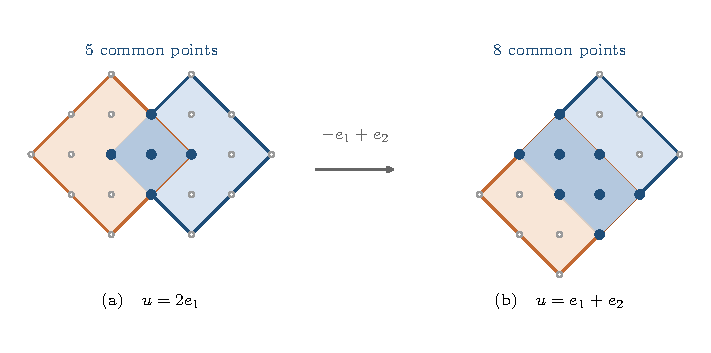
\includegraphics{fig-transfer}
\caption{A unit balancing transfer in translation-composition space.  The
shifts $u=(3,1)$ and $u'=(2,2)$ lie on the same shell $u_1+u_2=4$, and the
move sends one unit from the larger coordinate to the smaller one.}
\label{fig:transfer}
\end{figure}

For $p,q\in\Z_{\ge0}$, $c\in\Z$, and $\epsilon\in\{0,1\}$, let
\begin{equation}
 n_\epsilon(p,q;c)=
 \left|[-p,p]\cap[-c-q,-c+q]\cap(2\Z+\epsilon)\right|.  \label{eq:parity-count}
\end{equation}
Extend $n_\epsilon(p,q;c)$ by zero whenever $p<0$ or $q<0$.  For nonnegative
radii these are elementary interval counts.  If
$\ell=\max\{-p,-c-q\}$ and $h=\min\{p,-c+q\}$, let
$\rho_\epsilon(\ell)\in\{0,1\}$ be the residue satisfying
$\rho_\epsilon(\ell)\equiv\epsilon-\ell\pmod2$.  The first integer of parity
$\epsilon$ at or above $\ell$ is $\ell+\rho_\epsilon(\ell)$, and hence
\begin{equation}
 n_\epsilon(p,q;c)=
 \max\left\{0,1+\left\lfloor
 \frac{h-\ell-\rho_\epsilon(\ell)}2\right\rfloor\right\}. \label{eq:parity-floor}
\end{equation}
Thus the parameter space is cut by finitely many affine endpoint and parity
walls.  The next theorem evaluates the increment of a balancing step.

\begin{theorem}[Exact two-coordinate balancing calculus]
\label{thm:transfer-calculus}
For $p,q,a,b\in\Z_{\ge0}$ with $a\ge b+2$, put
\[
 M_{p,q}(a,b)=\left|\left\{(x,y)\in\Z^2:
 |x|+|y|\le p,\ |x+a|+|y+b|\le q\right\}\right|.
\]
Write $R=a+b$ and $D=a-b$.  Then
\begin{align}
 M_{p,q}(a-1,b+1)-M_{p,q}(a,b)
 &=\Phi_{p,q}(R,D)                                      \label{eq:transfer-kernel}\\
 &:=\sum_{\epsilon=0}^1 n_\epsilon(p,q;R)
 \bigl(n_\epsilon(p,q;D-2)-n_\epsilon(p,q;D)\bigr).    \label{eq:transfer-parity-sum}
\end{align}
Each bracket in~\eqref{eq:transfer-parity-sum} belongs to $\{0,1\}$.  In
particular $\Phi_{p,q}(R,D)\ge0$, and equality holds if and only if
\begin{equation}
 n_\epsilon(p,q;R)
 \bigl(n_\epsilon(p,q;D-2)-n_\epsilon(p,q;D)\bigr)=0
 \quad(\epsilon=0,1).                                  \label{eq:local-equality}
\end{equation}
For radii that differ by at most one, the chamber formula collapses to
\begin{equation}
 \Phi_{p,q}(R,D)=
 \begin{cases}
  \frac12(p+q-R+1)_+,& |p-q|=1\ \text{and }D=2,\\[2pt]
  (p+q-R+1)_+,&\text{otherwise},
 \end{cases}
 \qquad (|p-q|\le1).                                  \label{eq:near-equal-transfer-linear}
\end{equation}
In particular,
$\Phi_{t,t}(R,D)=(2t-R+1)_+$, so every equal-radius balancing move is
strict exactly when $a+b\le2t$.
\end{theorem}

\begin{proof}
Use the parity-preserving diamond-to-square coordinates
\[
 r=x+y,\qquad w=x-y.
\]
They biject $\Z^2$ with
$\Lambda=\{(r,w)\in\Z^2:r\equiv w\pmod2\}$, and
\[
 |x|+|y|=\max\{|r|,|w|\}.
\]
The radius-two example in Fig.~\ref{fig:square-map} displays the bijection
and the two interlaced parity classes directly.

\begin{figure}[htbp]
\centering
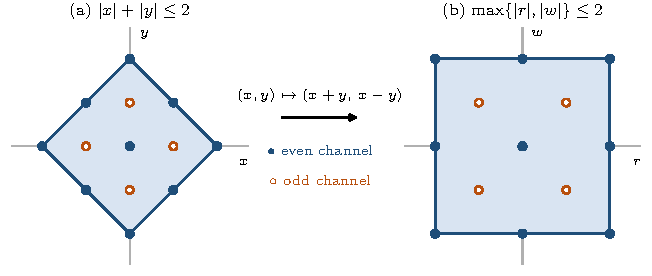
\includegraphics{fig-square-map}
\caption{The diamond-to-square map.  The transformation
$T(x,y)=(x+y,x-y)$ sends the integer points of $B_1^2(2)$ to the points of
$[-2,2]^2$ lying in
$\Lambda=\{(r,w)\in\mathbb Z^2:r\equiv w\pmod2\}$.  Filled and open circles
distinguish the even--even and odd--odd channels, which the map keeps
separate.}
\label{fig:square-map}
\end{figure}

Writing $R=a+b$ and $D=a-b$, the second norm is
\[
 \max\{|r+R|,|w+D|\}.
\]
Consequently the points being counted are
\begin{equation}
 \bigl(I(R)\times I(D)\bigr)\cap\Lambda,\qquad
 I(c)=[-p,p]\cap[-c-q,-c+q]\cap\Z.       \label{eq:parity-rectangle}
\end{equation}
The balancing step fixes $R$ and replaces $D\ge2$ by $D-2$.  Splitting
$\Lambda$ into its even--even and odd--odd classes gives
\[
 M_{p,q}(a,b)=\sum_{\epsilon=0}^1
 n_\epsilon(p,q;R)n_\epsilon(p,q;D),
\]
and subtraction proves the parity expansion~\eqref{eq:transfer-parity-sum},
hence~\eqref{eq:transfer-kernel}.

It remains to identify the sign without imposing any relation between $p$
and $q$, and this is exactly the atomic exposure of
Lemma~\ref{lem:atomic-exposure}.  Fix a parity class $\epsilon$.  The
section $[-p,p]\cap(2\Z+\epsilon)$ is a centered parity interval: it equals
$I_\alpha$ with
\[
 \alpha=\max\{n\in\Z_{\ge0}:n\le p,\ n\equiv\epsilon\pmod2\},
\]
and it is empty exactly when no such $n$ exists.  Likewise,
$z\in[-c-q,-c+q]\cap(2\Z+\epsilon)$ if and only if
$z+c\in[-q,q]\cap(2\Z+\epsilon+c)$, so with
\[
 \beta=\max\{n\in\Z_{\ge0}:n\le q,\ n\equiv\epsilon+c\pmod2\}
\]
one has $[-c-q,-c+q]\cap(2\Z+\epsilon)=I_\beta-c$, again with the empty
convention.  Hence
\[
 n_\epsilon(p,q;c)=|I_\alpha\cap(I_\beta-c)|.
\]
Figure~\ref{fig:parity-rectangle} shows a chamber in which one parity channel
gains a point while the other exchanges one point without changing its
count.

\begin{figure}[htbp]
\centering
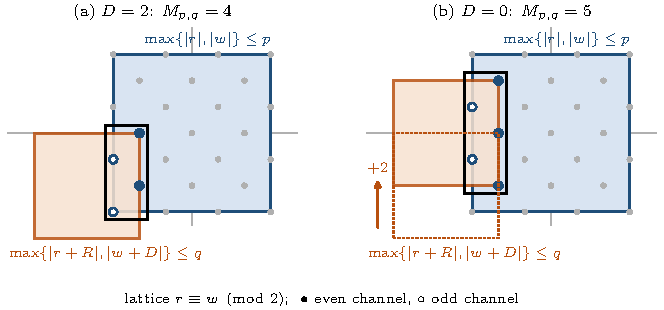
\includegraphics{fig-parity-rectangle}
\caption{The balancing step in square coordinates for $p=3$, $q=2$, and
$(3,1)\mapsto(2,2)$, so $R=4$ and $D$ drops from $2$ to $0$.  Both bodies
become axis-parallel squares, the counted set is the rectangle
$I(R)\times I(D)$ intersected with $\Lambda$, and the move translates the
second square by two in $w$.  Here
$I(4)=\{-3,-2\}$ is fixed while the moving interval changes from
$I(2)=\{-3,-2,-1,0\}$ to $I(0)=\{-2,-1,0,1,2\}$; the channel counts pass
from $(2,2)$ to $(3,2)$, so the odd channel loses one point and gains
another and the picture asserts no set containment.}
\label{fig:parity-rectangle}
\end{figure}

Now specialize to $c=D$ and $c=D-2$.  Since $D\equiv D-2\pmod2$, the same
$\beta$ serves both displacements, and $I_\beta-D$ lies in the coset
$2\Z+\epsilon$ of $I_\alpha$.  Lemma~\ref{lem:atomic-exposure}, together
with its zero convention for empty intervals, therefore gives directly
\[
 n_\epsilon(p,q;D-2)-n_\epsilon(p,q;D)
 =\varepsilon_{\alpha,\beta}(D)\in\{0,1\}.
\]
Since both factors in~\eqref{eq:transfer-parity-sum} are nonnegative, this also
proves~\eqref{eq:local-equality}.

If $|p-q|\le1$ and $c\ge1$, then
$I(c)=[-p,q-c]\cap\Z$ whenever this interval is nonempty.  Except when
$|p-q|=1$ and $D=2$, passing from $D$ to $D-2$ adds one point in each parity
class, so the total contribution is $|I(R)|=(p+q-R+1)_+$.  In the exceptional
case $R$ is even.  Whenever $I(R)$ is nonempty, its length
$p+q-R+1$ is even, it contains equally many points of each parity, and a
direct comparison of $I(2)$ with $I(0)$ shows that exactly one parity bracket
is one.  The contribution is therefore half that length.  If $R>p+q$, then
$I(R)$ is empty in every case.  This proves
 ~\eqref{eq:near-equal-transfer-linear} and its equal-radius specialization.
\end{proof}

In every subsequent residual formula, we extend
$\Phi_{p,q}(R,D)$ by zero whenever $p<0$ or $q<0$.

\subsubsection{Boundary gaps}
Theorem~\ref{thm:transfer-calculus} intentionally assumes $D=a-b\ge2$,
which is exactly the domain of a nontrivial integer Robin Hood transfer.  If
$D=0$, there is no ordered donor coordinate.  If $D=1$, the putative move
maps $(a,b)$ to $(b,a)$ and therefore remains in the same permutation orbit,
so its lens gap is zero.  Neither case is an edge of the strict majorization
graph.  Empty chambers require no extra convention, including those that can
arise at boundary choices such as $p=0$ or $q=0$: whenever the clipped
interval is empty, the maximum with zero in~\eqref{eq:parity-floor} makes the
corresponding parity count vanish.  Thus the theorem covers all unequal
radii on its full transfer domain.  The same uniform conventions seal every
small-parameter case appearing later: for $d=2$ the closed formulas never
invoke $L_{d-3}$, because the two-dimensional line of
~\eqref{eq:kappa-closed} is stated separately; for $d=3$ and $s=3$ the
convention $L_0(r)=1$ applies; for $t=1$ the only active Lee shell is
$s=2$; the cube formulas of Theorem~\ref{thm:cube-sharp} extend through
$s=2t+1$ with vanishing factors allowed; the mixed family of
Theorem~\ref{thm:mixed-sharp} includes $b=1$ with its one extra minimizing
arc; and empty parity sections always fall under the empty-interval
convention of Lemma~\ref{lem:atomic-exposure}.  No boundary case is
omitted.  Figures~\ref{fig:transfer}--
\ref{fig:parity-rectangle} separate the three levels of the mechanism: shell
motion, the square-coordinate bijection, and the parity-resolved chamber.

The two-dimensional law lifts without loss.  For an untouched shift
$w\in\Z^{d-2}$ define its residual histogram
\begin{equation}
 h_w(r,s)=|\{y\in\Z^{d-2}:\|y\|_1=r,\ \|y+w\|_1=s\}|. \label{eq:residual-histogram}
\end{equation}

\begin{proposition}[Residual-convolution differential law]
\label{prop:residual-convolution}
Suppose $p,q\in\Z_{\ge0}$ and
$u=(a,b,w)\in\Z_{\ge0}^2\times\Z^{d-2}$ with $a\ge b+2$, and let
$u'=(a-1,b+1,w)$.  Then
\begin{equation}
 J_{p,q}^{(d)}(u')-J_{p,q}^{(d)}(u)
 =\sum_{r,s\ge0}h_w(r,s)\Phi_{p-r,q-s}(a+b,a-b),       \label{eq:lifted-kernel}
\end{equation}
where the zero-extension convention for a negative residual radius applies.
Hence the increment is
nonnegative.  It is zero if and only if every summand with $h_w(r,s)>0$ has
both parity channels in~\eqref{eq:local-equality} equal to zero.
\end{proposition}

\begin{proof}
Fix the untouched vector $y$.  Its two norms consume $r=\|y\|_1$ and
$s=\|y+w\|_1$, leaving the two-coordinate radii $p-r$ and $q-s$.
Theorem~\ref{thm:transfer-calculus} gives the increment on that slice.
Grouping slices with the same $(r,s)$ proves~\eqref{eq:lifted-kernel}.
Every term is nonnegative, so the asserted equality criterion is exact.
\end{proof}

\begin{lemma}[Balanced residual slice]
\label{lem:balanced-slice}
Let $t\in\Z_{\ge1}$, let $u=(a,b,w)\in\Z^d$ with
$a\ge b+2\ge2$, and put $u'=(a-1,b+1,w)$.  If
\[
 a+b+\|w\|_1\le2t,
\]
then there is a residual slice $y\in\Z^{d-2}$ whose two remaining radii
\[
 p'=t-\|y\|_1,\qquad q'=t-\|y+w\|_1
\]
are nonnegative, satisfy $|p'-q'|\le1$ and
$p'+q'\ge a+b$, and have
\[
 \Phi_{p',q'}(a+b,a-b)>0.
\]
Consequently
$J_{t,t}^{(d)}(u')>J_{t,t}^{(d)}(u)$.
\end{lemma}

\begin{proof}
Set $c=\|w\|_1$.  Choose integers
$0\le r_k\le|w_k|$ with
$\sum_k r_k=\lfloor c/2\rfloor$, which is possible because the capacities
$|w_k|$ sum to $c$, and put
$y_k=-\operatorname{sgn}(w_k)r_k$.  Then
\[
 \|y\|_1=\lfloor c/2\rfloor,\qquad
 \|y+w\|_1=c-\lfloor c/2\rfloor=\lceil c/2\rceil.
\]
Since $a+b\ge2$ and $a+b+c\le2t$, both residual radii are nonnegative.
They differ by at most one and satisfy
$p'+q'=2t-c\ge a+b$.  The near-equal-radius identity
~\eqref{eq:near-equal-transfer-linear} now makes the displayed local
increment positive, including its $a-b=2$ half-increment boundary.
Proposition~\ref{prop:residual-convolution} expresses the full increment as a
sum of nonnegative slice increments containing this positive term.
\end{proof}

\begin{theorem}[Lee-lens majorization and active-shell strictness]
\label{thm:cross-majorization}
Fix $d\ge2$ and $p,q\in\Z_{\ge0}$.  If $\lambda,\mu\in\Z_{\ge0}^d$ have equal coordinate sum
and $\lambda\succeq\mu$, then
\begin{equation}
 J_{p,q}^{(d)}(\lambda)\le J_{p,q}^{(d)}(\mu).     \label{eq:cross-schur}
\end{equation}
Thus every discrete cross-correlation of two Lee balls, including balls of
different radii, is Schur-concave in the decreasing rearrangement of
$(|u_1|,\ldots,|u_d|)$.
Equivalently, the joint norm enumerators are ordered in bivariate
lower-orthant order: every rectangle
$\{\|x\|_1\le p,\|x+u\|_1\le q\}$ obeys the same majorization inequality.
For equal radii $p=q=t$, if the common coordinate sum is at most $2t$, then
the inequality is strict whenever $\lambda$ and $\mu$ are not permutations
of one another.
\end{theorem}

\begin{proof}
The weak inequality is the Lee-ball specialization of
Corollary~\ref{cor:general-majorization}.  Equivalently, it follows by summing
the exact residual kernel in Proposition~\ref{prop:residual-convolution} along
a unit-transfer chain.

For equal radii in the active range, apply
Lemma~\ref{lem:balanced-slice} to the two coordinates used by each
nontrivial transfer.  It supplies one
strictly increasing slice, while Proposition~\ref{prop:residual-convolution}
makes every other slice nondecreasing.  Hence every nontrivial step, and
therefore every strict majorization chain, is strict.
\end{proof}

\subsection{Global stability and equality}
\label{sec:stability}

Let $\mathcal P_d(s)$ be the decreasing nonnegative integer partitions of
$s$ into $d$ parts.  Join $\lambda$ to $\mu$ when $\mu$ is obtained from
$\lambda$ by one unit balancing transfer followed by sorting.  Give this
directed edge the equal-radius weight
\[
 w_t(\lambda,\mu)=J_{t,t}^{(d)}(\mu)-J_{t,t}^{(d)}(\lambda).
\]
The next definition fixes, once and for all, the shell terminology used for
every body in this paper.

\begin{definition}[Active shells]
\label{def:active-shell}
Let $d\ge2$, let $A,B\subset\Z^d$ be finite signed-permutation-invariant sets whose
fixed-shell unit-transfer arc weights are all nonnegative, and let
$s\in\Z_{\ge2}$.  The shell $s$ is \emph{active} for $(A,B)$ if the least
unit-transfer arc weight
\[
 \min_{\lambda\to\mu\text{ in }\mathcal P_d(s)}
 \bigl(g_{A,B}(\mu)-g_{A,B}(\lambda)\bigr)
\]
is strictly positive, that is, if every balancing transfer on the shell
strictly increases the overlap.  A shell on which this minimum vanishes is
\emph{inactive}.
\end{definition}

Theorems~\ref{thm:sharp-kappa}, \ref{thm:cube-sharp},
\ref{thm:mixed-sharp}, and~\ref{thm:structural} make this terminology exact
for the solved families: the active shells are $2\le s\le2t$ for equal Lee
balls and $2\le s\le2t+1$ for equal cubes, while for $C_3+bB_\infty^3$ every
shell $2\le s\le2b+3$ is active and every shell $s\ge2b+4$ is inactive.

The next definition names the distinguished arc that attains the sharp
constants of the Lee and cube families.  Throughout the paper, the words
\emph{axial shift} and \emph{axial orbit} are reserved for the concentrated
shift $se_1$ and its signed-permutation orbit; the edge below is always
referred to by its full name.

\begin{definition}[Canonical axial-residual edge]
\label{def:axial-edge}
For $d\ge3$ and $s\ge2$, the \emph{canonical axial-residual edge} of
$\mathcal P_d(s)$ is the unit-transfer arc
\[
 \operatorname{sort}(s-2,2,0^{d-2})
 \longrightarrow
 \operatorname{sort}(s-2,1,1,0^{d-3}),
\]
in which the transfer acts on the pair $(2,0)$ and the residual mass $s-2$
is supported on at most one coordinate.  For $s=2$ it is the arc
$(2,0,\ldots)\to(1,1,0,\ldots)$, and for $s=3$ it is
$(2,1,0,\ldots)\to(1,1,1,0,\ldots)$.
\end{definition}

For comparable partitions $\lambda\succeq\mu$, define
\begin{equation}
 d_M(\lambda,\mu)
 =\frac12\|\lambda-\mu\|_1.                         \label{eq:maj-distance}
\end{equation}
The following self-contained lemma identifies $d_M$ with the graph distance;
it is a quantitative form of the classical fact that integer majorization is
generated by unit transfers~\cite{MarshallOlkinArnold11}.

\begin{lemma}[Exact transfer distance]
\label{lem:transfer-distance}
Let $\lambda\succeq\mu$ in $\mathcal P_d(s)$ with $\lambda\ne\mu$.  Then the
minimum number of unit balancing transfers, each followed by sorting, needed
to pass from $\lambda$ to $\mu$ equals $d_M(\lambda,\mu)$, and an optimal
chain can be chosen so that every intermediate partition majorizes $\mu$.
\end{lemma}

\begin{proof}
\emph{Lower bound.}  Let $\nu=\operatorname{sort}(\lambda-e_i+e_j)$ be one
step.  Sorting two vectors decreasingly does not increase their $\ell_1$
distance, so
$\|\nu-\lambda\|_1\le\|(\lambda-e_i+e_j)-\lambda\|_1=2$, and the triangle
inequality gives $\|\nu-\mu\|_1\ge\|\lambda-\mu\|_1-2$.  Hence each step
decreases $d_M(\cdot,\mu)$ by at most one, and at least
$d_M(\lambda,\mu)$ steps are needed.

\emph{Upper bound.}  Suppose $\lambda\ne\mu$.  Let $i$ be the first index
with $\lambda_i\ne\mu_i$; since the prefix sums of $\lambda$ dominate those
of $\mu$ and agree before $i$, necessarily $\lambda_i>\mu_i$.  Let $j>i$ be
the first later index with $\lambda_j<\mu_j$; it exists because the total
sums agree.  Then $\lambda_i\ge\mu_i+1\ge\mu_j+1\ge\lambda_j+2$, using that
$\mu$ is decreasing, so the transfer
$\nu=\operatorname{sort}(\lambda-e_i+e_j)$ is legal.

The step decreases the distance by exactly one.  Indeed, coordinate $i$ has
$|\lambda_i-1-\mu_i|=\lambda_i-\mu_i-1$ and coordinate $j$ has
$|\lambda_j+1-\mu_j|=\mu_j-\lambda_j-1$, so
$\|(\lambda-e_i+e_j)-\mu\|_1=\|\lambda-\mu\|_1-2$; sorting does not increase
the $\ell_1$ distance to the sorted $\mu$, and the lower-bound step above
prevents a decrease by more than two.

The new partition still majorizes $\mu$.  For $h<i$ and $h\ge j$ the prefix
sums of $\lambda-e_i+e_j$ are those of $\lambda$.  For $i\le h<j$ they
decrease by one, but on this range the prefix excess of $\lambda$ over $\mu$
is at least one: at $h=i$ it equals $\lambda_i-\mu_i\ge1$, and for
$i<h<j$ the choice of $j$ gives $\lambda_k\ge\mu_k$ for $i<k\le h$.  Since
sorting decreasingly only increases prefix sums, $\nu\succeq\mu$.  Iterating
$d_M(\lambda,\mu)$ times reaches $\ell_1$ distance zero, that is, $\mu$.
\end{proof}

\begin{proposition}[Shell stability bookkeeping]
\label{thm:shell-stability}
For $d\in\Z_{\ge2}$, $t\in\Z_{\ge1}$, and
$s\in\{2,\ldots,2t\}$, put
\begin{equation}
 \kappa_{d,t,s}
 =\min_{\lambda\to\mu\text{ in }\mathcal P_d(s)}
 w_t(\lambda,\mu).                                  \label{eq:kappa}
\end{equation}
Then $\kappa_{d,t,s}$ is a positive integer and, whenever
$\lambda\succeq\mu$,
\begin{equation}
 J_{t,t}^{(d)}(\mu)-J_{t,t}^{(d)}(\lambda)
 \ge \kappa_{d,t,s}d_M(\lambda,\mu)
 \ge d_M(\lambda,\mu).                              \label{eq:stability}
\end{equation}
Moreover,
\begin{equation}
 \kappa_{d,t,s}
 =\min_{\substack{\lambda\succeq\mu,\ \lambda\ne\mu\\
                   \lambda,\mu\in\mathcal P_d(s)}}
 \frac{J_{t,t}^{(d)}(\mu)-J_{t,t}^{(d)}(\lambda)}
      {d_M(\lambda,\mu)}.                            \label{eq:kappa-optimal}
\end{equation}
Hence $\kappa_{d,t,s}$ is the largest constant for which
~\eqref{eq:stability} holds simultaneously for every comparable pair on the
shell.
\end{proposition}

\begin{proof}
The graph is finite.  The strict clause of
Theorem~\ref{thm:cross-majorization} makes every edge weight positive in the
active range $s\le2t$, hence $\kappa_{d,t,s}\ge1$.  By
Lemma~\ref{lem:transfer-distance}, a shortest transfer path
from $\lambda$ to $\mu$ has $d_M(\lambda,\mu)$ edges.  Telescoping the lens
counts along it and bounding every edge by~\eqref{eq:kappa} proves
\eqref{eq:stability}.  Conversely, an edge attaining the minimum has
$d_M=1$, so no larger constant can hold for all comparable pairs.  This
proves~\eqref{eq:kappa-optimal}.
\end{proof}

\begin{namedremark}[Scope of Proposition~\ref{thm:shell-stability}]
Given positivity of the edge weights (Theorem~\ref{thm:cross-majorization})
and the identification of graph distance with $d_M$
(Lemma~\ref{lem:transfer-distance}), both~\eqref{eq:stability}
and~\eqref{eq:kappa-optimal} are formal.  What has to be done is to evaluate
$\kappa$ and its extremizers, in
Theorems~\ref{thm:sharp-kappa}, \ref{thm:arc-classification},
\ref{thm:pair-rigidity}, and~\ref{thm:structural}.
\end{namedremark}

\begin{corollary}[Complete chain equality certificate]
\label{cor:chain-equality}
Let $p,q\in\Z_{\ge0}$ and let
$\lambda=\lambda^{(0)}\to\cdots\to\lambda^{(m)}=\mu$ be any balancing chain.
Then
\[
 J_{p,q}^{(d)}(\lambda)=J_{p,q}^{(d)}(\mu)
\]
if and only if every edge of the chain satisfies the residual parity
condition of Proposition~\ref{prop:residual-convolution}.  Equivalently, all
positive residual histogram entries are supported on the two-channel zero
set~\eqref{eq:local-equality}.  In the equal-radius active range this occurs
only for $m=0$; hence a comparable pair $\lambda\succeq\mu$ has equal lens
values if and only if $\lambda=\mu$.
\end{corollary}

\begin{proof}
The endpoint difference is the sum of the nonnegative edge increments.
It vanishes exactly when each edge increment vanishes, and
Proposition~\ref{prop:residual-convolution} gives an iff criterion for each
one.  The last assertion follows from positivity in
Proposition~\ref{thm:shell-stability}.
\end{proof}

\begin{remark}[Order-theoretic scope of strictness]
\label{rem:incomparable}
The equality statements above are relative to the majorization order:
strict Schur-concavity controls comparable pairs and does not force the
lens to separate incomparable orbits.  Already on the outermost active
shell of Fig.~\ref{fig:shell-graph}, namely $\mathcal P_3(6)$ with
$t=3$, the compositions $\lambda=(4,1,1)$ and $\mu=(3,3,0)$ are
incomparable ($4>3$ but $4+1<3+3$) and are not signed permutations of one
another, yet
\[
 J^{(3)}_{3,3}(4,1,1)=4=J^{(3)}_{3,3}(3,3,0):
\]
the four lattice points in the first lens are
$(-3,0,0)$, $(-2,-1,0)$, $(-2,0,-1)$, $(-1,-1,-1)$, and in the second
$(-3,0,0)$, $(-2,-1,0)$, $(-1,-2,0)$, $(0,-3,0)$.  Coincidences of this
kind between incomparable compositions are compatible with every theorem in
this paper.
\end{remark}

\subsection{The middle-section evaluation}
\label{sec:middle-section}

The graph definition~\eqref{eq:kappa} is now evaluated by a discrete
middle-section principle.  Extend the Lee counts by the uniform conventions
\[
 L_j(r)=0\quad(r<0),\qquad
 L_0(r)=1\quad(r\in\Z_{\ge0}),\qquad
 \binom{K+e}{e}=0\quad(K<0),
\]
which cover every boundary value below.  The principle is assembled from
four short lemmas: a coordinatewise representation of the bisector layers, a
signed Erd\H{o}s--Ko--Rado incidence bound, an incidence-to-count
conversion, and an axial equality case.

\begin{namedremark}[Equality and strictness]
The proof of Theorem~\ref{thm:sharp-kappa} passes through exactly two
inequalities, recorded here once.  Fix an edge of $\mathcal P_d(s)$ with
residual shift $w\in\Z^m$, $m=d-2$, $c=\|w\|_1$, and $H=2t-s+1$; let $A_k$ be
the number of central residual points of excess $k$ and $\eta\in\{1/2,1\}$ the
kernel factor of that proof.

\emph{Link 1: noncentral slices are dropped.}  Retaining in the
residual-convolution sum of Proposition~\ref{prop:residual-convolution} only
the slices with $|r-r'|\le1$ gives
$w_t(\lambda,\mu)\ge\sum_{k\ge0}\eta A_k(H-2k)_+$, termwise since the
discarded weights are nonnegative, with equality exactly when every
noncentral slice weight vanishes.  For the canonical axial-residual edge the
kernel table $\Phi_{p,q}(2,2)$ in the proof is zero whenever $|p-q|\ge2$.

\emph{Link 2: central counts are replaced by the universal model.}
Lemmas~\ref{lem:middle-layer}--\ref{lem:central-box} give the cumulative bound
$\sum_{k\le K}\eta A_k\ge L_{m-1}(K)$ for $c>0$, and for $c=0$ every residual
point is central, with cumulative count $L_m(K)\ge L_{m-1}(K)$.  Against the
nonincreasing weights $(H-2k)_+$, Lemma~\ref{lem:cumulative-dominance} turns
this into $\sum_k\eta A_k(H-2k)_+\ge\sum_kS_{m-1}(k)(H-2k)_+$, whose closed
evaluation~\eqref{eq:kappa-closed} no longer depends on the edge.  By Abel
summation, equality holds as soon as the cumulative bound is an equality for
every $K$ with $(H-2K)_+>(H-2K-2)_+$, which
Lemma~\ref{lem:axial-equality} verifies for a concentrated residual $ce_1$
with $c\ge2$.

The minimum therefore requires equality in both links, and the canonical
axial-residual edge meets both.  All edges meeting both are determined in
Theorem~\ref{thm:arc-classification}.
\end{namedremark}

\begin{lemma}[Middle-layer representation]
\label{lem:middle-layer}
Let $m\ge1$ and $w\in\Z_{\ge0}^m$ with $c=\|w\|_1>0$; let $h$ be the number
of positive coordinates of $w$ and $z=m-h$.  For $y\in\Z^m$ put
\[
 r(y)=\|y\|_1,\qquad r'(y)=\|y+w\|_1,\qquad
 k(y)=\frac{r(y)+r'(y)-c}{2},
\]
and, for $1\le i\le h$,
\[
 q_i=\operatorname{clamp}(-y_i,0,w_i),\qquad
 \ell_i=\operatorname{dist}(-y_i,[0,w_i]),
\]
where $\operatorname{clamp}(x,0,w_i)=\min\{w_i,\max\{0,x\}\}$.  Then,
coordinatewise,
\begin{equation}
 |y_i|-|y_i+w_i|=2q_i-w_i,\qquad
 |y_i|+|y_i+w_i|=w_i+2\ell_i.             \label{eq:box-clamp}
\end{equation}
Consequently $r(y)=r'(y)$ if and only if $\sum_iq_i=c/2$ ($c$ even), and
$|r(y)-r'(y)|=1$ if and only if $\sum_iq_i\in\{(c-1)/2,(c+1)/2\}$ ($c$ odd);
in these cases
\[
 k(y)=\sum_{i=1}^h\ell_i+\sum_{i>h}|y_i|\in\Z_{\ge0}.
\]
Moreover, fix a point $q$ of the integer box $\prod_{i\le h}[0,w_i]$ and let
$e(q)$ be the number of its coordinates lying at an endpoint of its
interval.  The points $y$ realizing $q$ are parametrized by one independent
outward tail $\ell_i\in\Z_{\ge0}$ for each endpoint coordinate together with
the values $v\in\Z^z$ of the zero coordinates, and for each fixed $v$ the
number of tails of total length at most $K$ is $\binom{K+e(q)}{e(q)}$.
\end{lemma}

\begin{proof}
If $-y_i\in[0,w_i]$, then $|y_i|=q_i$, $|y_i+w_i|=w_i-q_i$, and
$\ell_i=0$.  If $-y_i>w_i$, then $q_i=w_i$, $\ell_i=-y_i-w_i$,
$|y_i|=w_i+\ell_i$, and $|y_i+w_i|=\ell_i$.  If $-y_i<0$, then $q_i=0$,
$\ell_i=y_i$, $|y_i|=\ell_i$, and $|y_i+w_i|=w_i+\ell_i$.  This proves
~\eqref{eq:box-clamp}.  Summing the first identity over $i\le h$ and noting
that a zero coordinate contributes $|y_i|-|y_i+w_i|=0$ shows that
$r(y)-r'(y)=2\sum_iq_i-c$, which gives both layer characterizations;
summing the second identity gives the excess formula, since a zero
coordinate contributes $2|y_i|$.  A coordinate with $0<q_i<w_i$ forces
$\ell_i=0$ and $y_i=-q_i$, while a coordinate with $q_i\in\{0,w_i\}$ admits
exactly one outward direction with a free tail length $\ell_i\in\Z_{\ge0}$.
The tails therefore form a free tuple in $\Z_{\ge0}^{e(q)}$, and the
nonnegative integer solutions of $\ell_1+\cdots+\ell_{e(q)}\le K$ number
$\binom{K+e(q)}{e(q)}$.
\end{proof}

\begin{lemma}[Face--layer incidence bound]
\label{lem:face-incidence}
Let $w_1,\ldots,w_h>0$ be integers with sum $c$.  Encode each
codimension-$j$ face of the box $\prod_i[0,w_i]$ by a signed $j$-set
$(P,N)$: the coordinates in $P$ are fixed at their upper endpoints $w_i$ and
those in $N$ at zero, with $P\cap N=\varnothing$ and $|P|+|N|=j$.  For
$0\le j\le h$ there are $2^j\binom hj$ such faces.  If $c=2a$ is even, at
least
\[
 2^j\binom{h-1}j
\]
of them meet the layer $\Lambda_a=\{q:\sum_iq_i=a\}$; see
Figure~\ref{fig:middle-section}.  If $c=2a+1$ is odd,
the number of incidences between codimension-$j$ faces and the two layers
$\Lambda_a$ and $\Lambda_{a+1}$ is at least
\[
 2^{j+1}\binom{h-1}j.
\]
\end{lemma}

\begin{proof}
Write $w(P)=\sum_{i\in P}w_i$ and $w(N)=\sum_{i\in N}w_i$.  On the face
$(P,N)$ the coordinate sum ranges over the integer interval
$[w(P),\,c-w(N)]$, and the free coordinates change it in unit steps, so the
face contains a point of the integer layer $\Lambda_a$ if and only if
$w(P)\le a\le c-w(N)$.

Let $c=2a$.  The face misses $\Lambda_a$ exactly when $w(P)>a$ or
$w(N)>a$; these events are mutually exclusive because
$w(P)+w(N)\le c=2a$.  Consider the family of misses with $w(P)>a$.  If two
of its members had disjoint plus supports, $P_1\cap P_2=\varnothing$ would
give $w(P_1)+w(P_2)\le c=2a$, contradicting $w(P_1),w(P_2)>a$.  Hence any
two members share a coordinate signed plus in both, so the family is
intersecting as a family of signed $j$-sets.  The signed
Erd\H{o}s--Ko--Rado theorem of Bollob\'as and Leader
~\cite{BollobasLeaderSigned97} bounds every intersecting family of signed
$j$-sets on $h$ coordinates by $2^{j-1}\binom{h-1}{j-1}$; the same argument
applies to the misses with $w(N)>a$ through their minus supports.
Therefore at least
\[
 2^j\binom hj-2\cdot2^{j-1}\binom{h-1}{j-1}
 =2^j\left[\binom hj-\binom{h-1}{j-1}\right]
 =2^j\binom{h-1}j
\]
faces meet the middle layer.  For $j=0$ there is nothing to subtract: the
single face is the whole box and meets the layer.

Let $c=2a+1$.  For $\Lambda_a$ the miss conditions are $w(P)\ge a+1$ or
$w(N)\ge a+2$; for $\Lambda_{a+1}$ they are $w(P)\ge a+2$ or
$w(N)\ge a+1$.  Every listed support has weight exceeding $c/2$, so two
disjoint supports would exceed $c$ in total, and each of the four
exceptional families is signed-intersecting exactly as before, hence of size
at most $2^{j-1}\binom{h-1}{j-1}$.  Among the $2\cdot2^j\binom hj$
face--layer incidences at least
\[
 2^{j+1}\binom hj
 -4\cdot2^{j-1}\binom{h-1}{j-1}
 =2^{j+1}\binom{h-1}j
\]
remain.
\end{proof}

\begin{figure}[htbp]
\centering
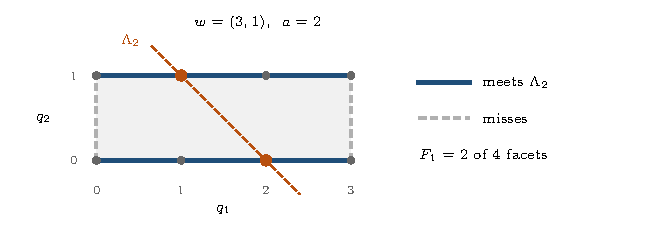
\includegraphics{fig-middle-section}
\caption{The incidence bound of Lemma~\ref{lem:face-incidence} in its
smallest nontrivial instance, $h=2$ and $w=(3,1)$, so $c=4$ and $a=2$.  A
facet is missed exactly when the coordinate it freezes is too heavy, here
the two facets $q_1=0$ and $q_1=3$; the remaining two meet $\Lambda_2$,
which matches the bound $2^1\binom{h-1}1=2$.  Neither vertex meets the
layer, again matching $2^2\binom{h-1}2=0$.}
\label{fig:middle-section}
\end{figure}

\begin{lemma}[Incidence-to-count conversion]
\label{lem:incidence-count}
In the setting of Lemma~\ref{lem:middle-layer}, fix $K\in\Z_{\ge0}$ and an
integer layer $\Lambda_a$ with $0\le a\le c$, and let $F_j(a)$ be the number
of codimension-$j$ faces of $\prod_{i\le h}[0,w_i]$ meeting $\Lambda_a$.
Then
\[
 \sum_{q\in\Lambda_a}\binom{K+e(q)}{e(q)}
 \ge\sum_{j\ge0}F_j(a)\binom Kj.
\]
Moreover, for every $j\ge0$,
\begin{equation}
 \sum_{v\in\Z^z}L_j\bigl(K-\|v\|_1\bigr)=L_{j+z}(K). \label{eq:zero-convolution}
\end{equation}
\end{lemma}

\begin{proof}
Vandermonde's identity gives
\begin{equation}
 \binom{K+e(q)}{e(q)}
 =\sum_{j=0}^{e(q)}\binom{e(q)}j\binom Kj.             \label{eq:tail-vandermonde}
\end{equation}
The binomial $\binom{e(q)}j$ is exactly the number of codimension-$j$ faces
containing $q$: such a face must fix $j$ of the $e(q)$ endpoint coordinates
of $q$, and the sign of each fixed coordinate is determined by which
endpoint that coordinate occupies.  Summing over $q\in\Lambda_a$ therefore
counts the face--point incidences of the layer.  Every face meeting the
layer contains at least one of its lattice points, so
$\sum_{q\in\Lambda_a}\binom{e(q)}j\ge F_j(a)$, and substituting into
~\eqref{eq:tail-vandermonde} proves the first claim.  For
~\eqref{eq:zero-convolution}, both sides count the set
$\{(x,v)\in\Z^j\times\Z^z:\|x\|_1+\|v\|_1\le K\}$: the left-hand side groups
its points by $v$, and the right-hand side is the Lee ball of radius $K$ in
$j+z$ coordinates.
\end{proof}

\begin{lemma}[Central Lee-bisector sections of integer boxes]
\label{lem:central-box}
Let $m\ge1$, $w\in\Z_{\ge0}^m$, and $c=\|w\|_1>0$.  For $K\in\Z_{\ge0}$, let
$N_w(K)$ count the points $y\in\Z^m$ with $k(y)\le K$ and
\[
 r(y)=r'(y)\quad(c\text{ even}),
 \qquad |r(y)-r'(y)|=1\quad(c\text{ odd}).
\]
Then
\begin{equation}
 N_w(K)\ge
 \begin{cases}
  L_{m-1}(K),&c\text{ even},\\
  2L_{m-1}(K),&c\text{ odd}.
 \end{cases}                                           \label{eq:central-box-bound}
\end{equation}
\end{lemma}

\begin{proof}
By Lemma~\ref{lem:middle-layer}, the counted points are parametrized by a
layer point $q$ (of $\Lambda_{c/2}$ when $c$ is even, of $\Lambda_{(c\pm1)/2}$
when $c$ is odd), a value $v\in\Z^z$ of the zero coordinates, and outward
tails of total length at most $K-\|v\|_1$.  Hence
\[
 N_w(K)
 =\sum_{\text{layers}}\sum_{v\in\Z^z}\sum_{q}
  \binom{(K-\|v\|_1)+e(q)}{e(q)}.
\]
For each fixed $v$ with $\|v\|_1\le K$, Lemma~\ref{lem:incidence-count}
followed by Lemma~\ref{lem:face-incidence} and the count
~\eqref{eq:crosscount} bounds the inner sum below by
$L_{h-1}(K-\|v\|_1)$ in the even case and, after adding the two layers, by
$2L_{h-1}(K-\|v\|_1)$ in the odd case.  Summing over $v$ with
~\eqref{eq:zero-convolution} gives $L_{h-1+z}(K)=L_{m-1}(K)$ and twice that
value, respectively.
\end{proof}

\begin{lemma}[Axial equality]
\label{lem:axial-equality}
If $c\ge2$ and $w=(c,0,\ldots,0)$, then equality holds in
~\eqref{eq:central-box-bound} for every $K\in\Z_{\ge0}$.
\end{lemma}

\begin{proof}
Here $h=1$ and $z=m-1$.  If $c=2a$ is even, the layer $q_1=a$ consists of
the single point $a$, which is interior to $[0,c]$ because $c\ge2$; it has
$e=0$, so no outward tail is allowed and $y_1=-a$ is forced.  If $c=2a+1$
is odd, then $c\ge3$ and the two layers $q_1\in\{a,a+1\}$ are again interior
points with $e=0$.  In either case the excess $k(y)$ reduces to the Lee norm
of the $m-1$ zero coordinates, so $N_w(K)$ equals exactly $L_{m-1}(K)$,
respectively $2L_{m-1}(K)$.
\end{proof}

The passage from cumulative section counts to weighted edge bounds uses one
further elementary lemma, stated separately because it carries the whole
majorization-of-sequences step.

\begin{lemma}[Cumulative dominance]
\label{lem:cumulative-dominance}
Let $(a_k)_{k\ge0}$ and $(b_k)_{k\ge0}$ be nonnegative sequences with
\[
 \sum_{k=0}^K a_k\ge\sum_{k=0}^K b_k
 \qquad\text{for every }K\in\Z_{\ge0},
\]
and let $(w_k)_{k\ge0}$ be nonnegative, nonincreasing, and eventually zero.
Then
\[
 \sum_{k\ge0}a_kw_k\ge\sum_{k\ge0}b_kw_k.
\]
\end{lemma}

\begin{proof}
Choose $M$ with $w_k=0$ for all $k>M$, and put $A_K=\sum_{k\le K}a_k$ and
$B_K=\sum_{k\le K}b_k$.  Abel summation gives
\[
 \sum_{k=0}^M a_kw_k=\sum_{K=0}^M A_K(w_K-w_{K+1}),
 \qquad\text{with }w_{M+1}=0,
\]
and likewise for $(b_k)$.  Every factor $w_K-w_{K+1}$ is nonnegative, so
$A_K\ge B_K$ termwise gives the claim.
\end{proof}

\begin{theorem}[Sharp active-shell constant]
\label{thm:sharp-kappa}
For $d\in\Z_{\ge2}$, $t\in\Z_{\ge1}$, and
$s\in\{2,\ldots,2t\}$, the following formulas hold.  If $d=2$, then
\begin{equation}
 \kappa_{2,t,s}=2t-s+1.                              \label{eq:kappa-d2}
\end{equation}
If $d\ge3$, put
$T_{t,s}=t-\lceil s/2\rceil$.  Then
\begin{equation}
\kappa_{d,t,s}=
\begin{cases}
L_{d-1}(t-1),&s=2,\\[2pt]
\bigl(L_{d-1}(t-1)-L_{d-3}(t-1)\bigr)/2,&s=3,\\[2pt]
L_{d-2}(T_{t,s}),&s\ge4\text{ even},\\[2pt]
L_{d-2}(T_{t,s})+L_{d-3}(T_{t,s}),
   &s\ge5\text{ odd}.
\end{cases}                                           \label{eq:kappa-closed}
\end{equation}
For $d\ge3$, the minimum on every active shell is attained by the canonical
axial-residual edge of Definition~\ref{def:axial-edge}, where $0^j$ denotes
$j$ trailing zeros:
\begin{equation}
 \operatorname{sort}(s-2,2,0^{d-2})
 \longrightarrow
 \operatorname{sort}(s-2,1,1,0^{d-3}).                \label{eq:axial-minimizer}
\end{equation}
The cases $s=2$ and $s=3$ are evaluated separately in the proof ($s=2$ has a
single arc, and for $s=3$ the two arc weights are compared exactly), while
$s\ge4$ follows from the axial-section argument.  The complete list of
minimizing arcs, on every active shell, is
Theorem~\ref{thm:arc-classification}.
Finally, extend the definition~\eqref{eq:kappa} to all $s\in\Z_{\ge2}$.  Then
\begin{equation}
 \kappa_{d,t,s}=0\qquad(s>2t),                        \label{eq:kappa-inactive}
\end{equation}
so the active shells of two equal Lee balls are exactly $2\le s\le2t$.
\end{theorem}

\begin{proof}
The two-dimensional formula follows immediately from the equal-radius clause
of Theorem~\ref{thm:transfer-calculus}, because every edge on
$\mathcal P_2(s)$ has $R=s$.

Let $d\ge3$ and consider an arbitrary edge represented before sorting by
\[
 (a,b,w)\longrightarrow(a-1,b+1,w),\qquad
 R=a+b,\qquad D=a-b\ge2.
\]
Put $m=d-2$, $c=\|w\|_1=s-R$, and $H=2t-s+1$.  On a central residual point of
excess $k$, the remaining radii $p=t-r(y)$ and $q=t-r'(y)$ differ by at most
one and satisfy
\begin{equation}
 p+q-R+1=H-2k.                                        \label{eq:central-gain}
\end{equation}
Whenever $H-2k>0$, both radii are nonnegative because $R\ge2$; otherwise the
claimed lower-bound summand is zero.  Thus
~\eqref{eq:near-equal-transfer-linear} gives the local weight
$(H-2k)_+$, except when $c$ is odd and $D=2$, when it gives half that value.
Let $A_k$ be the number of central residual points of excess $k$, and put
$\eta=1/2$ in this exceptional case and $\eta=1$ otherwise.  The two lines of
\eqref{eq:central-box-bound} imply in every case with $c>0$ that
\begin{equation}
 \sum_{k=0}^K\eta A_k\ge L_{m-1}(K).                  \label{eq:effective-central-dominance}
\end{equation}
Indeed, the factor two in the odd bound cancels the sole half-increment; when
$D>2$ the odd bound is stronger than needed.  If $c=0$, every residual point
is central and the cumulative count is $L_m(K)\ge L_{m-1}(K)$.  All
noncentral summands in Proposition~\ref{prop:residual-convolution} are
nonnegative.

Let $S_j(k)=L_j(k)-L_j(k-1)$.  Apply
Lemma~\ref{lem:cumulative-dominance} with $a_k=\eta A_k$,
$b_k=S_{m-1}(k)$, and the nonincreasing, eventually zero weight sequence
$w_k=(H-2k)_+$; the cumulative hypothesis is
~\eqref{eq:effective-central-dominance} for $c>0$ and the bound
$\sum_{k\le K}A_k=L_m(K)\ge L_{m-1}(K)$ for $c=0$.  This gives, for every
edge,
\begin{equation}
 w_t(\lambda,\mu)
 \ge \sum_{k\ge0}S_{m-1}(k)(H-2k)_+.                 \label{eq:universal-edge-lower}
\end{equation}
If $s$ is even, write $H=2T+1$ with $T=t-s/2$.  For each
$z\in\Z^{m-1}$ of norm $k\le T$, the factor $2(T-k)+1$ counts the choices of
one further integer coordinate.  Hence the right-hand side of
\eqref{eq:universal-edge-lower} is $L_m(T)$.  If $s$ is odd, write
$H=2(T+1)$ with $T=t-(s+1)/2$.  Now the factor $2(T-k)+2$ is the sum of the
same one-coordinate count and one extra choice, giving
$L_m(T)+L_{m-1}(T)$.

For $s\ge4$, the edge~\eqref{eq:axial-minimizer} has transfer pair $(2,0)$
and residual shift $(s-2,0,\ldots,0)$.  Lemma~\ref{lem:axial-equality} then
turns the central-section bound~\eqref{eq:central-box-bound} into an
equality.  Equivalently, the one-coordinate series in
Theorem~\ref{thm:crossgf} (Appendix~\ref{app:crossgf-proof}) and
lower-orthant summation give the atomic identity
\[
 \sum_{p,q\ge0}\Phi_{p,q}(2,2)X^pY^q
 =\frac{XY(1+X)(1+Y)}{(1-XY)^2}.
\]
Coefficient extraction, or direct specialization of
~\eqref{eq:transfer-parity-sum}, gives
\[
 \Phi_{p,q}(2,2)=
 \begin{cases}
  (2p-1)_+,&p=q,\\
  \min\{p,q\},&|p-q|=1,\\
  0,&|p-q|\ge2,
 \end{cases}
\]
so no noncentral residual slice adds weight.  The lower bounds above are
therefore attained, proving the last two lines of~\eqref{eq:kappa-closed}.

For $s=2$, the shell graph has the single edge
$(2,0^{d-1})\to(1,1,0^{d-2})$.  Its weight is
\[
 \sum_{y\in\Z^{d-2}}\bigl(2(t-\|y\|_1)-1\bigr)_+
 =L_{d-1}(t-1),
\]
because the linear factor counts one additional integer coordinate.
For $s=3$, put $m=d-2$ and $T=t-2$; the shell graph has exactly two edges.
Consider first $(2,1,0^{d-2})\to(1,1,1,0^{d-3})$.  Its transfer moves one
unit from the coordinate at two into a zero coordinate, so the transfer pair
is $(2,0)$ with $R=D=2$, and the residual shift is $w=e_1\in\Z^m$.  Write a
residual point as $y=(n,z)$ with $n\in\Z$ and $z\in\Z^{m-1}$; then
\[
 r=\|y\|_1=|n|+\|z\|_1,\qquad
 r'=\|y+e_1\|_1=|n+1|+\|z\|_1,
\]
so every residual slice has $|r-r'|=1$, and its remaining radii $p=t-r$ and
$q=t-r'$ differ by one.  By the displayed table, the slice weight is
$\min\{p,q\}$, which together with the zero extension for negative radii
equals $\bigl(t-\|z\|_1-\max\{|n|,|n+1|\}\bigr)_+$.  As $n$ runs over $\Z$,
the quantity $\max\{|n|,|n+1|\}$ takes every positive integer value exactly
twice, so Proposition~\ref{prop:residual-convolution} evaluates the edge
weight as
\begin{equation}
 B_T=2\sum_{z\in\Z^{m-1}}\sum_{n\ge0}
       (T+1-n-\|z\|_1)_+.                            \label{eq:s3-slice}
\end{equation}
Multiplying the three series
$\sum_{z}X^{\|z\|_1}=\bigl((1+X)/(1-X)\bigr)^{m-1}$,
$\sum_{n\ge0}X^n=1/(1-X)$, and $\sum_{T\ge0}(T+1)X^T=1/(1-X)^2$ gives
\begin{equation}
 \sum_{T\ge0}B_TX^T=
 \frac{2(1+X)^{m-1}}{(1-X)^{m+2}}
 =\frac1{2X}\left[
 \frac{(1+X)^{m+1}}{(1-X)^{m+2}}
 -\frac{(1+X)^{m-1}}{(1-X)^{m}}\right],              \label{eq:s3-generating}
\end{equation}
where the bracket identity follows from $(1+X)^2-(1-X)^2=4X$.  Since
$\sum_{r\ge0}L_j(r)X^r=(1+X)^j/(1-X)^{j+1}$ and the bracket has zero
constant term, comparing coefficients in~\eqref{eq:s3-generating} gives
\[
 B_T=\tfrac12\bigl(L_{m+1}(T+1)-L_{m-1}(T+1)\bigr)
 =\tfrac12\bigl(L_{d-1}(t-1)-L_{d-3}(t-1)\bigr).
\]

The only other edge on the shell is $(3,0^{d-1})\to(2,1,0^{d-2})$, with
transfer pair $(3,0)$, hence $R=D=3$, and zero residual shift.  Every
residual slice has $r=r'=\|y\|_1$ and equal remaining radii
$p=q=t-\|y\|_1$, so the equal-radius clause of
Theorem~\ref{thm:transfer-calculus} gives the slice weight
$\Phi_{p,p}(3,3)=(2p-2)_+$, and the edge weight is
\[
 A_T=\sum_{y\in\Z^m}\bigl(2(t-\|y\|_1)-2\bigr)_+
 =2\sum_{y\in\Z^m}(T+1-\|y\|_1)_+.
\]
The same series give
\[
 \sum_{T\ge0}A_TX^T
 =\frac{2(1+X)^m}{(1-X)^{m+2}}
 =(1+X)\sum_{T\ge0}B_TX^T.
\]
Consequently $A_T=B_T+B_{T-1}\ge B_T$, with $B_{-1}=0$, proving the
$s=3$ line; the minimum is attained by the first edge, which is the
canonical axial-residual edge of $\mathcal P_d(3)$.  For $s=2$ the single
arc computed above is the canonical axial-residual edge of
$\mathcal P_d(2)$, so the attainment claim holds on every active shell.

For $s>2t$ and $\|u\|_1=s$, any $x$ counted by $J_{t,t}^{(d)}(u)$ would give
\[
 s=\|u\|_1\le\|x\|_1+\|x+u\|_1\le2t,
\]
a contradiction.  Hence every lens value on the shell vanishes, every arc
weight is zero, and~\eqref{eq:kappa-inactive} follows, completing the proof.
\end{proof}

\begin{corollary}[Explicit sharp deficit]
\label{cor:explicit-stability}
For every comparable $\lambda\succeq\mu$ in $\mathcal P_d(s)$, the right-hand
side of~\eqref{eq:stability} remains valid with $\kappa_{d,t,s}$ replaced by
the corresponding closed expression in~\eqref{eq:kappa-d2} or
\eqref{eq:kappa-closed}, and no larger uniform coefficient is possible.  In
particular,
\[
 \kappa_{d,t,2t}=1,\qquad
 \kappa_{d,t,2t-1}=2\quad(t\ge2).
\]
\end{corollary}

Figure~\ref{fig:shell-graph} shows one complete shell graph with the
exact arc weights that Proposition~\ref{thm:shell-stability} sums and
Theorem~\ref{thm:sharp-kappa} minimizes.

\begin{figure}[ht]
\centering
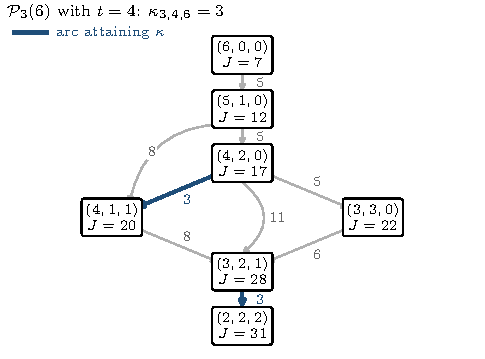
\includegraphics{fig-shell-graph}
\caption{The unit-transfer graph $\mathcal P_3(6)$ for $t=4$.  Vertices are
the partitions of six into at most three parts, labelled by their lens
values $J=J^{(3)}_{4,4}$; each arrow is one legal balancing transfer,
labelled by its exact increment.  All nine weights are positive, which
gives stability along any path, and the smallest of them is
$\kappa_{3,4,6}=3$, attained exactly on the two highlighted arcs.}
\label{fig:shell-graph}
\end{figure}
\FloatBarrier

\subsection{Classification of minimizing arcs}
\label{sec:arc-classification}

Theorem~\ref{thm:sharp-kappa} evaluates the sharp constant and exhibits one
attaining arc.  This subsection determines \emph{every} arc attaining
$\kappa_{d,t,s}$, on every active shell, and then upgrades the arc
classification to a characterization of all \emph{pairs} attaining equality
in the stability inequality~\eqref{eq:stability}.  The classification carries
a rigidity that the constant alone does not show: on all interior shells the
minimizers form one explicit family whose size depends only on
$s$---neither on the dimension nor on the radius---and no two of its members
concatenate into a distance-two extremal configuration, so equality in
~\eqref{eq:stability} is confined to single arcs.  The two outermost shells
acquire an additional, also completely described, boundary family, along
which arbitrarily long extremal geodesics do exist.  Throughout, an
arc of $\mathcal P_d(s)$ is represented modulo signed permutations by its
transfer pair $(a,b)$ with $a\ge b+2$ and its residual $w\in\Z_{\ge0}^{d-2}$,
and we keep the proof notation $m=d-2$, $R=a+b$, $D=a-b$, $c=\|w\|_1=s-R$,
and $H=2t-s+1$.  An active shell of weight $s$ is called \emph{interior}
when $d\ge3$ and $4\le s\le2t-2$, equivalently $H\ge3$; the two
\emph{outermost} shells are $s=2t-1$ ($H=2$) and $s=2t$ ($H=1$).  This is
the sense in which ``interior shell'' is used throughout the paper,
including the abstract and introduction.

\begin{definition}[Balanced-gap axial family]
\label{def:balanced-family}
For $d\ge3$ and $s\ge4$, the \emph{balanced-gap axial family} of
$\mathcal P_d(s)$ consists of the arcs
\begin{equation}
 \operatorname{sort}(c,b+2,b,0^{d-3})
 \longrightarrow
 \operatorname{sort}(c,b+1,b+1,0^{d-3}),
 \qquad 0\le b\le\tfrac{s-4}2,\quad c=s-2b-2,      \label{eq:balanced-family}
\end{equation}
that is, all unit transfers whose donor--recipient gap is exactly two and
whose residual mass $c\ge2$ is concentrated in a single coordinate.  The
member $b=0$ is the canonical axial-residual edge of
Definition~\ref{def:axial-edge}, and the family contains exactly
$\lfloor s/2\rfloor-1$ arcs.
\end{definition}

The classification proceeds by a partition of all arcs into four shapes,
displayed in Figure~\ref{fig:case-partition}.
We record the partition as a lemma so that exhaustiveness is checkable.

\begin{lemma}[Case partition]
\label{lem:case-partition}
Every arc of $\mathcal P_d(s)$, represented modulo signed permutations by
its transfer pair $(a,b)$ with $a\ge b+2$ and its residual
$w\in\Z_{\ge0}^{d-2}$, satisfies exactly one of the following, where
$D=a-b$ and $c=\|w\|_1$:
\begin{itemize}
\item[\textup{(I)}] $D=2$ and $w=ce_1$ with $c\ge2$
      \textup{(family shape)};
\item[\textup{(II)}] $c=0$, or $D=2$ and $w=e_1$
      \textup{(outer arcs)};
\item[\textup{(III)}] $w$ has at least two nonzero coordinates
      \textup{(spread residuals)};
\item[\textup{(IV)}] $D\ge3$ and $w=ce_1$ with $c\ge1$
      \textup{(wide-gap concentrated residuals)}.
\end{itemize}
\end{lemma}

\begin{proof}
After permuting residual coordinates, either $w$ has two or more nonzero
coordinates, which is Case~III and excludes the concentrated shapes of
Cases~I, II, and~IV, or $w=ce_1$ for some $c\ge0$.  In the concentrated
situation the pair $(D,c)$ with $D\ge2$ decides membership: $c=0$ lies in
Case~II only; $c=1$ lies in Case~II if $D=2$ and in Case~IV if $D\ge3$;
and $c\ge2$ lies in Case~I if $D=2$ and in Case~IV if $D\ge3$.  These
subranges of $(D,c)$ are pairwise disjoint and cover all concentrated
arcs.
\end{proof}

\begin{figure}[htbp]
\centering
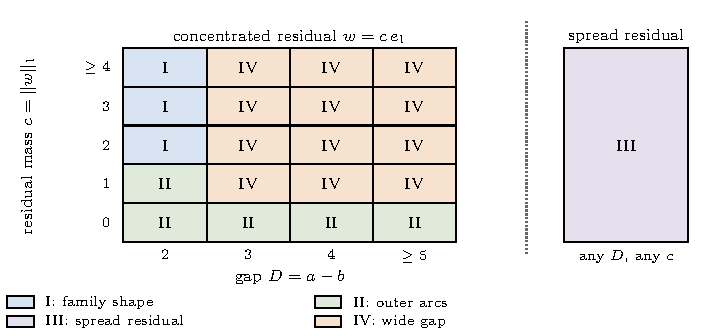
\includegraphics{fig-case-partition}
\caption{The partition of Lemma~\ref{lem:case-partition} in the invariants
$D=a-b$ and $c=\|w\|_1$.  Concentrated residuals $w=ce_1$ occupy the left
panel, where the pair $(D,c)$ alone decides the case; residuals with two or
more nonzero coordinates form Case~III regardless of $(D,c)$, shown on the
right.  Only Case~I supports the sharp family.}
\label{fig:case-partition}
\end{figure}

Four further lemmas isolate the mechanisms.  The first shows that gap-two
transfers never collect noncentral weight, whatever the residual does.

\begin{lemma}[Noncentral vanishing at gap two]
\label{lem:gap-two-vanishing}
If $|p-q|\ge2$, then $\Phi_{p,q}(R,2)=0$ for every $R\ge2$.
\end{lemma}

\begin{proof}
Recall the clipped intervals
$I(c')=[-p,p]\cap[-c'-q,-c'+q]$ from~\eqref{eq:parity-rectangle}.  If
$q\ge p+2$, then $I(0)$ and $I(2)$ both equal $[-p,p]$, so each parity
bracket in~\eqref{eq:transfer-parity-sum} vanishes.  If $p\ge q+2$, then
$I(0)=[-q,q]$ and $I(2)=[-q-2,q-2]$ both lie inside $[-p,p]$, and
$I(2)=I(0)-2$ is a parity-preserving translation, so again every parity
count is unchanged.
\end{proof}

The second lemma evaluates, exactly, the two arc shapes that will turn out
to be minimizing only near the support boundary.  Both weights are
independent of data one might expect them to depend on.

\begin{lemma}[Exact outer arc weights]
\label{lem:outer-weights}
Let $d\ge3$, $t\ge1$, $4\le s\le2t$, $m=d-2$, and $H=2t-s+1$.
\begin{enumerate}
\item[\textup{(i)}] Every arc with vanishing residual, that is, every arc
whose source and target are supported on the two transfer coordinates, has
weight
\[
 W_0=\sum_{k\ge0}S_m(k)(H-2k)_+,
\]
independently of its gap $D$.
\item[\textup{(ii)}] If $s\ge5$ is odd, the gap-two arc with residual
$w=e_1$, namely~\eqref{eq:balanced-family} with $b=(s-3)/2$ and $c=1$, has
weight
\[
 W_1=\sum_{k\ge0}L_{m-1}(k)(H-2k)_+.
\]
\item[\textup{(iii)}] Both weights satisfy
$W_0,W_1\ge\kappa_{d,t,s}$, with equality if and only if $H\le2$.
\end{enumerate}
\end{lemma}

\begin{proof}
(i) Here $w=0$, so every residual point $y$ has $r(y)=r'(y)=k$ and equal
remaining radii $p=q=t-k$.  For any $D\ge2$ the full branch of
~\eqref{eq:near-equal-transfer-linear} gives the slice weight
$(2p-R+1)_+=(H-2k)_+$, and the number of slices at norm $k$ is $S_m(k)$.

(ii) As in the $s=3$ computation inside the proof of
Theorem~\ref{thm:sharp-kappa}, write a residual point as $y=(n,z)$ with
$n\in\Z$, $z\in\Z^{m-1}$; then $|r-r'|=1$ on every slice, the half branch of
~\eqref{eq:near-equal-transfer-linear} applies, and the slice weight is
$\tfrac12(H-2j)_+$ with $j=\min\{|n|,|n+1|\}+\|z\|_1$.  Since
$\min\{|n|,|n+1|\}$ takes each value $i\ge0$ exactly twice, the number of
slices with $j$ fixed is $2\sum_{i\le j}S_{m-1}(j-i)=2L_{m-1}(j)$, and the
halves cancel the factor two.

(iii) By the evaluation of~\eqref{eq:universal-edge-lower},
$\kappa_{d,t,s}=\sum_kS_{m-1}(k)(H-2k)_+$ for $s\ge4$.  Hence
\[
 W_0-\kappa_{d,t,s}=\sum_{k\ge1}\bigl(S_m(k)-S_{m-1}(k)\bigr)(H-2k)_+,
 \qquad
 W_1-\kappa_{d,t,s}=\sum_{k\ge1}L_{m-1}(k-1)(H-2k)_+,
\]
using $L_{m-1}(k)-S_{m-1}(k)=L_{m-1}(k-1)$.  Every summand is nonnegative;
for $k\ge1$ the factors $S_m(k)-S_{m-1}(k)$ (points with nonzero last
coordinate) and $L_{m-1}(k-1)$ are strictly positive, so each difference
vanishes if and only if $(H-2k)_+=0$ for all $k\ge1$, that is, $H\le2$.
\end{proof}

\begin{lemma}[Spread residuals are strict]
\label{lem:spread-strict}
Let $d\ge4$, $4\le s\le2t$, and consider an arc whose residual $w$ has at
least two nonzero coordinates.  Then its weight strictly exceeds
$\kappa_{d,t,s}$.
\end{lemma}

\begin{proof}
Normalize signs so that $w\in\Z_{\ge0}^m$, and let
$N(j)$ count the points of the box $\prod_i[0,w_i]$ with coordinate sum
$j$; these are exactly the residual points of excess zero at the
corresponding split of $c$.  We first claim $N(j)\ge2$ for $1\le j\le c-1$.
Take any box point $r$ with coordinate sum $j$.  If there are indices
$i\ne k$ with $r_i<w_i$ and $r_k>0$, moving one unit from $k$ to $i$ gives a
second point.  Otherwise pick $i_1$ with $r_{i_1}>0$; then $r_i=w_i$ for all
$i\ne i_1$, and picking $i_2\ne i_1$ with $w_{i_2}>0$ forces, by the same
argument with the roles reversed, $r_i=w_i$ for all $i\ne i_2$ as well,
whence $r=w$ and $j=c$, a contradiction.

Now count central residual points of excess zero.  If $c$ is even, they are
the box points at coordinate sum $c/2$, so $A_0=N(c/2)\ge2$, and $\eta=1$
because the half branch requires odd $c$.  If $c$ is odd, then
$c\ge3$ because two coordinates are nonzero, and
$A_0=N\bigl((c-1)/2\bigr)+N\bigl((c+1)/2\bigr)\ge4$, while $\eta\ge1/2$.  In
all cases $\eta A_0\ge2>1=L_{m-1}(0)$.  Abel summation as in
Lemma~\ref{lem:cumulative-dominance}, with the cumulative bounds
~\eqref{eq:effective-central-dominance} at every $K$ and the strict gain
$(\eta A_0-1)\bigl(w_0-w_1\bigr)\ge\min\{H,2\}>0$ at $K=0$, shows that the
central contribution alone exceeds
$\sum_kS_{m-1}(k)(H-2k)_+=\kappa_{d,t,s}$.
\end{proof}

\begin{lemma}[Wide-gap witness]
\label{lem:wide-gap-witness}
Let $4\le s\le2t$, let the residual be concentrated, $w=ce_1$ with $c\ge2$
even, and let $D\ge3$.  Then the residual slice $y=-(c/2+1)e_1$ is
noncentral, has remaining radii $p=t-c/2-1\ge0$ and $q=t-c/2+1\le t$, and
carries
\[
 \Phi_{p,q}(R,D)=
 \begin{cases}
  H,&D\ge4,\\
  \lceil H/2\rceil,&D=3,
 \end{cases}
\]
which is strictly positive on every active shell.
\end{lemma}

\begin{proof}
The slice has $r=c/2+1$ and $r'=c/2-1$, so $|r-r'|=2$ and $q=p+2$; moreover
$R\ge D\ge3$ and $c=s-R$ even force $c\le2t-4$, hence $p\ge1$.  With
$q=p+2$, the clipped interval satisfies $I(c')=[-p,\,p+2-c']$ for every
$c'\ge2$, while $I(1)=I(0)=[-p,p]$.  Since $D\le R\le2t-c=2p+2$, the
interval $I(D)$ is nonempty, and $|I(R)|=p+q-R+1=2t-c-R+1=H$.

If $D\ge4$, then $I(D-2)$ extends $I(D)$ by the two integers
$p+3-D$ and $p+4-D$, one of each parity, so both parity brackets in
~\eqref{eq:transfer-parity-sum} equal one and
$\Phi_{p,q}(R,D)=n_0(p,q;R)+n_1(p,q;R)=|I(R)|=H$.  If $D=3$, then
$I(1)=[-p,p]$ exceeds $I(3)=[-p,p-1]$ by the single point $p$, so exactly
the bracket of parity $\epsilon\equiv p\pmod2$ equals one.  The interval
$I(R)=[-p,\,p+2-R]$ has $H$ points and its left endpoint $-p$ has parity
$\epsilon$, so $n_\epsilon(p,q;R)=\lceil H/2\rceil$.
\end{proof}

\begin{theorem}[Complete classification of minimizing arcs]
\label{thm:arc-classification}
Let $d\ge3$, $t\ge1$, $4\le s\le2t$, and $H=2t-s+1$.  Every orbit
representative $(a,b,w)$ with $a\ge b+2$ satisfies exactly one of
Cases~I--IV of Lemma~\ref{lem:case-partition}, so the following lists,
which resolve equality case by case, are exhaustive.  Modulo signed
permutations, the arcs of $\mathcal P_d(s)$ attaining $\kappa_{d,t,s}$ are
exactly the following.
\begin{enumerate}
\item[\textup{(i)}] If $H\ge3$, that is, $4\le s\le2t-2$: the balanced-gap
axial family~\eqref{eq:balanced-family}, and nothing else.  In particular
the sharp layer consists of exactly $\lfloor s/2\rfloor-1$ arcs, a number
independent of both $d$ and $t$.
\item[\textup{(ii)}] If $H=2$, that is, $s=2t-1$: the family
~\eqref{eq:balanced-family}, its continuation to $c=1$
(the arc with $b=(s-3)/2$), and every arc supported on two coordinates.
\item[\textup{(iii)}] If $H=1$, that is, $s=2t$: the family
~\eqref{eq:balanced-family} and every arc supported on two coordinates.
\end{enumerate}
For $s\in\{2,3\}$ the shell carries one, respectively two, arcs and
Theorem~\ref{thm:sharp-kappa} already lists the minimizers; for $d=2$ every
arc of $\mathcal P_2(s)$ has the same weight $2t-s+1$ by the equal-radius
clause of Theorem~\ref{thm:transfer-calculus}, so the sharp layer is the
whole shell.
\end{theorem}

\begin{proof}
Fix an arc with data $(R,D,w)$ and $c=s-R$ as above.  The proof of
Theorem~\ref{thm:sharp-kappa} bounds its weight below by
$\kappa_{d,t,s}=\sum_kS_{m-1}(k)(H-2k)_+$; by
Lemma~\ref{lem:case-partition} it suffices to decide equality in each of
Cases~I--IV.

\emph{Case I, family arcs: $D=2$, $w=ce_1$, $c\ge2$.}
Every noncentral slice has remaining radii with $|p-q|=|r-r'|\ge2$ and
contributes zero by Lemma~\ref{lem:gap-two-vanishing}.  On the central
slices, Lemma~\ref{lem:axial-equality} turns the cumulative bound
~\eqref{eq:central-box-bound} into an equality at every $K$, hence
termwise $A_k=S_{m-1}(k)$ and $\eta=1$ when $c$ is even, and
$A_k=2S_{m-1}(k)$ and $\eta=1/2$ when $c$ is odd.  Either way the weight
equals $\sum_kS_{m-1}(k)(H-2k)_+=\kappa_{d,t,s}$: every family arc is
minimizing, on every active shell.

\emph{Case II, outer arcs: $c=0$, or $(D,c)=(2,1)$.}
By Lemma~\ref{lem:outer-weights}, their weights $W_0$ and $W_1$ equal
$\kappa_{d,t,s}$ exactly when $H\le2$ and exceed it otherwise.  Note that a
gap-two arc has $c\equiv s\pmod2$, so $c=1$ occurs only on odd shells; this
is consistent with $H=2\iff s=2t-1$ odd, and no such arc exists when
$H=1$.

\emph{Case III, spread residuals.}
If $w$ has two or more nonzero coordinates (possible only for $d\ge4$),
Lemma~\ref{lem:spread-strict} gives strict inequality on every active
shell.

\emph{Case IV, concentrated residuals with wide gap: $w=ce_1$, $c\ge1$,
$D\ge3$.}
If $c$ is odd, every central slice has $|p-q|=1$, but $D\ge3$ places it in
the full branch of~\eqref{eq:near-equal-transfer-linear}, so $\eta=1$ while
~\eqref{eq:central-box-bound} bounds the cumulative counts below by
$2L_{m-1}(K)$; Lemma~\ref{lem:cumulative-dominance} then gives weight at
least $2\kappa_{d,t,s}>\kappa_{d,t,s}$.  If $c$ is even, the central
contribution equals $\kappa_{d,t,s}$ exactly as for family arcs, and
Lemma~\ref{lem:wide-gap-witness} exhibits a noncentral slice of strictly
positive weight.

By Lemma~\ref{lem:case-partition} the four verdicts cover every arc
exactly once, and they assemble into the three lists.
\end{proof}

Besides the constant, Theorem~\ref{thm:arc-classification} records the
multiplicity of the sharp layer: it is $\lfloor s/2\rfloor-1$ on every
interior shell and jumps on the two outermost shells, where the entire
two-coordinate boundary of the shell becomes sharp.  Cubes have multiplicity
one (Corollary~\ref{cor:cube-arc-classification}); the mixed family is
generically unique, with the single $b=1$ boundary exception of
Theorem~\ref{thm:mixed-sharp}.  So the degeneracy of the minimizing set is
body-dependent as well.

The stability inequality~\eqref{eq:stability} compares the lens deficit of
an arbitrary comparable pair with $\kappa_{d,t,s}$ times its transfer
distance.  Theorem~\ref{thm:arc-classification} decides equality at
distance one; the next theorem decides it at every distance and shows that
the classification of arcs already contains the complete answer.  The
content is a concatenation obstruction: two minimizing arcs never compose
into a length-two geodesic on an interior shell, so equality
in~\eqref{eq:stability} cannot propagate beyond a single transfer there,
while on the two outermost shells it propagates exactly along the
two-coordinate boundary path.  Figure~\ref{fig:rigidity} contrasts the two
behaviours.

\begin{theorem}[Rigidity of stability extremizers]
\label{thm:pair-rigidity}
Let $d\ge3$, $t\ge1$, $4\le s\le2t$, $H=2t-s+1$, and let
$\lambda\succeq\mu$ in $\mathcal P_d(s)$.  Then
\begin{equation}
 J_{t,t}^{(d)}(\mu)-J_{t,t}^{(d)}(\lambda)
 =\kappa_{d,t,s}\,d_M(\lambda,\mu)                  \label{eq:pair-equality}
\end{equation}
holds if and only if one of the following does:
\begin{enumerate}
\item[\textup{(i)}] $\lambda=\mu$;
\item[\textup{(ii)}] $d_M(\lambda,\mu)=1$ and $\lambda\to\mu$ is a
minimizing arc of Theorem~\ref{thm:arc-classification};
\item[\textup{(iii)}] $H\le2$ and both partitions are supported on two
coordinates: $\lambda=(a_1,s-a_1,0^{d-2})$ and
$\mu=(a_2,s-a_2,0^{d-2})$ with $s\ge a_1\ge a_2\ge\lceil s/2\rceil$.
\end{enumerate}
In particular, on every interior shell, that is for $H\ge3$, every
comparable pair with $d_M(\lambda,\mu)\ge2$ obeys the strict integer gap
\begin{equation}
 J_{t,t}^{(d)}(\mu)-J_{t,t}^{(d)}(\lambda)
 \ \ge\ \kappa_{d,t,s}\,d_M(\lambda,\mu)+1.        \label{eq:rigidity-gap}
\end{equation}
\end{theorem}

\begin{proof}
\emph{Sufficiency.}  Case~(i) is trivial and case~(ii) is the definition of
attainment.  For case~(iii), put $L=a_1-a_2=d_M(\lambda,\mu)$ and join the
pair by the two-coordinate path
$\nu_i=(a_1-i,\,s-a_1+i,\,0^{d-2})$, $0\le i\le L$.  Each step is legal:
its donor $a_1-i\ge a_2+1\ge\lceil s/2\rceil+1$ exceeds its recipient
$s-a_1+i$ by at least two.  Each step is an arc with vanishing residual, so
by Lemma~\ref{lem:outer-weights} its weight is $W_0=\kappa_{d,t,s}$
because $H\le2$.  Telescoping the lens counts along the path
gives~\eqref{eq:pair-equality}.

\emph{Necessity.}  Assume~\eqref{eq:pair-equality} with
$L=d_M(\lambda,\mu)\ge1$; the case $L=0$ is (i).  By
Lemma~\ref{lem:transfer-distance} choose a chain
$\lambda=\nu_0\to\nu_1\to\cdots\to\nu_L=\mu$ of exactly $L$ arcs.
Telescoping, the deficit is the sum of the $L$ arc weights, each at least
$\kappa_{d,t,s}$; equality with $\kappa_{d,t,s}L$ forces every arc of the
chain to be minimizing, and $L=1$ is case~(ii).  Let $L\ge2$.  Since
$d_M$ is one half of an $\ell_1$ metric and consecutive chain steps have
$d_M=1$, the triangle inequality forces $d_M(\nu_i,\nu_{i+2})=2$ for every
$i$: a shorter value would splice into a chain from $\lambda$ to $\mu$ of
fewer than $L$ steps, contradicting Lemma~\ref{lem:transfer-distance}.

We claim that a pair of minimizing arcs $\nu\to\nu'\to\nu''$ with
$d_M(\nu,\nu'')=2$ forces $H\le2$ with all three partitions supported on
two coordinates.  By Theorem~\ref{thm:arc-classification} each of the two
arcs is either a member of
\begin{equation}
 F_b:\ \operatorname{sort}(c,b+2,b,0^{d-3})\to
       \operatorname{sort}(c,b+1,b+1,0^{d-3}),
 \qquad c=s-2b-2\ge1,                              \label{eq:family-super}
\end{equation}
which covers the family~\eqref{eq:balanced-family} together with its $c=1$
continuation and hence a superset of the minimizing gap-two arcs, or, only
when $H\le2$, an arc supported on two coordinates,
$(a,s-a,0^{d-2})\to(a-1,s-a+1,0^{d-2})$.  We inspect the four
combinations.

If both arcs are supported on two coordinates, the claim holds.

If the first arc is $F_b$, then $\nu'=\operatorname{sort}(c,b+1,b+1,0^{d-3})$
has at least three nonzero entries, so the second arc cannot be supported
on two coordinates and must be some $F_{b'}$ with source $\nu'$, giving the
multiset identity $\{c,b+1,b+1\}=\{c',b'+2,b'\}$ with $c'=s-2b'-2\ge1$
after discarding common zeros; $b'=0$ is impossible because its side then
has only the two nonzero entries $c'$ and $2$.  Since $b'+2\ne b'$, the
repeated entry forces $c'=b+1$ and $\{b'+2,b'\}=\{c,b+1\}$, leaving two
possibilities.  Either $b'=b+1$ and $c=b+3$, whence
$\nu=(b+3,b+2,b,0^{d-3})$ and
$\nu''=\operatorname{sort}(b+1,b+2,b+2,0^{d-3})=(b+2,b+2,b+1,0^{d-3})$; or
$b'+2=b+1$ and $b'=c=b-1$, whence $\nu=(b+2,b,b-1,0^{d-3})$ and
$\nu''=(b+1,b,b,0^{d-3})$.  In both cases the sorted difference
$\nu-\nu''=(1,0,-1,0^{d-3})$ gives $d_M(\nu,\nu'')=1$, a contradiction.

If the first arc is supported on two coordinates and the second is
$F_{b'}$, then $\nu'=(a-1,s-a+1,0^{d-2})$ has exactly two nonzero entries,
so as before $b'=0$ and $\{a-1,s-a+1\}=\{s-2,2\}$.  Legality of the first
arc gives $a-1\ge s-a+1$, so $a-1=s-2$ and $s-a+1=2$, that is $a=s-1$
(for $s=4$ both entries equal $2$ and again $a=3$).  Then
$\nu=(s-1,1,0^{d-2})$ and $\nu''=(s-2,1,1,0^{d-3})$, so again
$d_M(\nu,\nu'')=1$, a contradiction.

Hence every window $(\nu_i,\nu_{i+1},\nu_{i+2})$ consists of two
two-coordinate arcs, so $H\le2$ and every $\nu_i$, in particular $\lambda$
and $\mu$, is supported on two coordinates; sorting gives the normal form
in~(iii), with $a_2\ge\lceil s/2\rceil$ because $\mu$ is a decreasing
partition.  Finally, for $H\ge3$ only (i) and (ii) can occur, so a
comparable pair with $d_M\ge2$ satisfies
strict inequality in~\eqref{eq:stability}; both sides
of~\eqref{eq:pair-equality} are integers, which
yields~\eqref{eq:rigidity-gap}.
\end{proof}

\begin{remark}[Distance-one rigidity]
\label{rem:distance-one}
On interior shells the extremal set of the sharp inequality
~\eqref{eq:stability} is as small as it could possibly be: single arcs of
the balanced-gap axial family, with no extremal pair at any larger
distance.  The mechanism is not positivity of a second-order gap but a
combinatorial obstruction---the family is an antichain under concatenation:
the target of a family arc is never the source of another except in two
degenerate patterns, and in both the endpoints collapse to transfer
distance one, so the would-be extremal chain is not a geodesic.  On the two
outermost shells the obstruction disappears in exactly one direction, and
the extremal pairs are precisely the segments of the two-coordinate
boundary path.  For $s\in\{2,3\}$ every comparable pair has $d_M\le1$ and
the statement is vacuous.
\end{remark}

\begin{figure}[htbp]
\centering
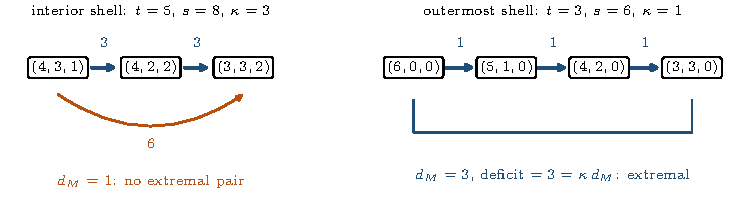
\includegraphics{fig-rigidity}
\caption{The concatenation obstruction of
Theorem~\ref{thm:pair-rigidity}, in $d=3$.  Left, an interior shell: the
two consecutive arcs are minimizing, yet their endpoints already lie at
transfer distance one, so the chain is not a geodesic and the pair is not
extremal.  Right, an outermost shell: the two-coordinate path is a geodesic
whose every segment is minimizing, and equality
in~\eqref{eq:pair-equality} persists at all distances.  Arrow labels are
lens deficits.}
\label{fig:rigidity}
\end{figure}

The simultaneous two-radius order of Theorem~\ref{thm:cross-majorization}
lifts to a whole cone of Lee-radial correlations, together with an exact
criterion for equality in terms of the support of the mixed differences of
the profile.  That lifting uses none of the sharp theory below and is
deferred to Appendix~\ref{app:radial}.

\section{Cubes, capped cross-polytopes, and mixed sums}
\label{sec:polytope-phases}

Corollary~\ref{cor:general-majorization} fixes the sign for every convex
hyperoctahedral body.  It does not determine the smallest positive exposure
sum.  We now evaluate a second sharp family and then show two ways in which
the quantitative layer changes between the cross-polytope and cube.

\subsection{Integer cubes}

The product factorization below is elementary; the new point is its sharp
optimization over the fixed-shell transfer graph.

For $t\in\Z_{\ge0}$, let
\[
 Q_t^d=[-t,t]^d\cap\Z^d.
\]
For $p,q\in\Z_{\ge0}$ and $k\in\Z_{\ge0}$, put
\begin{equation}
 \ell_{p,q}(k)=
 \begin{cases}
  2\min\{p,q\}+1,&0\le k\le|p-q|,\\
  p+q+1-k,&|p-q|<k\le p+q,\\
  0,&k>p+q.
 \end{cases}
 \label{eq:cube-one-dimensional-overlap}
\end{equation}

\begin{theorem}[Cube product kernel and sharp shell constant]
\label{thm:cube-sharp}
For $u\in\Z^d$,
\begin{equation}
 g_{Q_p^d,Q_q^d}(u)
 =\prod_{i=1}^d\ell_{p,q}(|u_i|).                    \label{eq:cube-product}
\end{equation}
The sequence $\ell_{p,q}$ is nonnegative and log-concave on its support, so
for $a,b\in\Z_{\ge0}$ with $a\ge b+2$ the local factor satisfies
\begin{equation}
 \ell_{p,q}(a-1)\ell_{p,q}(b+1)
 -\ell_{p,q}(a)\ell_{p,q}(b)\ge0.                   \label{eq:cube-local}
\end{equation}

 For equal cubes with $t\in\Z_{\ge1}$, let
 $\kappa^\square_{d,t,s}$ be the least unit-transfer arc weight on the shell
 $\mathcal P_d(s)$, for $s\in\Z_{\ge2}$, and put $H=2t+1$.  Then
\begin{equation}
 \kappa^\square_{2,t,s}=
 \begin{cases}1,&s\le H,\ s\ \text{even},\\
              2,&s\le H,\ s\ \text{odd},\\
              0,&s\ge H+1,\end{cases}
 \qquad
 \kappa^\square_{d,t,s}=
 \begin{cases}(H+2-s)H^{d-3},&2\le s\le H,\\
              0,&s\ge H+1,\end{cases}
 \quad(d\ge3).                                      \label{eq:cube-kappa}
\end{equation}
Thus the active shells of the equal-radius cube are exactly
$2\le s\le2t+1$, one layer beyond the Lee support bound $2t$.
For $d\ge3$ and $2\le s\le H$ the minimum is attained, modulo signed
permutations, by the canonical axial-residual edge of
Definition~\ref{def:axial-edge},
\begin{equation}
 \operatorname{sort}(s-2,2,0^{d-2})
 \longrightarrow
 \operatorname{sort}(s-2,1,1,0^{d-3}).              \label{eq:cube-minimizer}
\end{equation}
Consequently, for comparable $\lambda\succeq\mu$ on the shell,
\[
 g_{Q_t^d,Q_t^d}(\mu)-g_{Q_t^d,Q_t^d}(\lambda)
 \ge\kappa^\square_{d,t,s}d_M(\lambda,\mu),
\]
and the coefficient is sharp.
\end{theorem}

\begin{proof}
The one-dimensional overlap of $[-p,p]\cap\Z$ and its translate by $-k$ is
~\eqref{eq:cube-one-dimensional-overlap}; coordinate independence gives
~\eqref{eq:cube-product}.  For~\eqref{eq:cube-local}, suppose first that all
four arguments lie in the support $[0,p+q]$.  There the sequence is constant
and then decreases linearly, so the adjacent ratio
$\ell_{p,q}(k+1)/\ell_{p,q}(k)$ equals one on the flat part and
$1-1/(p+q+1-k)$ on the linear part, hence is nonincreasing in $k$.  Since
$a-1\ge b+1$,
\[
 \frac{\ell_{p,q}(a)}{\ell_{p,q}(a-1)}
 \le\frac{\ell_{p,q}(b+1)}{\ell_{p,q}(b)},
\]
and cross-multiplying the positive denominators gives~\eqref{eq:cube-local}.
The zero boundary is handled by the zero extension: if $\ell_{p,q}(a)=0$ or
$\ell_{p,q}(b)=0$, the subtracted product vanishes and the inequality is
immediate, while $\ell_{p,q}(a-1)=0$ forces $a-1>p+q$ and hence
$\ell_{p,q}(a)=0$ as well.

For equal radii and $2\le s\le H$, every coordinate of a nonnegative shell
representative satisfies $u_i\le s\le H$, so each clipped factor equals
$H-u_i\ge0$ (a factor may vanish at $u_i=H$) and
\[
 g_{Q_t^d,Q_t^d}(u)=\prod_i(H-u_i).
\]
A transfer on coordinates $(a,b)$
with $D=a-b\ge2$ has exact weight
\begin{equation}
 (D-1)\prod_{k\ne i,j}(H-u_k),                       \label{eq:cube-edge-weight}
\end{equation}
because
$(H-a+1)(H-b-1)-(H-a)(H-b)=D-1$; the formula $\ell_{t,t}(k)=H-k$ remains
valid throughout $0\le k\le H$, with its zero endpoint at $k=H$ supplied by
the zero extension in~\eqref{eq:cube-one-dimensional-overlap}, so all four
factors are covered.

Assume $d\ge3$, and let the untouched coordinates have total mass
$q=s-a-b$.  Repeatedly applying
\[
 (H-x)(H-y)\ge H(H-x-y)
 \qquad(x,y\ge0),
\]
which holds because the difference of the two sides is $xy$,
concentrates this mass and gives
\[
 \prod_{k\ne i,j}(H-u_k)
 \ge H^{d-3}(H-q)=H^{d-3}(H-s+a+b).
\]
Since $a+b\ge D\ge2$ and $H-s\ge0$,
\[
 (D-1)(H-s+a+b)\ge H-s+2>0.
\]
Equality requires $D=a+b=2$ and all untouched mass in at most one coordinate;
the arc~\eqref{eq:cube-minimizer} has exactly this form, and its untouched
coordinate $s-2\le H$ stays inside the support.  This proves the
$d\ge3$ formula on $2\le s\le H$.  For $d=2$ the residual product is empty
and $D$ has the parity of $s$; its least admissible value is two on even
shells and three on odd shells, attained by the balanced edges
$(s/2+1,s/2-1)\to(s/2,s/2)$ and
$((s+3)/2,(s-3)/2)\to((s+1)/2,(s-1)/2)$, whose coordinates stay at most
$H$ for $s\le H$.

Finally let $s\ge H+1$.  Both endpoints of the arc
$(s,0^{d-1})\to(s-1,1,0^{d-2})$ leaving the axial composition $se_1$ have
first coordinate at least $H$, so the
clipped product~\eqref{eq:cube-product} vanishes at both endpoints and the
arc weight is zero.  Every arc weight is nonnegative by
Corollary~\ref{cor:general-majorization}, whence
$\kappa^\square_{d,t,s}=0$.  Telescoping along a shortest unit-transfer path
proves the final stability statement, and an attaining arc proves sharpness.
\end{proof}

The equality analysis inside the proof is already complete enough to
classify all minimizers, and the outcome is the exact opposite of the Lee
degeneracy in Theorem~\ref{thm:arc-classification}.

\begin{corollary}[Rigidity of the cube sharp layer]
\label{cor:cube-arc-classification}
Let $d\ge3$, $t\ge1$, and $2\le s\le H=2t+1$.  Modulo signed permutations,
the canonical axial-residual edge~\eqref{eq:cube-minimizer} is the
\emph{only} arc of $\mathcal P_d(s)$ attaining $\kappa^\square_{d,t,s}$.
For $d=2$ the unique minimizer is the balanced arc listed in the proof
above.
\end{corollary}

\begin{proof}
On an active shell every untouched coordinate satisfies
$u_k\le s-a-b\le s-2\le H-2$, so all factors of
~\eqref{eq:cube-edge-weight} are at least two, and the weight is the exact
product $(D-1)\prod_{k\ne i,j}(H-u_k)$.  The chain in the proof bounds this
below by $(D-1)H^{d-3}(H-s+a+b)\ge H^{d-3}(H-s+2)$.  Equality in the first
step forces $u_ku_l=0$ for every pair of untouched coordinates, that is, a
concentrated residual; equality in the second step forces $D=a+b=2$, since
$D=2<a+b$ gives $(H-s+a+b)>(H-s+2)$ and $D\ge3$ gives
$(D-1)(H-s+a+b)\ge2(H-s+3)>H-s+2$.  The remaining data $(a,b)=(2,0)$ and
$w=(s-2)e_1$ describe exactly the arc~\eqref{eq:cube-minimizer}.  For
$d=2$ the weight is $D-1$, which is uniquely minimized by the least
admissible gap of the correct parity.
\end{proof}

Thus, on every interior Lee shell the sharp layer carries
$\lfloor s/2\rfloor-1$ arcs, whereas the cube sharp layer is a single arc on
\emph{all} of its active shells: two solved models with the same universal
transfer sign, the same attaining canonical edge, and entirely different
extremal degeneracy.

\subsection{Capped cross-polytopes}

For integers $c,t\ge1$ with $t\le2c$, define
\[
 P_{t,c}^{(2)}
 =\{x\in\Z^2:\|x\|_1\le t,\ \|x\|_\infty\le c\}.
\]
This is the Lee ball when $t\le c$ and the full cube $[-c,c]^2\cap\Z^2$
when $t=2c$.  The next proposition tracks one distinguished atomic
increment as the body interpolates from cross-polytope to cube; it does not
compute a shell constant.

\begin{proposition}[Exact tent-shaped transfer magnitude]
\label{prop:capped-crossover}
For the first balancing arc,
\begin{equation}
 g_{P_{t,c}^{(2)},P_{t,c}^{(2)}}(1,1)
 -g_{P_{t,c}^{(2)},P_{t,c}^{(2)}}(2,0)
 =\min\{2t-1,\ 4c-2t+1\}.                            \label{eq:capped-tent}
\end{equation}
Thus the increment increases with slope two through $t=c$, has the common
maximum $2c-1$ at $t=c$ and $t=c+1$, and then decreases with slope minus two;
it remains positive throughout.  Figure~\ref{fig:sharp-constants} plots this
tent alongside the Lee and cube constants.
\end{proposition}

\begin{proof}
Under $(x,y)\mapsto(r,w)=(x+y,x-y)$, the body becomes the parity-lattice
points satisfying
\[
 |r|\le t,\qquad |w|\le t,\qquad |r|+|w|\le2c.
\]
For the arc $(2,0)\to(1,1)$, the coordinate sum shift remains two and the
difference shift changes from two to zero.  For $|r|\le t$, let
\[
 m(r)=\max\{m\in\Z_{\ge0}:m\equiv r\pmod2,\ m\le t,\ |r|+m\le2c\},
\]
and leave $m(r)$ undefined when the fiber is empty.  The two coordinate-sum
fibers are indexed by $r$ and $r+2$, so their endpoints have the same parity.
With $D=2$, Lemma~\ref{lem:atomic-exposure} says that the fiber exposure is one
exactly when both fibers are nonempty and $m(r)=m(r+2)$.  Comparing the two
clipped endpoints gives
\begin{equation}
 r\in\mathcal R
 =[-t,t-2]\cap[t-2c-1,\,2c-t-1]\cap\Z.              \label{eq:capped-active-r}
\end{equation}
The two integer intervals have respectively $2t-1$ and $4c-2t+1$ points.
The first is contained in the second when $t\le c$, and the second is
contained in the first when $t\ge c+1$.  Hence
$|\mathcal R|$ is the right-hand side of~\eqref{eq:capped-tent}.
\end{proof}

\begin{figure}[htbp]
\centering
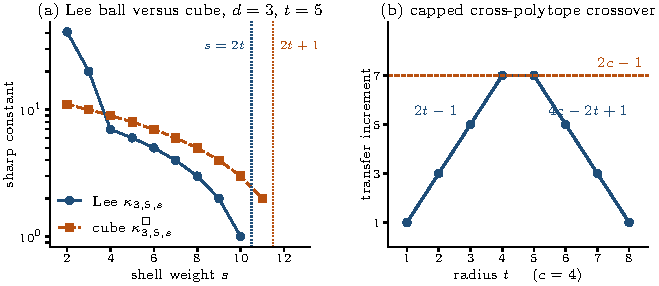
\includegraphics{fig-sharp-constants}
\caption{Quantitative profiles of the two comparisons of this section.
Panel~(a) plots the Lee constant $\kappa_{3,5,s}$ of
Theorem~\ref{thm:sharp-kappa} against the cube constant
$\kappa^\square_{3,5,s}$ of~\eqref{eq:cube-kappa} on a logarithmic scale:
the cube decays linearly and stays active one shell longer, while the Lee
constant drops steeply off the two innermost shells.  Panel~(b) plots the
tent of~\eqref{eq:capped-tent} for $c=4$, with the two linear branches
meeting at the plateau $2c-1$ carried by $t=c$ and $t=c+1$.}
\label{fig:sharp-constants}
\end{figure}

\subsection{A mixed Minkowski family}

Recall $C_3=\{x\in\R^3:\|x\|_1\le1\}$ and let
$B_\infty^3=[-1,1]^3$.  For
$b\in\Z_{\ge1}$, put
\[
 K_b=C_3+bB_\infty^3,\qquad A_b=K_b\cap\Z^3.
\]
Equivalently,
\begin{equation}
 A_b=\left\{x\in\Z^3:
 \sum_{i=1}^3(|x_i|-b)_+\le1\right\}.                \label{eq:mixed-membership}
\end{equation}
Write $N=2b+1$ and $S=2(b+1)=N+1$.

\begin{theorem}[Mixed outer-shell constants and a noncanonical sharp family]
\label{thm:mixed-sharp}
For $s\in\Z_{\ge2}$, put
\begin{equation}
 \kappa^{\mathrm{mix}}_b(s)
 =\min_{\lambda\to\mu\text{ in }\mathcal P_3(s)}
 \bigl(g_{A_b,A_b}(\mu)-g_{A_b,A_b}(\lambda)\bigr).   \label{eq:mixed-kappa-def}
\end{equation}
Then
\begin{equation}
 \kappa^{\mathrm{mix}}_b(S)=5,\qquad
 \kappa^{\mathrm{mix}}_b(S+1)=4,\qquad
 \kappa^{\mathrm{mix}}_b(s)=0\quad(s\ge S+2).         \label{eq:mixed-kappa}
\end{equation}
On $\mathcal P_3(S)$ the unique minimizing unit-transfer arc modulo signed
permutations is
\begin{equation}
 \operatorname{sort}(2b-2,3,1)
 \longrightarrow
 \operatorname{sort}(2b-2,2,2),                     \label{eq:mixed-minimizer}
\end{equation}
and on $\mathcal P_3(S+1)$ the minimum is attained by
\begin{equation}
 \operatorname{sort}(2b-1,3,1)
 \longrightarrow
 \operatorname{sort}(2b-1,2,2).                     \label{eq:mixed-minimizer-outer}
\end{equation}
The arc~\eqref{eq:mixed-minimizer-outer} is the unique minimizer for
$b\ge2$; for $b=1$ exactly one further arc, $(3,2,0)\to(3,1,1)$, also has
weight four.  Hence the outermost active shell of the family is
$S+1=2b+3$: the sharp constant decreases from five to four on the last two
active shells and then vanishes.  For every $b$ the minimizing arc on
$\mathcal P_3(S)$ lies outside the signed-permutation orbit of the
canonical axial-residual edge of Definition~\ref{def:axial-edge}, and for
$b\ge2$ so does the minimizing arc on
$\mathcal P_3(S+1)$.  In particular, this infinite family does not have the
canonical axial-residual sharp edge shared by the Lee and cube formulas.
\end{theorem}

\begin{proof}
Put
\[
 Q_b=\{-b,\ldots,b\},\qquad E_b=\{-b-1,b+1\},\qquad
 \mathcal S=\{000,100,010,001\}.
\]
The membership condition~\eqref{eq:mixed-membership} gives the disjoint
four-state decomposition
\[
 A_b=\bigsqcup_{\alpha\in\mathcal S}
 S_{\alpha_1}\times S_{\alpha_2}\times S_{\alpha_3},
 \qquad S_0=Q_b,\quad S_1=E_b.
\]
Let $M_k(\alpha,\beta)=|S_\alpha\cap(S_\beta-k)|$.  Exact interval
intersection gives
\begin{equation}
 M_0=\begin{pmatrix}N&0\\0&2\end{pmatrix},\qquad
 M_k=\begin{pmatrix}N-k&1\\1&0\end{pmatrix}\quad(1\le k\le N),\qquad
 M_{N+1}=\begin{pmatrix}0&0\\0&1\end{pmatrix},        \label{eq:mixed-matrices}
\end{equation}
and $M_k=0$ for $k\ge N+2$.  The generic matrix remains valid up to $k=N$
inclusive, where its corner entry vanishes; only the coordinate shifts
$N+1$ and beyond are exceptional, and we flag every use of the boundary
matrix $M_{N+1}$ below.  Consequently
\begin{equation}
 g_{A_b,A_b}(u)=
 \sum_{\alpha,\beta\in\mathcal S}
 \prod_{i=1}^3M_{u_i}(\alpha_i,\beta_i).             \label{eq:mixed-state-sum}
\end{equation}

\emph{Case exhaustion.}  After signed permutation and sorting, every
unit-transfer edge on $\mathcal P_3(s)$ is described by a donor coordinate, a
recipient coordinate exceeded by the donor by at least two, and one untouched
coordinate.  Either the recipient is positive---then both transfer
coordinates are positive and the untouched coordinate is positive or
zero---or the recipient is zero, and the donor and the untouched coordinate
carry the whole shell mass.  These two cases are treated separately below on
each shell and exhaust the transfer graph.

\emph{The generic transfer difference.}  Suppose the transfer acts on two
positive coordinates $a>c\ge1$, has gap $D=a-c\ge2$, leaves untouched
coordinate $r\ge0$, and suppose every coordinate of $u$ and of $u'$ lies in
$\{0,1,\ldots,N\}$.  When all three shift coordinates are positive, put
$A_i=N-u_i\ge0$; expanding~\eqref{eq:mixed-state-sum} over the sixteen state
pairs reduces the state sum to
\begin{equation}
 G(u)=A_1A_2A_3
 +2(A_1A_2+A_1A_3+A_2A_3)
 +2(A_1+A_2+A_3).                                    \label{eq:mixed-generic-sum}
\end{equation}
If the untouched coordinate is zero, the entries $M_0(0,1)=M_0(1,0)=0$
remove the mixed terms in that coordinate while $M_0(0,0)=N$ and
$M_0(1,1)=2$ give
\begin{equation}
 g_{A_b,A_b}(a,c,0)
 =N\bigl[A_aA_c+2(A_a+A_c)+2\bigr]+2A_aA_c,          \label{eq:mixed-zero-residual-sum}
\end{equation}
with $A_a=N-a$ and $A_c=N-c$.  Direct subtraction in either case yields
\begin{equation}
 \Delta=(N-r+2)(D-1),                                \label{eq:mixed-positive-pair}
\end{equation}
valid on every shell on which the stated coordinate bounds hold.

\emph{The shell $S=N+1$.}  If both transfer coordinates are positive, then
$a\le S-c-r\le N$, so~\eqref{eq:mixed-positive-pair} applies with
$N-r+2=a+c+1\ge5$, because $a\ge c+2$ and $c\ge1$ force $a+c\ge4$.
Equality holds exactly when $(a,c)=(3,1)$ and $r=S-4=2b-2$, which gives
~\eqref{eq:mixed-minimizer}.

For a transfer into a zero coordinate, write the source as $(a,r,0)$ with
donor $a\ge2$, untouched coordinate $r$, and $a+r=S$.  For $r=0$ the source
$(N+1,0,0)$ uses the boundary matrix $M_{N+1}$, which forces the first
coordinate into the state pair $(1,1)$ and gives
$g_{A_b,A_b}(N+1,0,0)=N^2$; the target $(N,1,0)$ is generic.  For $r\ge1$
both endpoints are covered by~\eqref{eq:mixed-generic-sum} and
~\eqref{eq:mixed-zero-residual-sum}.  The same state sums give
\begin{equation}
 \Delta=
 \begin{cases}
  N^2,&r=0,\\
  (N-1)(N+3),&r=1,\\
  a^2+2N-3,&r\ge2.
 \end{cases}                                         \label{eq:mixed-zero-recipient}
\end{equation}
Every value is at least seven for $N\ge3$.  Therefore the value five in
~\eqref{eq:mixed-positive-pair} is the unique minimum on $\mathcal P_3(S)$.

\emph{The shell $S+1=N+2$.}  Suppose first that both transfer coordinates
are positive.  If the untouched coordinate satisfies $r\ge1$, then
$a\le N$, formula~\eqref{eq:mixed-positive-pair} applies, and now
$r=N+2-a-c$ gives $N-r+2=a+c$, so
\begin{equation}
 \Delta=(a+c)(a-c-1)\ge4\cdot1=4,                    \label{eq:mixed-outer-generic}
\end{equation}
with equality exactly when $a+c=4$ and $a-c=2$, that is $(a,c)=(3,1)$ and
$r=N-2=2b-1$; this is the arc~\eqref{eq:mixed-minimizer-outer}.  If instead
$r=0$, then $a+c=N+2$.  For $c\ge2$ all coordinates stay in the generic
range and~\eqref{eq:mixed-positive-pair} gives
$\Delta=(N+2)(D-1)\ge N+2\ge5$.  For $c=1$ the source is $(N+1,1,0)$: the
boundary matrix $M_{N+1}$ forces its first coordinate into the state pair
$(1,1)$ and gives $g_{A_b,A_b}(N+1,1,0)=N(N-1)$, while
~\eqref{eq:mixed-zero-residual-sum} gives $g_{A_b,A_b}(N,2,0)=2N(N-1)$;
hence $\Delta=N(N-1)\ge6$.

Next consider a transfer into a zero coordinate, with source $(a,r,0)$,
donor $a\ge2$, untouched coordinate $r$, and $a+r=N+2$.  For $r=0$ the source
$(N+2,0,0)$ has a coordinate shift of $N+2$, so its state sum vanishes, and
the target value $g_{A_b,A_b}(N+1,1,0)=N(N-1)$ computed above gives
$\Delta=N(N-1)\ge6$.  For $r=1$ the source is again $(N+1,1,0)$ with value
$N(N-1)$, and the generic target value
$g_{A_b,A_b}(N,1,1)=2(N-1)(N+1)$ from~\eqref{eq:mixed-generic-sum} gives
$\Delta=(N-1)(N+2)\ge10$.  For $2\le r\le N$ both endpoints are generic;
substituting $A_a=r-2$, $A_r=N-r$ into~\eqref{eq:mixed-zero-residual-sum}
and $(A_1,A_2,A_3)=(r-1,N-r,N-1)$ into~\eqref{eq:mixed-generic-sum} yields
\begin{equation}
 \Delta=(N-r)(N-r+3)+2(N-1)\ge2(N-1),                \label{eq:mixed-outer-zero-recipient}
\end{equation}
with equality exactly at $r=N$, since the first summand is strictly
decreasing in $r$.  For $b\ge2$ one has $2(N-1)\ge8>4$, so
~\eqref{eq:mixed-minimizer-outer} is the unique minimizer.  For $b=1$
(so $N=3$) the value $2(N-1)=4$ is attained exactly at $r=N=3$, that is by
the single further arc $(3,2,0)\to(3,1,1)$.  This proves
$\kappa^{\mathrm{mix}}_b(S+1)=4$ together with the stated minimizers.

\emph{Shells $s\ge S+2$.}  Both endpoints of the arc
$(s,0,0)\to(s-1,1,0)$ leaving the axial composition $se_1$ have first
coordinate at least $N+2$, so $M_{u_1}=0$
annihilates every state product and both covariogram values vanish; the arc
weight is zero.  Since $A_b$ is the lattice section of a compact convex set
invariant under signed coordinate permutations,
Corollary~\ref{cor:general-majorization} makes every arc weight nonnegative,
whence $\kappa^{\mathrm{mix}}_b(s)=0$.
\end{proof}

At axial radius two, the three nonnegative integer coefficient pairs in
\[
 \alpha C_3+\beta B_\infty^3,
 \qquad \alpha+\beta=2,
\]
can be compared on the same shell $s=4$.
The values and minimizing orbits are listed in
Table~\ref{tab:polytope-phase}: the first row follows from
Theorem~\ref{thm:cube-sharp}, the second from
Theorem~\ref{thm:mixed-sharp}, and the last from the Lee values
$1,2,3,4$ at $(4,0,0),(3,1,0),(2,2,0),(2,1,1)$.
\par
\begin{table}[ht]
\centering
\caption{A fixed-scale quantitative transition on $\mathcal P_3(4)$.  The
transfer sign stays positive, while the sharp constant and minimizing orbit
change.}
\label{tab:polytope-phase}
\small
\begin{tabular}{lccp{6.0cm}}
\toprule
body & $(\alpha,\beta)$ & $\kappa$ & minimizing unit-transfer orbit(s)\\
\midrule
$2B_\infty^3$ & $(0,2)$ & $3$ &
$(2,2,0)\to(2,1,1)$\\
$C_3+B_\infty^3$ & $(1,1)$ & $5$ &
$(3,1,0)\to(2,2,0)$\\
$2C_3$ & $(2,0)$ & $1$ &
$(4,0,0)\to(3,1,0)$,\;
$(3,1,0)\to(2,2,0)$,\;
$(2,2,0)\to(2,1,1)$\\
\bottomrule
\end{tabular}
\end{table}
Thus even at fixed dimension, scale, and shell, the sharp extremizer is not
universal.  The next section replaces this observation by an exact threshold.
\FloatBarrier

\section{Structural evaluation and facet threshold}
\label{sec:structural}

In each of the three families solved above, the sharp constant is attained
inside one explicit set of arcs, indexed by the recipient coordinate: the
gap-two transfers whose residual mass $c$ sits in a single coordinate.  Those
with $c\ge2$ are the balanced-gap axial family of
Definition~\ref{def:balanced-family}, and $c\in\{0,1\}$ is its boundary
continuation.  Equal Lee balls select
\emph{every} member of that family on every interior shell
(Theorem~\ref{thm:arc-classification}); equal cubes select the single member
with recipient zero, that is the canonical axial-residual edge
(Corollary~\ref{cor:cube-arc-classification}); and the mixed body
$C_3+bB_\infty^3$ selects the member with recipient one
(Theorem~\ref{thm:mixed-sharp}).  This section evaluates the mixed family in
every dimension, on every shell that avoids the outer boundary layer, and
shows that which member is selected is decided by one inequality between the
dimension and the geometry of the body.  We locate that facet threshold
exactly.

Throughout, for $d\ge1$ and $b\in\Z_{\ge1}$ put
\[
 A_b^{(d)}=\bigl(C_d+bB_\infty^d\bigr)\cap\Z^d
 =\Bigl\{x\in\Z^d:\sum_{i=1}^d(|x_i|-b)_+\le1\Bigr\},
 \qquad
 g_b^{(d)}=g_{A_b^{(d)},A_b^{(d)}},
\]
so that $A_b^{(3)}=A_b$ is the body of Theorem~\ref{thm:mixed-sharp}, and
write
\[
 N=2b+1,\qquad e=d-2.
\]
All shifts below are nonnegative, as we may assume after a signed
permutation.

\subsection{The master kernel}

The four-state decomposition used for $d=3$ collapses, in every dimension, to
a single polynomial in the coordinatewise interval overlaps.  Everything in
this section is computed from it.

\begin{lemma}[Master kernel]
\label{lem:master-kernel}
Let $d\ge1$, $b\ge1$, and let $u\in\Z_{\ge0}^d$ satisfy $u_i\le N$ for every
$i$.  Put $m_i=N-u_i\ge0$.  Then
\begin{equation}
 g_b^{(d)}(u)
 =\prod_{i=1}^dm_i
 +2\sum_{j=1}^d\prod_{i\ne j}m_i
 +\sum_{\substack{j\ne k\\u_j\ge1,\ u_k\ge1}}\prod_{i\ne j,k}m_i,
 \label{eq:master-kernel}
\end{equation}
the last sum running over ordered pairs.  In particular $g_b^{(d)}(u)>0$
whenever $u_i<N$ for every $i$.
\end{lemma}

\begin{proof}
The membership condition $\sum_i(|x_i|-b)_+\le1$ says that at most one
coordinate leaves the central range $Q_b=\{-b,\ldots,b\}$, and that it then
lies in $E_b=\{-(b+1),b+1\}$.  With $S_0=Q_b$, $S_1=E_b$, and
$\mathcal S=\{\varepsilon\in\{0,1\}^d:\sum_i\varepsilon_i\le1\}$, this is the
disjoint decomposition
\[
 A_b^{(d)}=\bigsqcup_{\varepsilon\in\mathcal S}
 S_{\varepsilon_1}\times\cdots\times S_{\varepsilon_d}.
\]
Sorting the points of $A_b^{(d)}\cap(A_b^{(d)}-u)$ by the block containing
$x$ and the block containing $x+u$ gives
\begin{equation}
 g_b^{(d)}(u)
 =\sum_{\varepsilon,\eta\in\mathcal S}
 \prod_{i=1}^dM_{u_i}(\varepsilon_i,\eta_i),
 \qquad
 M_k(\varepsilon,\eta)=|S_\varepsilon\cap(S_\eta-k)|.
 \label{eq:master-state-sum}
\end{equation}
Exact interval intersection evaluates these one-dimensional kernels: for
$0\le k\le N$,
\[
 M_k(0,0)=N-k,\qquad
 M_k(0,1)=M_k(1,0)=\mathbf 1[k\ge1],\qquad
 M_k(1,1)=2\cdot\mathbf 1[k=0].
\]
Indeed $b+1-k\in Q_b$ exactly for $1\le k\le N$, which gives the two mixed
entries, while $E_b\cap(E_b-k)$ is empty unless $k=0$ or $k=N+1$.

Each $\varepsilon\in\mathcal S$ is either $0$ or a standard basis vector, so
~\eqref{eq:master-state-sum} has exactly four types of term.  The pair
$\varepsilon=\eta=0$ contributes $\prod_im_i$.  The three types with support
in a single coordinate $j$ contribute
\[
 \bigl(M_{u_j}(1,0)+M_{u_j}(0,1)+M_{u_j}(1,1)\bigr)\prod_{i\ne j}m_i
 =2\prod_{i\ne j}m_i,
\]
because the bracket equals $2$ both when $u_j\ge1$ and when $u_j=0$, so one
formula covers zero and positive coordinates alike.  The
remaining terms have $\varepsilon=e_j$, $\eta=e_k$ with $j\ne k$ and
contribute $\mathbf 1[u_j\ge1]\mathbf 1[u_k\ge1]\prod_{i\ne j,k}m_i$.
Summing the four types gives~\eqref{eq:master-kernel}.  If $u_i<N$ for every
$i$, then every $m_i\ge1$ and the first product is already positive.
\end{proof}

For $e\ge1$ and $0\le r\le N$ write
\begin{equation}
 \Gamma_b^{(e)}(r)=g_b^{(e)}(re_1)
 =(N+2-r)N^{e-1}+2(e-1)(N-r)N^{e-2},
 \label{eq:gamma}
\end{equation}
the second term being absent when $e=1$; this is the self-overlap of the same
body \emph{two dimensions down}, at the concentrated shift $re_1$.  It is
strictly decreasing in $r$ on $\{0,\ldots,N\}$, with
\begin{equation}
 \Gamma_b^{(e)}(r)-\Gamma_b^{(e)}(r+2)=2N^{e-1}+4(e-1)N^{e-2}.
 \label{eq:gamma-step}
\end{equation}

\subsection{The edge law}

Every unit transfer now falls into one of exactly two regimes, according to
whether the recipient coordinate is positive or zero.  The first regime obeys
a clean factorization; the second pays an explicit surcharge.

\begin{lemma}[Edge law]
\label{lem:edge-law}
Let $d\ge2$, $b\ge1$, and let $u\in\Z_{\ge0}^d$ have all coordinates at most
$N$.  Let the transfer act on a donor $a=u_1$ and a recipient $c=u_2$ with
$a\ge c+2$, put $D=a-c$, let $w=(u_3,\ldots,u_d)$ be the residual, and set
$u'=u-e_1+e_2$.  Assume also $u_1'=a-1\le N$ and $u_2'=c+1\le N$.  Put
\begin{equation}
 P(w)=\prod_{i=1}^em_i,\qquad
 F(w)=\sum_{j:\,w_j\ge1}\ \prod_{i\ne j}m_i,\qquad m_i=N-w_i,
 \label{eq:residual-functionals}
\end{equation}
with the conventions $g_b^{(0)}(0)=P=1$ for the empty products and $F=0$ for
the empty sum when $e=0$.  Then
\begin{equation}
 g_b^{(d)}(u')-g_b^{(d)}(u)
 =\begin{cases}
  (D-1)\,g_b^{(e)}(w),&c\ge1,\\[4pt]
  (a-1)\,g_b^{(e)}(w)+2P(w)+2(N-a)F(w),&c=0.
 \end{cases}
 \label{eq:edge-law}
\end{equation}
\end{lemma}

\begin{proof}
Split the three sums of~\eqref{eq:master-kernel} according to how many of the
two indices $j,k$ lie in $\{1,2\}$.  Write $E_1=\sum_{j}\prod_{i\ne j}m_i$
and $E_2=\sum_{j\ne k,\,w_jw_k\ge1}\prod_{i\ne j,k}m_i$ for the
corresponding residual sums, so that $g_b^{(e)}(w)=P+2E_1+E_2$
by~\eqref{eq:master-kernel} in dimension $e$; for $e=0$ all three residual
quantities are empty, $P=1$ and $E_1=E_2=F=0$, and the identity reads
$g_b^{(0)}(0)=1$.  One obtains
\begin{multline}
 g_b^{(d)}(u)=m_1m_2P+2(m_1+m_2)P+2m_1m_2E_1\\
 +2\mathbf 1[c\ge1]P
 +2\bigl(m_2+m_1\mathbf 1[c\ge1]\bigr)F+m_1m_2E_2,
 \label{eq:master-split}
\end{multline}
where we used $a\ge2$, hence $\mathbf 1[a\ge1]=1$.  The transfer replaces
$(m_1,m_2)=(N-a,N-c)$ by $(m_1+1,m_2-1)$; the sum $m_1+m_2$ is preserved and
\begin{equation}
 (m_1+1)(m_2-1)-m_1m_2=m_2-m_1-1=D-1.
 \label{eq:product-jump}
\end{equation}

If $c\ge1$, both endpoints have $\mathbf 1[c\ge1]=1$, so in
~\eqref{eq:master-split} only the coefficient $m_1m_2$ changes, and by
~\eqref{eq:product-jump} the increment is $(D-1)(P+2E_1+E_2)$, which is the
first line of~\eqref{eq:edge-law}.

If $c=0$, then $m_2=N$ at the source and the target has
$(m_1',m_2')=(N-a+1,N-1)$ with both indicator terms present.  Here
$m_1'm_2'-m_1m_2=(N-a+1)(N-1)-(N-a)N=a-1$ and
$m_1'+m_2'=2N-a=m_1+m_2$.  Subtracting the two instances of
~\eqref{eq:master-split} therefore gives
\[
 (a-1)P+2(a-1)E_1+(a-1)E_2
 +2P+\bigl[2(2N-a)-2N\bigr]F
 =(a-1)g_b^{(e)}(w)+2P+2(N-a)F,
\]
which is the second line.
\end{proof}

The surcharge $2P+2(N-a)F$ carried by a transfer into a zero coordinate is a
facet effect.  It arises from the single entry $M_0(1,1)=2$, that is from the
two extreme layers $x_i=\pm(b+1)$ of the cube summand overlapping
themselves; a coordinate is shifted by zero only at a recipient that is
zero, so no other arc sees it.  This is how the canonical axial-residual
edge, the cheapest arc for the cube, is penalized once a cross-polytope
summand is present.

We also need the elementary fact that a concentrated residual is the cheapest
one, simultaneously for all three functionals appearing
in~\eqref{eq:edge-law}.

\begin{lemma}[Residual monotonicity]
\label{lem:residual-monotone}
Let $e\ge1$ and let $\lambda\succeq\mu$ be distinct nonnegative compositions
of $r$ into $e$ parts with $r\le N-2$.  Then
\[
 g_b^{(e)}(\mu)>g_b^{(e)}(\lambda),\qquad
 P(\mu)\ge P(\lambda),\qquad
 F(\mu)\ge F(\lambda).
\]
Consequently, among all $w\in\Z_{\ge0}^e$ with $\|w\|_1=r\le N-2$ the
concentrated residual $re_1$ minimizes $g_b^{(e)}$, $P$, and $F$
simultaneously, and it is the unique minimizer of $g_b^{(e)}$.
\end{lemma}

\begin{proof}
By the majorization theorem of Hardy--Littlewood--P\'olya, $\mu$ is obtained
from $\lambda$ by a finite chain of unit balancing transfers, so it suffices
to treat one transfer; since $re_1$ majorizes every composition of $r$ into
$e$ parts, the three inequalities then give the last statement.  A transfer
needs $e\ge2$.  All coordinates involved are at most $r\le N-2$,
so every $m_i\ge2$ and Lemma~\ref{lem:edge-law} applies in dimension $e$,
where the residual has dimension $e-2\ge0$.  Its two cases give increments
$(D-1)g_b^{(e-2)}(w)\ge g_b^{(e-2)}(w)>0$ and
$(a-1)g_b^{(e-2)}(w)+2P+2(N-a)F>0$ respectively, using
Lemma~\ref{lem:master-kernel} for positivity and, when $e=2$, the
conventions of Lemma~\ref{lem:edge-law}.  This gives the strict statement for
$g_b^{(e)}$.

For $P$, the transfer multiplies the two active factors and leaves the rest
fixed, so $P$ increases by $(D-1)\prod_{i\ge3}m_i\ge0$ when the recipient is
positive, and by $(a-1)\prod_{i\ge3}m_i\ge0$ when it is zero,
by~\eqref{eq:product-jump} and the computation in the proof of
Lemma~\ref{lem:edge-law}.  For $F$, write $Q=\prod_{i\ge3}m_i$ and
$G=\sum_{j\ge3,\,w_j\ge1}\prod_{i\ge3,\,i\ne j}m_i$.  If the recipient is
positive, then $F=(m_1+m_2)Q+m_1m_2G$ and the increment is $(D-1)G\ge0$.  If
the recipient is zero, then $F=NQ+(N-a)NG$ at the source and
$(2N-a)Q+(N-a+1)(N-1)G$ at the target, so the increment is
$(N-a)Q+(a-1)G\ge0$.
\end{proof}

\subsection{The structural theorem}

\begin{theorem}[Structural evaluation and facet threshold]
\label{thm:structural}
Let $d\ge3$ and $b\ge2$, put $N=2b+1$ and $e=d-2$, and let $s$ satisfy
$4\le s\le N$.  Let
\[
 \kappa_b^{(d)}(s)
 =\min_{\lambda\to\mu\text{ in }\mathcal P_d(s)}
 \bigl(g_b^{(d)}(\mu)-g_b^{(d)}(\lambda)\bigr)
\]
be the least unit-transfer weight on the shell.  Then $\kappa_b^{(d)}(s)$ is
the smaller of the two values
\begin{equation}
 \Gamma_b^{(e)}(s-4)
 \qquad\text{and}\qquad
 \Gamma_b^{(e)}(s-2)+2N^{e-1}(2N-s),
 \label{eq:structural-two-candidates}
\end{equation}
the first being the weight of the balanced-gap arc with recipient one,
\begin{equation}
 \operatorname{sort}(s-4,3,1,0^{d-3})
 \longrightarrow
 \operatorname{sort}(s-4,2,2,0^{d-3}),
 \label{eq:structural-arc-one}
\end{equation}
and the second the weight of the canonical axial-residual edge of
Definition~\ref{def:axial-edge}.  Their difference is governed by the single
quantity
\begin{equation}
 \Theta_{d,b}(s)=N(2N-s-1)-2(d-3),
 \label{eq:threshold}
\end{equation}
namely
\begin{equation}
 \Bigl[\Gamma_b^{(e)}(s-2)+2N^{e-1}(2N-s)\Bigr]-\Gamma_b^{(e)}(s-4)
 =2N^{e-1}(2N-s-1)-4(d-3)N^{e-2},
 \label{eq:threshold-difference}
\end{equation}
which has the sign of $\Theta_{d,b}(s)$.  Consequently, modulo signed
permutations:
\begin{enumerate}
\item if $\Theta_{d,b}(s)>0$, then
 $\kappa_b^{(d)}(s)=\Gamma_b^{(e)}(s-4)$ and the arc
 ~\eqref{eq:structural-arc-one} is the unique minimizer;
\item if $\Theta_{d,b}(s)<0$, then
 $\kappa_b^{(d)}(s)=\Gamma_b^{(e)}(s-2)+2N^{e-1}(2N-s)$ and the canonical
 axial-residual edge is the unique minimizer;
\item if $\Theta_{d,b}(s)=0$, the minimum is attained exactly on these two
 orbits.
\end{enumerate}
In particular every such shell is active, and for comparable
$\lambda\succeq\mu$ on it,
$g_b^{(d)}(\mu)-g_b^{(d)}(\lambda)\ge\kappa_b^{(d)}(s)\,d_M(\lambda,\mu)$
with a sharp constant.
\end{theorem}

\begin{figure}[ht]
\centering
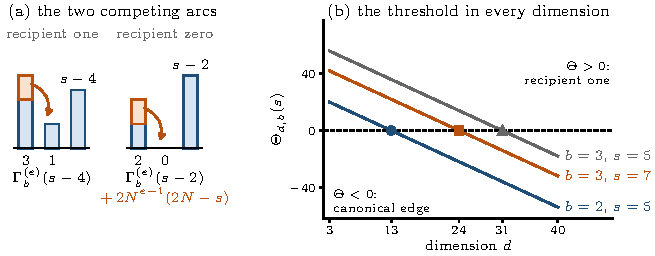
\includegraphics{fig-threshold}
\caption{The competition of Theorem~\ref{thm:structural}.  In (a) the two
candidate arcs of~\eqref{eq:structural-two-candidates}, drawn as donor,
recipient, and residual coordinates with the transferred unit shaded; the
recipient-zero arc buys a larger residual and pays the facet surcharge.  In
(b) the threshold~\eqref{eq:threshold} against the dimension for three pairs
$(b,s)$: it decreases with slope $-2$, and the marked integer zeros
$d=13,24,31$ are the smallest ties, where both arcs are minimizing.}
\label{fig:threshold}
\end{figure}

\begin{proof}
Since $s\le N$, every nonnegative representative of a vertex of
$\mathcal P_d(s)$ has all coordinates at most $s\le N$, so
Lemmas~\ref{lem:master-kernel} and~\ref{lem:edge-law} apply to every arc of
the shell, and the two lines of~\eqref{eq:edge-law} exhaust the arcs.

\emph{Arcs with positive recipient.}  Here $a\ge c+2$ and $c\ge1$ force
$a+c\ge4$, so the residual mass is $\|w\|_1=s-a-c\le s-4\le N-4$.  By
Lemma~\ref{lem:residual-monotone} and the strict monotonicity
~\eqref{eq:gamma-step},
\[
 (D-1)g_b^{(e)}(w)\ \ge\ g_b^{(e)}(w)
 \ \ge\ \Gamma_b^{(e)}(\|w\|_1)
 \ \ge\ \Gamma_b^{(e)}(s-4),
\]
and equality throughout forces $D=2$, $a+c=4$, hence $(a,c)=(3,1)$, together
with a concentrated residual: exactly the arc
~\eqref{eq:structural-arc-one}, whose weight is therefore
$\Gamma_b^{(e)}(s-4)$.

\emph{Arcs with zero recipient.}  Here $D=a$ and
$\|w\|_1=s-a\le s-2\le N-2$; assume first $a\le s-1$, so that $w\ne0$.
By Lemma~\ref{lem:residual-monotone} all three functionals in the second line
of~\eqref{eq:edge-law} are minimized, for fixed $a$, by the concentrated
residual $w=(s-a)e_1$, and strictly so for $g_b^{(e)}$ unless $w$ is
concentrated.  For that residual $P=(N-s+a)N^{e-1}$ and $F=N^{e-1}$, the
latter because exactly one residual coordinate is nonzero, so the surcharge is
\[
 2P+2(N-a)F=2N^{e-1}\bigl[(N-s+a)+(N-a)\bigr]=2N^{e-1}(2N-s),
\]
independent of $a$.  Hence the weight equals
$(a-1)\Gamma_b^{(e)}(s-a)+2N^{e-1}(2N-s)$, and since both $a-1$ and
$\Gamma_b^{(e)}(s-a)$ are positive and strictly increasing in $a$, the
minimum over $2\le a\le s-1$ is attained exactly at $a=2$ with a concentrated
residual, that is exactly at the canonical axial-residual edge, with value
$\Gamma_b^{(e)}(s-2)+2N^{e-1}(2N-s)$.

\emph{The endpoint $a=s$.}  Then $w=0$, so $F$ is an empty sum, $P=N^e$, and
the weight is $(s-1)\Gamma_b^{(e)}(0)+2N^e$ instead of the surcharge form
above.  Since $s\ge4$ and $\Gamma_b^{(e)}$ is positive and strictly
decreasing,
$(s-1)\Gamma_b^{(e)}(0)-\Gamma_b^{(e)}(s-2)>2\Gamma_b^{(e)}(0)\ge2(N+2)N^{e-1}$
by~\eqref{eq:gamma}, so this weight exceeds
$\Gamma_b^{(e)}(s-2)+2N^{e-1}(2N-s)$ by more than
$2(N+2)N^{e-1}+2N^e-2N^{e-1}(2N-s)=2N^{e-1}(s+2)>0$.  Hence the canonical
axial-residual edge minimizes the whole zero-recipient regime.

\emph{Comparison.}  Formula~\eqref{eq:threshold-difference} is
~\eqref{eq:gamma-step} with $r=s-4$, and since $N^{e-2}>0$ its right-hand
side has the sign of $N(2N-s-1)-2(e-1)=\Theta_{d,b}(s)$, which for $e=1$
reduces to $N(2N-s-1)>0$.  The three cases follow, and each candidate value
is positive because $s\le N$, so the shell is active.

For the last statement let $\lambda\succeq\mu$ on the shell.  By
Lemma~\ref{lem:transfer-distance} they are joined by a chain of
$d_M(\lambda,\mu)$ unit balancing transfers, each an arc of the shell.  Every
arc has $g_b^{(d)}$-increment at least $\kappa_b^{(d)}(s)$, so summing along
the chain gives
$g_b^{(d)}(\mu)-g_b^{(d)}(\lambda)\ge\kappa_b^{(d)}(s)\,d_M(\lambda,\mu)$; an
arc attaining the minimum is a comparable pair at distance one for which this
is an equality, so no larger constant works.
\end{proof}

Two features of Theorem~\ref{thm:structural} deserve separate mention.

First, both candidates in~\eqref{eq:structural-two-candidates} are built from
self-overlaps of the same body two dimensions down: the first is such a count
outright, the second is one plus the facet surcharge.  Both previous
evaluations have this shape: the cube constant~\eqref{eq:cube-kappa} is
$(H+2-s)H^{d-3}=g_{Q_t^{d-2},Q_t^{d-2}}\bigl((s-2)e_1\bigr)$ and the first
candidate is $g_b^{(d-2)}\bigl((s-4)e_1\bigr)$, because by
Lemma~\ref{lem:edge-law} and its cube counterpart
~\eqref{eq:cube-edge-weight} an arc with positive recipient weighs $(D-1)$
times the self-overlap of the body in dimension $d-2$ at the residual shift.
The sharp layer is then a $(d-2)$-dimensional enumeration plus the universal
sign of Corollary~\ref{cor:general-majorization} in that dimension, as used in
Lemma~\ref{lem:residual-monotone}.  For the Lee ball the factorization fails
on \emph{every} arc: the increment is the residual convolution of
Proposition~\ref{prop:residual-convolution}, not a product, and the resulting
degeneracy is the family of Theorem~\ref{thm:arc-classification}.

\begin{namedremark}[Three regimes of one family]
Index the gap-two arcs with concentrated residual by the recipient coordinate.
On interior shells equal Lee balls select every member of residual mass at
least two, the whole family of Definition~\ref{def:balanced-family}; equal
cubes select recipient zero; and $C_d+bB_\infty^d$ selects recipient one when
$\Theta_{d,b}(s)>0$ and recipient zero when $\Theta_{d,b}(s)<0$.  The
surcharge $2N^{e-1}(2N-s)$ paid by the recipient-zero arc is of order $N^e$
and comes from the two capped layers of the cube summand; what it buys is the
larger residual mass $s-2$ instead of $s-4$, worth
$2N^{e-1}+4(d-3)N^{e-2}$ by~\eqref{eq:gamma-step}.  Balancing the two
gives~\eqref{eq:threshold}: the facet effect dominates in low dimension, the
$d-3$ free residual coordinates once $2(d-3)$ exceeds $N(2N-s-1)$.  Both signs
occur, and so does the tie: since $N$ is odd, $\Theta_{d,b}(s)=0$ has
solutions exactly for odd $s$, at $d=3+N(2N-s-1)/2$; the smallest are
$(d,b,s)=(13,2,5)$, $(24,3,7)$, $(31,3,5)$, and $(39,4,9)$.
Figure~\ref{fig:threshold} shows the two arcs and the sign change.  For $d=3$
we have $\Theta_{3,b}(s)=N(2N-s-1)>0$ on the whole range, so the
recipient-one arc always wins and~\eqref{eq:gamma} gives the closed form
$\kappa_b^{(3)}(s)=N+6-s$.
\end{namedremark}

\begin{namedremark}[Relation to Theorem~\ref{thm:mixed-sharp} and scope]
For $d=3$ the two evaluations complete each other.  The closed form
$\kappa_b^{(3)}(s)=N+6-s$ covers $4\le s\le N$, and
Theorem~\ref{thm:mixed-sharp} evaluates the two remaining active shells
$s=N+1$ and $s=N+2$, where a coordinate can reach the exceptional shift $N+1$
and the master kernel acquires a boundary correction; its values five and four
are exactly $N+6-s$ there.  So for $d=3$ the constant is $N+6-s$ on every
active shell, with the recipient-one arc minimizing except for the single
additional arc at $b=1$, $s=N+2$.  For $d\ge4$ the hypothesis $s\le N$
confines every coordinate to the range where Lemma~\ref{lem:master-kernel} is
exact; the outer shells are not treated here.
\end{namedremark}

\section{Finite-quotient boundary}
\label{sec:quotient-boundary}

The integer-lattice hypothesis cannot be replaced by a naive finite-$q$
analogue.

\begin{proposition}[Wrap-around order reversal]
In $\Z_6^2$, equip each coordinate with cyclic Lee weight
$|z|_6=\min\{z,6-z\}$ for $z\in\{0,\ldots,5\}$, and take radii $p=1$ and
$q=3$.  Although $(3,1)\succeq(2,2)$, one has
\begin{equation}
 J_{1,3}^{(2),\,\Z_6}(3,1)=3
 >2=J_{1,3}^{(2),\,\Z_6}(2,2).                       \label{eq:qary-reversal}
\end{equation}
\end{proposition}

\begin{proof}
The accepted point sets inside the radius-one ball are
\[
 \{(0,5),(1,0),(5,0)\}
 \qquad\text{and}\qquad
 \{(0,5),(5,0)\},
\]
for the two shifts, respectively.  Their cardinalities prove
\eqref{eq:qary-reversal}.
\end{proof}


\section{Scope and limitations}
\label{sec:limits}

The exact transfer theorem is for finite lattice sets with centered exchange
fibers, and the fixed-shell order additionally requires signed-permutation
invariance.  Lattice sections of compact convex sets invariant under signed
coordinate permutations satisfy both and form a broad sufficient class:
cross-polytopes, cubes, convex symmetric-gauge balls, their intersections, and
their Minkowski sums.  We do not claim the property is necessary; the examples
in~\ref{ex:general-sharpness} show only that dropping convexity or the symmetry
makes a sign reversal possible, not that every set outside the class reverses.

The Lee sharp constant is closed for every
$d\ge2$, while the arc classification and the rigidity need $d\ge3$ and
$4\le s\le2t$, with $s\in\{2,3\}$ separate and $d=2$ uniform.
For $C_d+bB_\infty^d$,
Theorem~\ref{thm:structural} needs $4\le s\le2b+1$; the outer shells
$s>2b+1$ in dimension $d\ge4$, where the master kernel of
Lemma~\ref{lem:master-kernel} acquires boundary corrections, are not treated,
and Theorem~\ref{thm:mixed-sharp} settles them only for $d=3$.  The threshold
$\Theta_{d,b}(s)$ is asserted for this one-parameter family, not for
$\alpha C_d+\beta B_\infty^d$ with $\alpha\ge2$, where
Proposition~\ref{prop:capped-crossover} evaluates one distinguished atomic arc
only.  The symbolic Lee evaluator of Appendix~\ref{app:exact-complexity} is
output-sensitive and pseudopolynomial in the radii; no bound polynomial in the
dimension and the binary-encoded radius is asserted.

The ambient group is the signed-permutation group of the standard integer
lattice; we claim no analogue for an arbitrary lattice basis, and no
finite-$q$ theorem, since~\eqref{eq:qary-reversal} reverses the majorization
order.  The rejection sampling of Remark~\ref{rem:rejection-application} is a
potential application only; its probabilistic assumptions are stated in Online
Resource~1 and used nowhere here.



\section{Conclusion}

For every pair of finite centered exchange-fiber sets, one coordinate
balancing move decomposes exactly into parity-fiber endpoint exposures,
each equal to zero or one; convex hyperoctahedral lattice sections
automatically have these fibers.  It yields a fiberwise equality certificate
along the fixed-shell transfer graph and, for equal Lee balls with $d\ge3$,
the closed sharp constant on every active shell, all minimizing arcs for
$4\le s\le2t$, and the distance-one rigidity of the extremizers on interior
shells.
Cubes factor into interval overlaps, with a product-form
constant.  Section~\ref{sec:structural} locates
all three behaviours inside one mechanism: for $C_d+bB_\infty^d$, an arc with
positive recipient weighs its gap minus one times the self-overlap of the same
body two dimensions down, while an arc into a zero coordinate pays a surcharge
from the two capped layers of the cube summand.  The sharp constant is
therefore determined by lower-dimensional lattice-point counts, with an
explicit facet surcharge
for transfers into a zero coordinate, and which arc realizes it is decided by
the sign of $\Theta_{d,b}(s)$.  Cubes have no surcharge and Lee balls no
factorization, which is why their sharp layers have one and
$\lfloor s/2\rfloor-1$ minimizing arcs: the sign is a matter of symmetry, the
sharp scale and the extremizing geometry are not.

Three problems remain open.  First, the centered exchange-fiber property is
sufficient for the transfer sign but not shown to be necessary; a
characterization of fixed-shell Schur monotonicity by a fiber or exchange
condition would be stronger.  Second, the master kernel of
Lemma~\ref{lem:master-kernel} is special to one cross-polytope summand:
$\alpha C_d+\beta B_\infty^d$ has $\alpha+1$ fiber states, and the exposure
functional replacing the surcharge there would give a two-parameter threshold
surface.  Third, the outer shells $s>2b+1$ with $d\ge4$, where the kernel
acquires boundary corrections, remain open.


\backmatter

\section*{Statements and Declarations}

\subsection*{Funding}
No funding was received for conducting this study.

\subsection*{Competing interests}
The author has no competing interests to declare that are relevant to the
content of this article.

\subsection*{Author contributions}
The sole author designed the study, proved the results, wrote the verification
code, and prepared the manuscript.

\subsection*{Supplementary information}
The article is accompanied by a single supplementary file, Online
Resource~1, containing the probabilistic material behind
Remark~\ref{rem:rejection-application}.  The reproducibility package of
Appendix~\ref{app:repro} is not a supplementary file.

\subsection*{Data availability}
Every numerical value in the tables is regenerated from the source code in the
reproducibility package,
\url{https://github.com/ShunqiLu/covariogram-balancing}, which also supplies
the exact fractions and metadata as CSV, JSON, and Markdown.

\subsection*{Code availability}
The same repository contains the Python source, tests, PowerShell and POSIX
wrappers, LaTeX sources, the figure generator, and a SHA-256 manifest; no
proprietary software or GPU is required.

\begin{appendices}
\renewcommand{\thetable}{\thesection.\arabic{table}}
\renewcommand{\theHtable}{appendix.\thesection.\arabic{table}}

\section{The Lee-radial correlation cone}
\label{app:radial}

The simultaneous two-radius order extends to the Lee-radial correlation
cone
\[
 \mathcal C_{\mathrm{Lee}}
 =\{H:\Z_{\ge0}^2\to\R_{\ge0}:\supp(H)\text{ is finite and }
       \Delta_{12}H\ge0\}.
\]

\begin{theorem}[Order and equality on the Lee-radial correlation cone]
\label{thm:radial-majorization}
Let $H\in\mathcal C_{\mathrm{Lee}}$, with mixed forward differences
\[
 \Delta_{12}H(p,q)=H(p,q)-H(p+1,q)-H(p,q+1)+H(p+1,q+1)\ge0.
\]
Define
\[
 K_H(u)=\sum_{x\in\Z^d}H(\|x\|_1,\|x+u\|_1).
\]
If $\lambda,\mu\in\Z_{\ge0}^d$ have equal coordinate sum and
$\lambda\succeq\mu$, then
\begin{equation}
 K_H(\lambda)\le K_H(\mu).                         \label{eq:radial-schur}
\end{equation}
Moreover, define the lens-equality set
\[
 \mathcal E(\lambda,\mu)=\{(p,q):J_{p,q}^{(d)}(\lambda)=J_{p,q}^{(d)}(\mu)\}.
\]
Then the following equality classification is exact:
\begin{equation}
 K_H(\lambda)=K_H(\mu)
 \quad\Longleftrightarrow\quad
 \supp(\Delta_{12}H)\subseteq\mathcal E(\lambda,\mu). \label{eq:radial-equality}
\end{equation}
In particular, this applies to
$H(r,s)=f(r)g(s)$ for any two nonnegative nonincreasing profiles $f,g$ of
finite support, and by monotone convergence whenever the radial lifts
$x\mapsto f(\|x\|_1)$ and $x\mapsto g(\|x\|_1)$ are summable on $\Z^d$.
Thus, at fixed shift weight $s$, the concentrated (axial) shift $se_1$
minimizes, and the balanced shift---the unique minimal element of the
majorization order on the shell modulo permutations, whose coordinates all
equal $\lfloor s/d\rfloor$ or $\lceil s/d\rceil$---maximizes every
correlation in the cone.

More precisely, for product profiles the inequality is strict for
nonpermutation shifts $\lambda\succeq\mu$ of common weight $s$ whenever
there is an integer $r\ge\lceil s/2\rceil$ such that
\begin{equation}
 f(r)>f(r+1)\quad\hbox{and}\quad g(r)>g(r+1).       \label{eq:radial-strict}
\end{equation}
In particular, for every $0<\sigma,\tau<1$ the correlation
\begin{equation}
 C_{\sigma,\tau}(u)=
 \sum_{x\in\Z^d}\sigma^{\|x\|_1}\tau^{\|x+u\|_1}  \label{eq:lee-geometric-correlation}
\end{equation}
is strictly Schur-concave on each fixed-$\ell_1$-weight class, modulo signed
coordinate permutations.
\end{theorem}

\begin{proof}
Because $H$ has finite support and every Lee shell is finite, all sums in the
finite-support argument are finite.  Double telescoping gives the
lower-orthant decomposition
\[
 H(r,s)=\sum_{p\ge r,q\ge s}\Delta_{12}H(p,q).
\]
Changing the order of summation therefore yields
\[
 K_H(u)=\sum_{p,q\ge0}\Delta_{12}H(p,q)
             J_{p,q}^{(d)}(u).
\]
Theorem~\ref{thm:cross-majorization} applies term by term.  Every summand in
the difference
\[
 K_H(\mu)-K_H(\lambda)=\sum_{p,q\ge0}\Delta_{12}H(p,q)
 \bigl(J_{p,q}^{(d)}(\mu)-J_{p,q}^{(d)}(\lambda)\bigr)
\]
is nonnegative.  Its sum is zero exactly when every positive coefficient
multiplies a zero lens gap, proving~\eqref{eq:radial-equality} for finitely
supported profiles.

For product profiles with infinite support, define the explicit truncations
\[
 f_N(r)=f(r)\,\mathbf 1_{\{r\le N\}},\qquad
 g_N(r)=g(r)\,\mathbf 1_{\{r\le N\}}\qquad(N\in\Z_{\ge0}).
\]
Each truncation is nonnegative and nonincreasing, and
$H_N=f_Ng_N$ has finite support with
\[
 \Delta_{12}H_N(p,q)=(f_N(p)-f_N(p+1))(g_N(q)-g_N(q+1))\ge0,
\]
so the finite-support case applies to every $H_N$.  As $N\to\infty$ the
truncations increase pointwise to $f$ and $g$, hence
$K_{H_N}(u)\uparrow K_H(u)$ by monotone convergence when the radial lifts
are summable, and the weak inequality passes to the limit; Tonelli's theorem
justifies the limiting lower-orthant decomposition, whose resulting
nonnegative series is zero exactly when each positive mixed-difference
coefficient selects a zero lens gap.  Thus the equality criterion also
persists.

For strictness under~\eqref{eq:radial-strict}, fix an integer
$r\ge\lceil s/2\rceil$ with $f(r)>f(r+1)$ and $g(r)>g(r+1)$.  Every
truncated decomposition with $N>r+1$ contains the fixed term
\[
 \bigl(f(r)-f(r+1)\bigr)\bigl(g(r)-g(r+1)\bigr)
 \bigl(J_{r,r}^{(d)}(\mu)-J_{r,r}^{(d)}(\lambda)\bigr),
\]
which is strictly positive by the strict clause of
Theorem~\ref{thm:cross-majorization}, since $s\le2r$.  All other terms are
nonnegative, so the difference $K_H(\mu)-K_H(\lambda)$ is bounded below by
this one positive quantity uniformly in the truncation and remains strictly
positive in the limit.  Taking
$f(r)=\sigma^r$ and $g(r)=\tau^r$ satisfies the summability and strict-drop
conditions at every radius.
\end{proof}

\begin{corollary}[Axial minimizers of Lee-radial correlations]
\label{cor:radial-orbit-reduction}
Let $f:\Z_{\ge0}\to\R_{\ge0}$ be nonincreasing with
$0<Z_f=\sum_{x\in\Z^d}f(\|x\|_1)<\infty$, and let
$g:\Z_{\ge0}\to[0,1]$ be nonincreasing.  Define the normalized Lee-radial
correlation
\[
 A_{f,g}(u)=\frac1{Z_f}
   \sum_{x\in\Z^d}f(\|x\|_1)g(\|x+u\|_1).
\]
If $Y$ has mass $f(\|y\|_1)/Z_f$, then $A_{f,g}(u)$ is the probability that a
radial test with profile $g$ accepts $Y+u$.
For every finite nonempty set $R\subset\Z_{\ge0}$,
\begin{equation}
 \min_{\|u\|_1\in R}A_{f,g}(u)
 =\min_{r\in R}A_{f,g}(re_1).             \label{eq:orbit-reduction}
\end{equation}
Consequently, the minimum of $A_{f,g}$ over $\{u:\|u\|_1\le s\}$ is determined
by the $s+1$ axial values at $0,e_1,\ldots,se_1$.  For a random shift $U$
independent of $Y$ with $\Pr(\|U\|_1\in R)=1$,
\[
 \Pr[\mathrm{accept}]=\E[A_{f,g}(U)]
 \ge\min_{r\in R}A_{f,g}(re_1).
\]
On a fixed shell of weight $s$, if there is an integer
$r\ge\lceil s/2\rceil$ with $f(r)>f(r+1)$ and $g(r)>g(r+1)$, then the axial
signed-permutation orbit is the unique minimizing orbit.
\end{corollary}

\begin{proof}
For a fixed $r$, the vector $re_1$ majorizes the absolute-coordinate vector
of every $u$ with $\|u\|_1=r$.  The radial lift of $g$ need not be summable,
so apply Theorem~\ref{thm:radial-majorization} to the truncated product
profiles $H_N(p,q)=f_N(p)g_N(q)$ of its proof and pass to the limit using
\[
 0\le f(\|x\|_1)g(\|x+u\|_1)\le f(\|x\|_1),\qquad
 \sum_{x\in\Z^d}f(\|x\|_1)=Z_f<\infty,
\]
which dominates all truncations simultaneously.  Division by
$Z_f$ gives
$A_{f,g}(re_1)\le A_{f,g}(u)$ on each shell, with equality attained at
$re_1$.  Taking the minimum over $r\in R$ proves
\eqref{eq:orbit-reduction}; averaging proves the random-shift bound.

For the strict statement, let $u$ have weight $s$ with $|u|^\downarrow$
outside the axial orbit; then $se_1$ strictly majorizes $|u|^\downarrow$ and
the two are not permutations, so there is no incomparability obstruction on
this shell.  The fixed-positive-term argument in the proof of
Theorem~\ref{thm:radial-majorization}, applied to the gap
$Z_f\bigl(A_{f,g}(u)-A_{f,g}(se_1)\bigr)$, bounds every truncated gap with
$N>r+1$ below by the same positive quantity, and the dominated limit above
preserves the bound.
\end{proof}

\begin{remark}[A potential application]
\label{rem:rejection-application}
When a nonincreasing Lee-radial acceptance profile is applied after a shift
from prescribed Lee shells---for example in uniform-polytope rejection
sampling~\cite{BBRS24} or in the lattice Fiat--Shamir-with-aborts
line~\cite{Lyu09,Lyu12,DFPS22,DFPS23}---equation
~\eqref{eq:orbit-reduction} replaces the worst-case search over coordinate
compositions by one axial evaluation per Lee weight.  The probabilistic
interface needed to turn this into acceptance-rate statements is developed
in Online Resource~1 and is not used anywhere in this paper.
\end{remark}


\section{The exact lens enumerator}
\label{app:crossgf-proof}

For the equal-radius translated lens, write
\[
 N_{C_d}(t,u)=|B_1^d(t)\cap(B_1^d(t)-u)|,
\]
and for $a\in\Z_{\ge0}$ define the formal bivariate series
\[
 F_a(X,Y)=\sum_{r\in\Z}X^{|r|}Y^{|r+a|}.
\]
For a negative coordinate shift, substituting $r\mapsto-r$ shows
$F_{-a}=F_a$; thus only $|u_i|$ matters in each coordinate.

\begin{theorem}[Rational series and all-scale formula]
\label{thm:crossgf}
Let
\[
 p_0(X,Y)=1+XY
\]
and, for $a\ge1$,
\begin{equation}
 p_a(X,Y)=X^a+Y^a+(1-XY)\sum_{j=1}^{a-1}X^jY^{a-j}. \label{eq:pa}
\end{equation}
Then
\[
 F_a(X,Y)=\frac{p_a(X,Y)}{1-XY}.
\]
For $u\in\Z^d$, put
\[
 P_u(X,Y)=\prod_{i=1}^d p_{|u_i|}(X,Y)
          =\sum_{i,j\ge0}c_{ij}X^iY^j.
\]
The simultaneous norm enumerator and the lens count are
\begin{align}
 \sum_{x\in\Z^d}X^{\|x\|_1}Y^{\|x+u\|_1}
   &=\frac{P_u(X,Y)}{(1-XY)^d},               \label{eq:Gu}\\
 N_{C_d}(t,u)
   &=\sum_{i,j\ge0}c_{ij}\,
     \binom{d+t-\max(i,j)}d_{+}.              \label{eq:binomialformula}
\end{align}
Both quantities depend on the shift through the multiset
$\{|u_1|,\ldots,|u_d|\}$; no coarser scalar such as $\|u\|_1$ is asserted to
determine them.
Here
\[
 \binom{d+q}{d}_{+}=
 \begin{cases}\binom{d+q}{d},&q\ge0,\\0,&q<0.\end{cases}
\]
The coefficients $c_{ij}$ may be negative, but the sum in
\eqref{eq:binomialformula} is a nonnegative integer.  For fixed $d$ and $u$,
the formula is an ordinary polynomial in $t$ after
$t\ge\max\{i,j:c_{ij}\ne0\}$.
\end{theorem}

As checks and useful special cases, equation~\eqref{eq:crosscount} and
Theorem~\ref{thm:crossgf} give
\[
 N_{C_d}(t,2e_1)=L_d(t-1),\qquad
 N_{C_d}(t,e_1+e_2)=L_d(t)-L_{d-1}(t)
 \quad(d\ge2, t\ge1).
\]

\begin{proof}[Proof of Theorem~\ref{thm:crossgf}]
For $a=0$, the term $r=0$ and the two tails give
\[
 F_0=1+2\sum_{k\ge1}(XY)^k=\frac{1+XY}{1-XY}.
\]
For $a\ge1$, split the integer line into $r\ge0$, $r\le-a$, and
$-a<r<0$.  The first two ranges give respectively
$Y^a/(1-XY)$ and $X^a/(1-XY)$; the $a-1$ interior integers give
$\sum_{j=1}^{a-1}X^jY^{a-j}$.  Multiplying by $1-XY$ yields
\eqref{eq:pa}.  The negative term contributed by
$-XY\sum_jX^jY^{a-j}$ explains why the numerator need not have nonnegative
coefficients.

The $d$ coordinates are independent as formal series, so multiplication gives
\eqref{eq:Gu}.  Expanding
\[
 (1-XY)^{-d}=\sum_{k\ge0}\binom{d+k-1}{d-1}X^kY^k
\]
and summing all coefficients with both exponents at most $t$, a numerator
monomial $X^iY^j$ allows $0\le k\le t-\max(i,j)$.  The hockey-stick identity
gives
\[
 \sum_{k=0}^{q}\binom{d+k-1}{d-1}=\binom{d+q}{d},
\]
which proves~\eqref{eq:binomialformula}.  For sufficiently large $t$ every
truncation branch is active and each summand is polynomial in $t$.
\end{proof}

\section{Exact coefficient extraction and complexity}
\label{app:exact-complexity}

The direct bivariate dynamic program keeps states $(r,s)$ with
$0\le r,s\le t$.  For one coordinate it groups all integers $x_i$ by
$(|x_i|,|x_i+u_i|)$, multiplies the current table by these terms, and
truncates both degrees.  With a straightforward sparse loop there are
$O(t^2)$ states and $O(t)$ relevant coordinate terms, giving $O(dt^3)$
integer additions/multiplications and $O(t^2)$ stored integers.  The count
never exceeds $(2t+1)^d$, so coefficient bit length is $O(d\log(t+1))$; a
bit-complexity bound multiplies the operation count by the cost of integers of
that length.

The dynamic program is pseudopolynomial when $t$ is encoded in binary, not
polynomial in $\log t$.  The closed formula is efficient for fixed $d$ and
shift pattern, but sparse expansion of $P_u$ may grow with the product of the
coordinate numerator sizes.  The artifact therefore reports both asymptotic
arithmetic complexity and measured time and heap use.



\section{Reproducibility package}
\label{app:repro}

The reproducibility package is publicly available at
\url{https://github.com/ShunqiLu/covariogram-balancing}, distinct from Online
Resource~1, the only supplementary file submitted with the article.  The
repository contains the Python source, raw CSV/JSON/Markdown
outputs, the LaTeX sources, the script that regenerates every figure of this
paper as a vector PDF from the same exact computations,
and a field-level data dictionary.  Every theorem was cross-checked by an
automated test suite whose exact ranges and output counts are archived in
\texttt{results/quantitative\_lee\_rearrangement.md}; these finite
computations were used during discovery and remain regression tests, and none
of them enters a proof.
For Section~\ref{sec:structural} the checks archived in
\texttt{results/structural\_threshold\_scan.md} validate the master
kernel~\eqref{eq:master-kernel} against direct enumeration and both cases of
the edge law~\eqref{eq:edge-law}, the latter for $2\le d\le7$ and
$1\le b\le4$, so including the empty-residual conventions at $d=2$.  A third
check covers the donor-heavy endpoint $a=s$ of the zero-recipient regime,
where the residual is empty and the surcharge takes the different value
$2N^e$.  They also validate the conclusion of
Theorem~\ref{thm:structural}---value, minimizing orbit, and the sign
of~\eqref{eq:threshold}---for $2\le b\le6$, $3\le d\le39$, and every shell
$4\le s\le2b+1$, including the four listed threshold ties.
The SHA-256 manifest covers every tracked source, result, manuscript, and
external input.  The external inputs specific to the probabilistic
application, together with their retrieval metadata and hashes, are
documented in the reproducibility notes of Online Resource~1.

The cross-platform driver regenerates all experiments, figures, tables, and
the manuscript.  The single timing experiment fixes seed 20260802; theorem and
table data are deterministic.  From the repository root, run
\begin{verbatim}
python scripts/reproduce.py --quick
python scripts/reproduce.py --full
\end{verbatim}
The full mode requires \texttt{pdflatex}, \texttt{bibtex}, and
\texttt{pdftops} on the path.  The
driver stops on the first failing command, prints the complete wall time, and
verifies the newly generated hashes.  Exact environment metadata are recorded
in \texttt{results/performance\_environment.json}.



\end{appendices}

\bibliography{focus}

\end{document}
